\newcommand{\eg}{\emph{e.g.}}
\newcommand{\ie}{\emph{i.e.}}
\newcommand{\soa}{state-of-the-art}
\newcommand{\Soa}{State-of-the-art}
\newcommand{\etal}{\emph{et al.}}
\newcommand{\etc}{\emph{etc.}}

\chapter{Project Frame\label{ch:frame}}
\section{Introduction}
%\todo{speak of neuro-symbolic approaches?}
In recent years there has been an increasing interest in approaches to combine formal knowledge and \textit{artificial neural networks} (NNs), called \textit{neuro-symbolic} approaches~\cite{neuro-symbolic-survey:2017:many-authors,neuro-symbolic-computing:2019:many-authors}.
%Theses approaches, called \textit{neuro-symbolic} approaches, can be implemented along different axes, as mentioned in~\cite{neuro-symbolic-survey:2017:many-authors,neuro-symbolic-computing:2019:many-authors}.
%One way to combine is by extracting knowledge using neral networks \cite[p. 15]{neuro-symbolic-computing:2019:many-authors}
%As mentioned in~\cite[p. 6]{neuro-symbolic-survey:2017:many-authors}, these approaches have a ``generally hierarchical organization'', with the ``lowest-level network [taking] raw data as input and [producing] a model of the dataset''. These networks represent data as real-valued vectors called \textit{embeddings}.
%One of theses axes is to integrate formal knowledge extraction with NNs.
%
%\todo{speak of FCA (and its uses)}
%\todo{Strange}While most neuro-symbolic approaches described in~\cite{neuro-symbolic-survey:2017:many-authors,neuro-symbolic-computing:2019:many-authors} focus on formal logic, \textit{formal concept analysis} (FCA) is another powerful tool for understanding complex data.
\textit{Formal concept analysis} (FCA) is a powerful  formal tool for understanding complex data called \textit{formal context} (FC) (see \cref{sec:fc}).
FCA can be used to generate a structured view of the data, typically a hierarchy of \textit{formal concepts} called \textit{concept lattice} (see \cref{sec:lattice}) or an ontology. %It is used, \eg, to identify specific markers on genes from medical data or to extract lexico-semantic knowledge from corpora.
It can also discover implications between some aspects of the data and generate explainable formal rules grounded on the data.
This can be used to construct decision systems from the data.

%\todo{Justify project}
Replicating FCA's mechanisms using NNs could help processing complex and large datasets~\cite{fca2vec:2019:durrschnabel,lattice-based-nn:2017:kuznetsov} by tackling FCA's scalability issues~\cite{comparing-fca-algorithms:2010:kuznetov}.
%It could also help integrate FCA into connectionist pipelines, \eg, to predict relations between objects or to extract a meaningful subset of rules from large dataset.
%Finally, it may allow us to discover new aspects that the standard FCA process doesn't explore.
It could also help integrate FCA into connectionist pipelines and allow us to discover new aspects that the standard FCA process doesn't explore.
Following this idea, we want to reproduce the general discovery process of FCA with NN architectures.
This asks for a general framework capable of generating concept lattices using exclusively the FC.

%\todo{Explain scarcity of neuro-symbolic approach in FCA}
%For example~\cite{clustering-bipartie-closure:2013:gaume} applies graph clustering on formal contexts by representing them as bipartite graphs.
To our knowledge, there are only a few neuro-symbolic approaches involving FCA.
Rudolph \etal{}~\cite{encoding:2007:rudolph} show how to encode closure operators with simple feed-forward NNs.
Gaume \etal{}~\cite{clustering-bipartie-closure:2013:gaume} make the parallel between FCA and bipartite graph analysis, by considering the FC as a bipartite graph. %However, this approach does not involve deep learning, even if it offers an alternative set of tools to reproduce FCA.
In~\cite{lattice-based-nn:2017:kuznetsov}, Kuznetsov \etal{} present an approach to construct NNs from the results of FCA.
More recently, Dürrschnabel \etal{}~\cite{fca2vec:2019:durrschnabel} present FCA2VEC, a framework to represent FCs by encoding FCA's closure operators, using the results of~\cite{encoding:2007:rudolph}.
However, those approaches do not offer a complete neural framework to approximate FCA.

% contributions
To overcome these limitations, we explore two complementary approaches to the generation of concept lattices using NNs, respectively the generation of lattices as labeled graphs and the generation of concept intents.
Our work provides a framework for the task of reproducing FCA using NNs, supported by experimental results that serve as a baseline.
We also provide a representation framework for FCs called \textit{Bag of Attributes} (BoA) that we detail in~\cite{boa:2020:marquer}.
%\todo[inline]{insert practical example here?}
%The two approaches, respectively the generation of lattices as labeled graphs and the generation of intents, are described and justified in \cref{sec:problem}.

%\todo{Be more precise}
This report is organized as follows.
\cref{ch:frame} introduces the subject and the background of the project. % including a description of our work environment, some background knowledge and a description of the project goals.
In \cref{sec:lab} we present the Inria Project Lab HyAIAI and the LORIA laboratory, as well as our main development tools. In \cref{sec:background_fca} and \cref{sec:background_nn} we introduce basic notions respectively of FCA and deep learning.
Finally, we explain the goals of the project in \cref{sec:problem}.
%
We describe the two approaches we explored respectively in \cref{ch:graph} and \cref{ch:intents}, by presenting a detailed overview of the literature, a description of the NN architectures we tested and the experiments we ran.
\cref{ch:graph} contains an overview of the \soa{} of graph generation, a description of our data representation and generation process, and the details of the architecture we developed in our initial approach based on graphs.
The challenges encountered when designing this architecture led us to create BoA, an embedding framework to represent FCs.
BoA is detailed in \cref{ch:boa} together with FCA2VEC~\cite{fca2vec:2019:durrschnabel}.
\cref{ch:intents} is the description of the second approach we explored, a very modular approach to the problem of lattice generation focused on intents.
Finally, we discuss the results of the project and explain some plans to further expand our approach in \cref{ch:ccl}.
\section{Work Environment\label{sec:lab}}
The internship project is a collaboration of the Orpailleur and Multispeech research teams from LORIA, within the frame of the Inria Project Lab HyAIAI. The internship took place within the LORIA research lab, under the supervision of Miguel Couceiro and Ajinkya Kulkarni.
In this section, we briefly describe the LORIA lab (\cref{sec:loria}) as well as the Inria Project Lab HyAIAI (\cref{sec:hyaiai}).
We also present the tools we used in our experiments (\cref{sec:g5k}).

\subsection{LORIA, Orpailleur and Multispeech\label{sec:loria}}
LORIA\footnote{\url{https://www.loria.fr/en}\label{fn:loria}} is a French mixed research unit (\textit{Unité Mixte de Recherche}, UMR 7503).
In other words, it is a research lab shared by three institutions: the French national center for scientific research (\textit{Centre National de la Recherche Scientifique}, CNRS)\footnote{\url{www.cnrs.fr/en}}, the \textit{Universit\'{e} de Lorraine} (UL)\footnote{\url{http://welcome.univ-lorraine.fr/en}} and the Inria\footnote{\url{https://www.inria.fr/en}}, the national institute for research in digital science and technology.
The LORIA was created in 1997 and focuses on both fundamental and applied research in computer sciences.
The lab is directed by Jean Yves Marion together with the direction team. They are helped by a scientific council, a lab council, and an assembly of the researcher responsible for each team.

The research in the lab is organized in 30 research teams, each focusing on specific thematic or goals.
The teams are grouped in 5 research department depending on the main direction of the team's research:
\begin{itemize}
    \item the ``Algorithms, Computation, Image and Geometry'' department focuses on geometry and symbolic computation and its algorithmic problems;
    \item the ``Formal Methods'' department focuses on ``analyzing, verifying and developing safe and secure software-based systems''\textsuperscript{\ref{fn:loria}} using formal methods;
    \item the ``Networks, Systems and Services'' department focuses on large networks as well as parallel and distributed systems;
    \item the ``Natural Language Processing and Knowledge Discovery'' department focuses on processing and modeling language and knowledge;
    \item finally, research in the ``Complex Systems, Artificial Intelligence and Robotics'' department focuses on artificial intelligence and robotics.
\end{itemize}

Orpailleur and Multispeech are two teams of the ``Natural Language Processing and Knowledge Discovery'' department.
Orpailleur\footnote{\url{https://orpailleur.loria.fr/}} groups researchers are interested in knowledge discovery and engineering while
Multispeech\footnote{\url{https://team.inria.fr/multispeech/}} focuses on processing speech.
Miguel Couceiro is the head of Orpailleur and Ajinkya Kulkarni is a Ph.D. student in Multispeech.

\subsection{Inria Project Lab HyAIAI\label{sec:hyaiai}}
Current and efficient machine learning approaches rely on complex numerical models, and the decisions which are proposed may be accurate but cannot be easily explained to the layman.
That is a problem especially in some cases where complex and human-oriented decisions should be made, \eg{}, to get a loan or not, to obtain a chosen enrollment at university.

HyAIAI\footnote{\url{https://project.inria.fr/hyaiai/}} (``Hybrid Approaches for Interpretable Artificial Intelligence'') is an Inria Project Lab (IPL) about the design of novel, interpretable approaches for artificial intelligence.
%
The objectives of the IPL HyAIAI are to study the problem of making machine learning methods interpretable, by designing hybrid ML approaches that combine \soa{},   numerical models (\eg{} neural networks) with explainable symbolic models (\eg{} pattern mining). %More precisely, one goal is to integrate high level domain constraints into ML models, to provide model designers information on ill-performing parts of the model, and to give the layman/practitioner understandable explanations on the results of the ML model.
%
Our goal of creating a neuro-symbolic framework for FCA is the first step towards integrating FCA into NNs.

The IPL HyAIAI project involves seven Inria Teams, namely Lacodam in Rennes (project leader), Magnet and SequeL in Lille, Multispeech and Orpailleur in Nancy, and TAU in Saclay.



\subsection{Tools, Repository and Testbed\label{sec:g5k}}
Our project required several processing scripts and the implementation and training of the proposed NNs architectures.
We stored our code on Gitlab.
We used an Anaconda\footnote{\url{https://www.anaconda.com/}} environment with Python 3.8, the deep learning library PyTorch\footnote{\url{https://pytorch.org/}}, as well as major data science libraries (\eg{}, Pandas, Seaborn, ScikitLearn).
The extensive list of packages used is available on our Gitlab repository\footnote{\url{https://gitlab.inria.fr/emarquer/fcat}}.

Our experiments were run on Grid5000\footnote{\url{https://www.grid5000.fr}}, a platform for experimentation supported by a scientific interest group hosted by Inria and including CNRS, RENATER and several Universities as well as other organizations.
Grid5000 provides computational clusters equipped with powerful \textit{graphic processing units} (GPUs) which are necessary to train NNs in reasonable time.
In particular, we used the \textit{grue}, \textit{graffiti} and \textit{grele} clusters, whose description is available on Grid5000's website\footnote{\url{https://www.grid5000.fr/w/Nancy:Hardware}}.
\section{Basic Background in Formal Concept Analysis\label{sec:background_fca}}
In this section, we briefly recall some basic background in FCA. 
We focus on the finite case of FCA (with a finite set of objects and attributes) because we want to apply FCA to analyze finite data.
For further details see, \eg, \cite{formal:1999:bernhard,fca-images:2017:ignatov}.

\subsection{Formal Contexts and Formal Concepts \label{sec:fc}}
A \textit{formal context} (FC) is a triple $\langle A, O, \mathbf{I}\rangle $,
where $A$ is a finite set of attributes, $O$ is  a finite set of objects,
and $\mathbf{I} \subseteq A \times O$ is an incidence relation between $A$ and $O$.
%We write the number of attributes as $|A|$ and the number of objects as $|O|$.
A formal context can be represented by binary table $C$ with objects as rows $C_{o}$ and attributes as columns $C_{a}$, for $o\in O$ and $a\in A$.
The entry of $C$ corresponding to $o$ and $a$ is defined by $C_{o,a}=1$ if $(o,a)\in \mathbf{I}$, and $0$ otherwise.
In FCA, entries equal to 1 are also called \textit{crosses}.
\cref{fig:context} is an example of a formal context of shapes and their geometrical properties.
%For simplicity we will use \textit{formal context} to designate $C$ in the rest of the paper.

It is well known~\cite{formal:1999:bernhard} that every formal context $\langle A, O, \mathbf{I}\rangle $ induces a Galois connection between objects and attributes, called \textit{closure operator}: for $X\subseteq O$ and $Y\subseteq A$, defined by:
$X' = \{ y\in A~|~ (x, y) \in \mathbf{I} \textrm{ for all } x\in X \}$ and
$Y' = \{ x\in O~|~ (x, y) \in \mathbf{I} \textrm{ for all } y\in Y \}$.
A \textit{formal concept} is then a pair $(X,Y)$ such that $X'=Y$ and $Y'=X$,  called respectively the {\it intent} and the {\it extent}. 
It should be noticed that both $X$ and $Y$ are closed sets, i.e.,  $X=X''$ and $Y=Y''$.
We denote by $I \subseteq 2^A$ the set of intents, $E \subseteq 2^O$ the set of extents and $C \subseteq I\times E$ the set of concepts.
%
In simple terms, a formal concept is a ``rectangle'' of crosses in a formal context, relating the attributes shared by a set of objects and the objects containing the set of attributes.

\subsection{Formal Concept Lattices\label{sec:lattice}}
The set of all formal concepts can be ordered by inclusion of the extents or, dually, by the reversed inclusion of the intents.
The order relation $\leq$ on concepts is defined as $\langle i_1, e_1\rangle \leq \langle i_2, e_2\rangle \iff e_1 \subseteq e_2$.
As $\leq$ is a partial order relation, the set of formal concepts together $\leq$ form a \textit{partially ordered set}.
More specifically, they form a lattice $L$ called a \textit{formal concept lattice}.

%The lattice formed by the set of formal concepts and the corresponding order relation $\leq$ form a \textit{partially ordered set}.
In lattices, every pair of elements (formal concepts in our case) have a unique \textit{supremum} (or \textit{join}), which is the lowest element which is greater than or equal to the elements in the pair. As such, it is also called \textit{least upper bound}.
Similarly, every pair of elements has a unique \textit{infimum} (or \textit{meet} or \textit{greatest lower bound}).
Additionally, in the finite case that interests us, there exist two special elements in every lattice: \textit{top} (written $\top$) and \textit{bottom} ($\bot$).
$\top$ is the \textit{global maximum} and $\bot$ the \textit{global minimum} of the lattice.
As such, for every concept $c \in C$ in the lattice, we have $\bot \leq c \leq \top$.
Typically, the intent of $\top$ is empty and its extent is $O$, while the extent of $\bot$ is empty and its intent is $A$.

The \textit{strict order relation} $<$ of the order relation $\leq$ is defined by $x < y$ if $x \leq y$ and $x \neq y$.
The \textit{cover relation} $\prec$ is defined by $x \prec y$ if $x < y$ and there is no $z$ such that $x < z < y$.
The \textit{Hasse diagram}, the graph of this $\prec$ relation, is a standard representation for formal concept lattices.
It is an \textit{acyclic directed graph}.
\cref{fig:hasse} is the Hasse diagram of the example lattice from \cref{fig:context}.

%In terms of relations, $<$ is the \textit{reflexive reduction} of $\leq$, while $\prec$ is the \textit{transitive reduction} of $<$ and the \textit{reflexive transitive reduction} of $\leq$.
%Conversely, $<$ is the \textit{transitive closure} of $\prec$.

\begin{figure}
    \centering
        {$\begin{array}{rcccc}
            &\rotatebox{90}{4 sides} & \rotatebox{90}{3 sides} & \rotatebox{90}{Regular} & \rotatebox{90}{Isosceles} \\
            \text{Square} & \times & & \times & \\
            \text{Rectangle} & \times & & & \\
            \text{Rectangle Triangle} & & \times & & \\
            \text{Isosceles Triangle} & & \times &  & \times\\
            \text{Equilateral Triangle} & & \times & \times & \times\\%[4em]
        \end{array}$}
    \caption{Example of a formal context of geometrical shapes.\label{fig:context}}
\end{figure}

\begin{figure}
    \centering
    {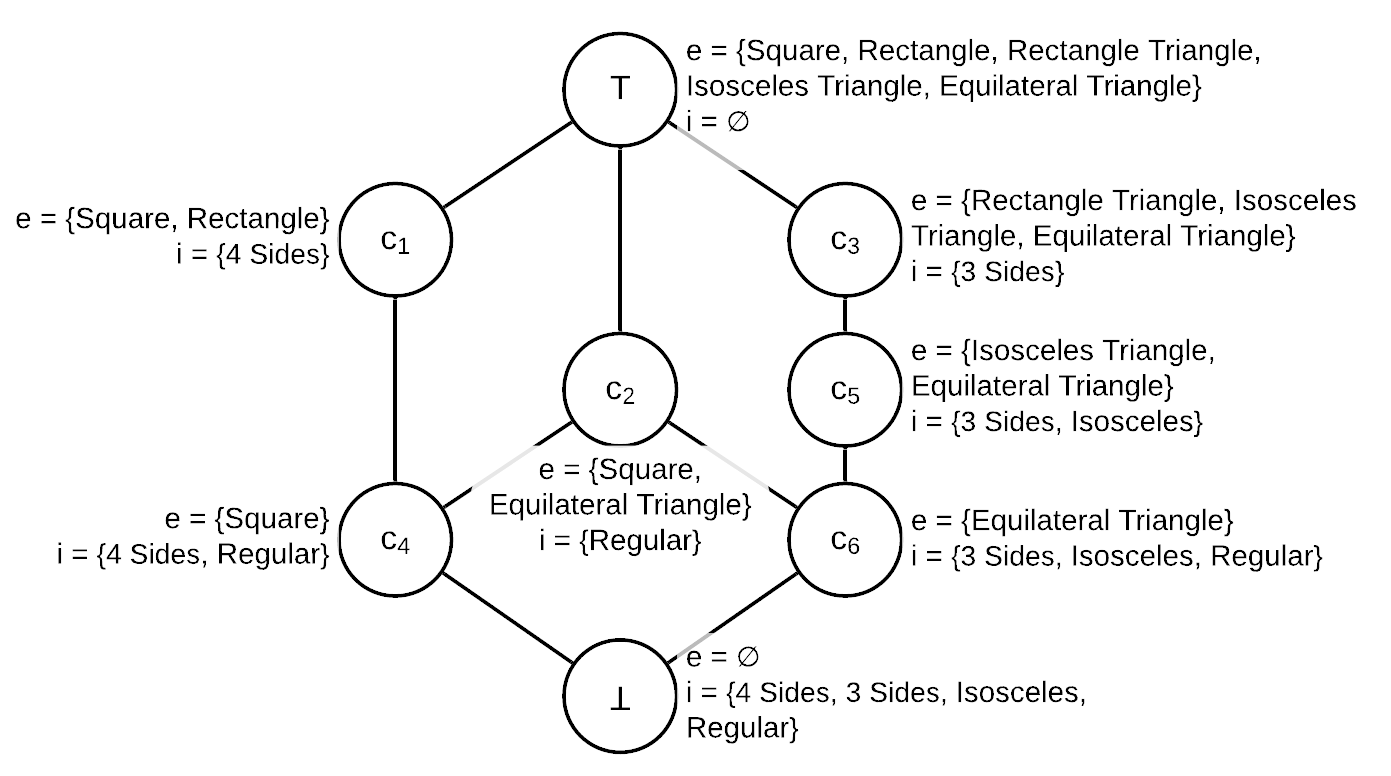
\includegraphics[keepaspectratio, width=\textwidth]{Figures/Ch0/example_full.png}}
    \caption{Lattice of the example context from \cref{fig:context}.}
    \label{fig:hasse}
\end{figure}

% \begin{figure}
%     \centering
%     \subcaptionbox{Context\label{fig:context}}{\scalebox{.8}{
%     %\subcaptionbox{Context\label{fig:context}}{\scalebox{1}{
%         $\begin{array}{rcccc}
%             &\rotatebox{90}{4 sides} & \rotatebox{90}{3 sides} & \rotatebox{90}{Regular} & \rotatebox{90}{Isosceles} \\
%             \text{Square} & \times & & \times & \\
%             \text{Rectangle} & \times & & & \\
%             \text{Rectangle Triangle} & & \times & & \\
%             \text{Isosceles Triangle} & & \times &  & \times\\
%             \text{Equilateral Triangle} & & \times & \times & \times\\%[4em]
%         \end{array}$}}
%     \subcaptionbox{Lattice\label{fig:hasse}}{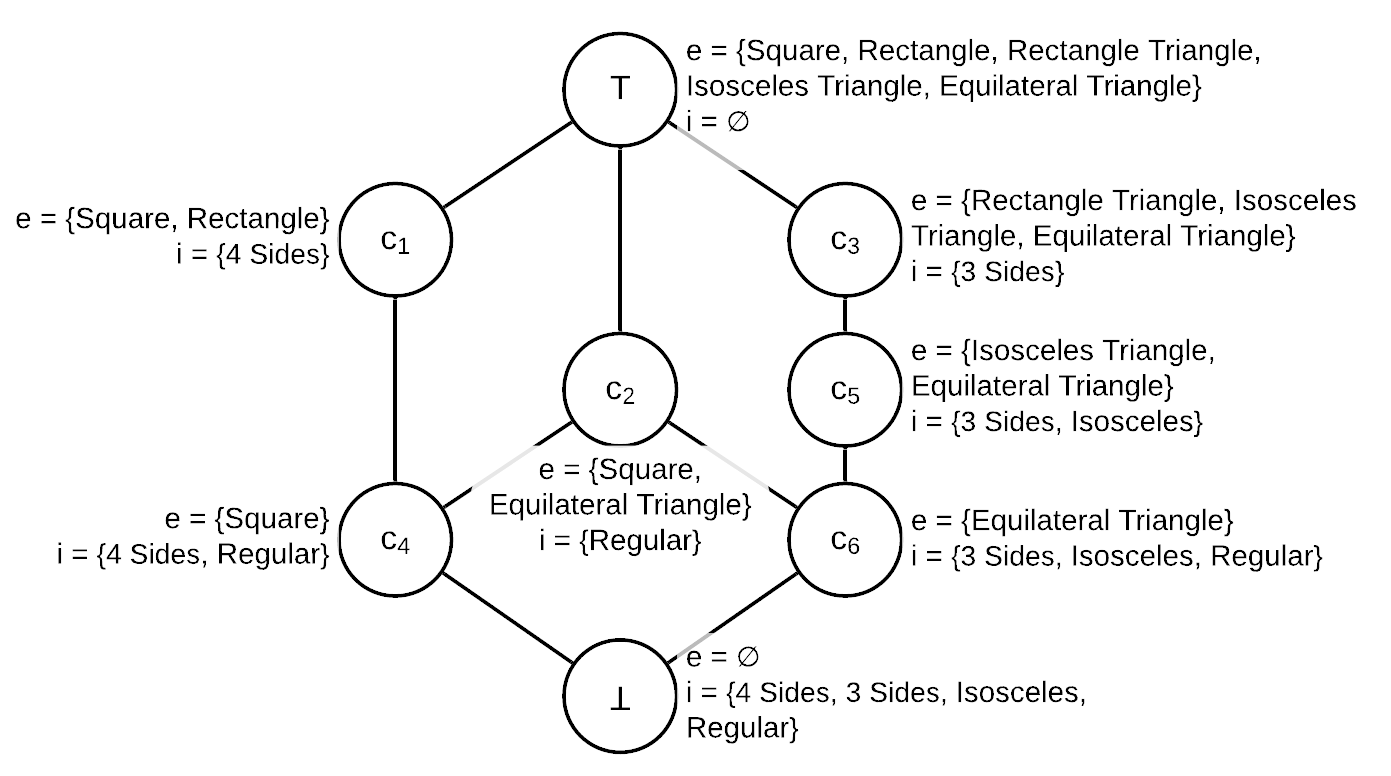
\includegraphics[keepaspectratio, width=.61\textwidth]{Figures/Ch0/example_full.png}}
%     %\subcaptionbox{Lattice\label{fig:hasse}}{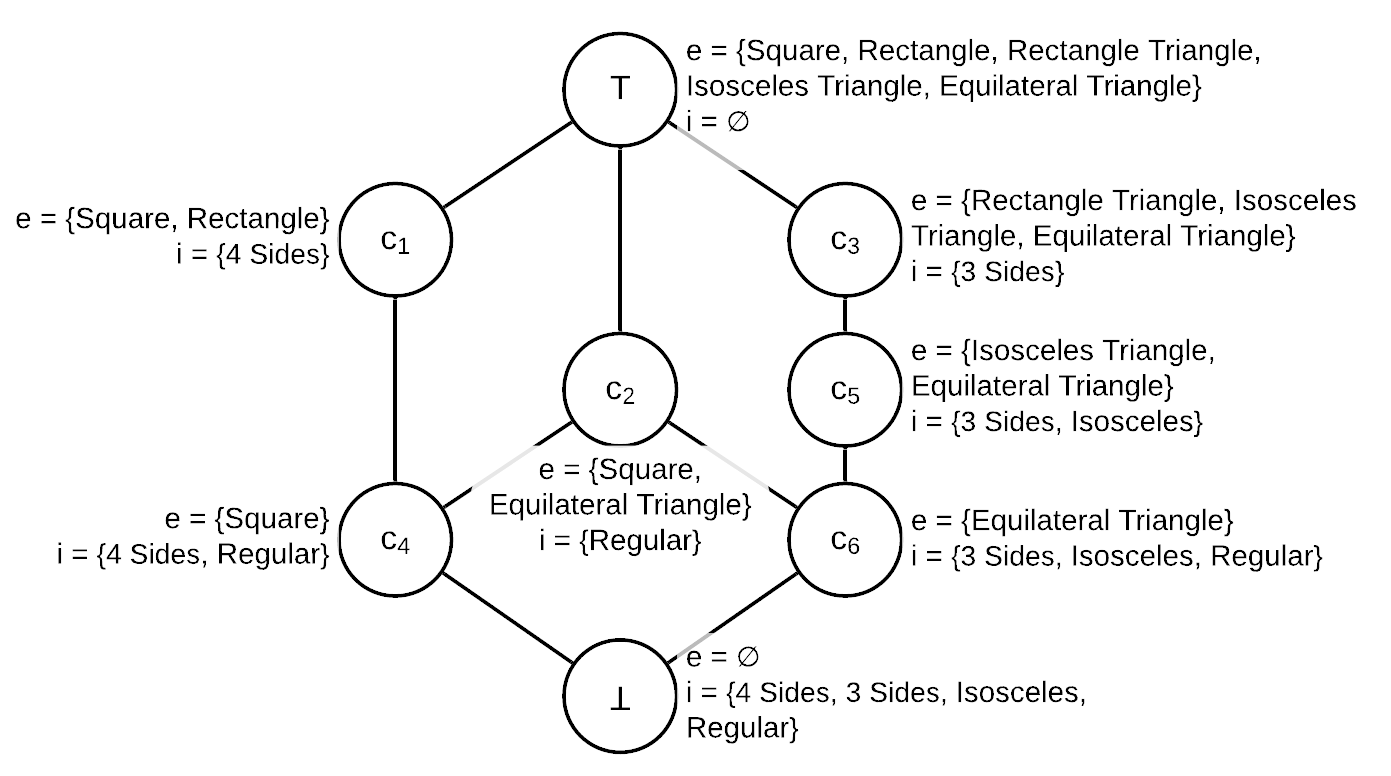
\includegraphics[keepaspectratio, width=.9\textwidth]{Figures/Ch0/example_full.png}}
%     \caption{Example of a formal context and the corresponding formal concept lattice.}
%     \label{fig:lattice-ex}
% \end{figure}

\subsection{Formal Concept Lattices Generation Algorithms\label{sec:lattice-algo}}
A naive way to generate concept lattices is to follow the definition of formal concepts.
The first step is to compute either the intents or the extents, and use it to build the set of formal concepts.
To achieve this, we can construct the set of extents as $E = \{Y'' \textrm{ for all } Y\in2^O\}$ and the set of concepts $\{\langle e', e\rangle \textrm{ for all } e \in E\}$.
The set of intents would be $I = \{X'' \textrm{ for all } X\in2^A\}$ and the set of concepts $\{\langle i, i'\rangle \textrm{ for all } i \in I\}$.
The number of possible extents and intents are respectively $|2^O| = 2^{|O|}$ and $|2^A| = 2^{|A|}$. The size of the set of concepts is thus, in the worst case, $2^{min(|O|,|A|)}$.
Therefore, assuming the time complexity of $\cdot'$ and $\cdot''$ is in $O(1)$, computing $E$ first is in $O(2^{|O|})$ and computing $I$ first is in $O(2^{|A|})$. In either case, there can not be a polynomial algorithm to build the set of concepts, because the size of the output (the set of formal concepts) is exponential to the size of the input (the FC).
%
The second step of our naive algorithm is to compute the order by comparing each pair of extents with $\subseteq$.

% Pour le calcul de la complexité pour l'énumération des concepts, tu annonces 2^|O| (ou 2^|A|). C'est vrai, mais ça mériterait peut être quelques mots de plus. Ici, on est dans un cas ou la taille de la sortie (l'ensemble des concepts) est exponentielle par rapport à l'entrée du problème (la taille du contexte).
% Dans ce cas, il ne peut pas y avoir d'algorithme polynomial pour résoudre le problème de l'énumération des objets (comme tu le mentionnes, même si on considère O(1) pour générer un concept, il faut passer tous les concepts, et il peut y en avoir un nombre exponentiel (au pire 2^min(|O|,|A|).

% Généralement, dans ce cas la (énumération d'une famille d'éléments en nombre exponentiel par rapport à la taille de l'entrée), on ne va pas s'intéresser à la complexité totale, mais à la complexité de génération par élément.
% Pour l'énumération d'ensembles fermés (resp. de concepts), la complexité par élément est entre O(n^2) et O(n^3) (ça dépend des algorithmes, et du fait d'avoir le droit ou pas d'utiliser un espace exponentiel).
% C'est intéressant parce que ça veut dire que, pour n'importe quel contexte pour lequel le nombre de concepts est polynomial en la taille du contexte, un algorithme d'énumération des concepts mettra un temps polynomial (en la taille de l'entrée).

% Par suite, je me demandais si, dans le cas de l'utilisation de méthodes de deep learning pour l'énumération des concepts, on retrouvait ce comportement... J'aurai tendance à dire non, puisque c'est le même réseau qui va être utilisé, mais je me demandais ce qu'on obtiendrait si on faisait des graphiques ou un axe comporte le ratio(nombre de concepts / Taille du contexte), la ou pour l'instant on a des graphiques avec le nombre de concepts seuls (dans l'article pour FCA4AI).

% Par exemple, il y a une sous-estimation du nombre de concepts dès qu'on dépasse 300 (graphique (a) page 10 de l'article pour FCA4AI))... mais est-ce que cette sous-estimation vient du nombre de concepts seulement, ou bien de la différence entre la taille du contexte et le nombre de contexte (autrement dit, prédit-on mieux 350 concepts sur des "gros" contextes que sur des petits ?)

There exist a wide variety of algorithms to generate concept lattices or at least the set of concepts.
For an overview of those algorithms see, \eg, \cite{comparing-fca-algorithms:2010:kuznetov}.
\section{Basic Background in Deep Learning\label{sec:background_nn}}
In this section, we recall some basic background in \textit{deep learning}. For further detail on NN architectures see, \eg, \cite{tuto-lstm:2019:staudemeyer}.

\subsection{Neural Networks\label{sec:nn}}
\textit{Neural networks} (NNs) are a class of statistical connectionist models trained using the \textit{backpropagation} algorithm.
The training is done by processing inputs with the model and evaluating the quality of the output using a \textit{loss function}.
By minimizing this loss with an optimization algorithm, the model learns to approximate the expected output.
In this subsection, we detail several kinds of model designs (or \textit{architectures}) frequently used in deep learning.

%For detailed information on the neural architectures mentioned in this paragraph, we recommend~\cite{tuto-lstm:2019:staudemeyer}.
A multi-layer perceptron (MLP) is the simplest architecture of NN.
It is composed of multiple layers, called \textit{feed-forward layers}.
Each output of a feed-forward layer is a linear composition of all the layer's inputs.
Between layers, the values are transformed by an \textit{activation function} to increase the expressive capacity of the model.
The \textit{rectified linear unit} (ReLU) and \textit{sigmoid} are among the most common activation functions.
\cref{fig:basic-nn-architectures} contains a simple diagram of the MLP.

\begin{figure}
    \centering
    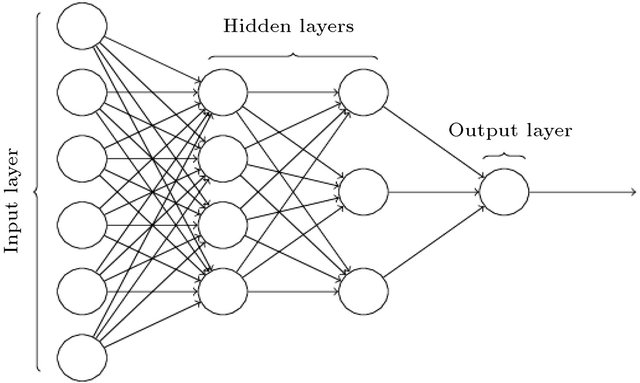
\includegraphics[keepaspectratio, width=.9\textwidth, height=5cm]{Figures/Ch0/mlp}
    \caption{Multi-layer perceptron architecture. From \footnotesize{\url{https://www.researchgate.net/profile/Ayhan_Erdem2/publication/319309006}}.}
    \label{fig:basic-nn-architectures}
\end{figure}

\subsection{Deep Learning Algorithms}
To train NNs we use specific algorithms called \textit{optimizers} to update the \textit{parameters} of the NN model based on the value of a loss function.
The parameters are the numerical values involved in the NN computations.% In the case of an MLP, the parameters are the coefficients of the linear composition functions of all the neurons of all the layers.

Training is performed by iteratively updating the \textit{parameters} of the NN, by presenting it with \textit{batches} (groups) of input samples and applying the optimizer based on the loss.
An \textit{epoch} is when all the data available is processed once.
The process is usually repeated for multiple epochs until the model \textit{converges}, in other words, until the performance of the model stops improving.

There exist a variety of optimizers, but the most recommended one~\cite{optim:2016:ruder} currently is Adam~\cite{adam:2015:kingma}.
For an overview of existing optimizers see, \eg, \cite{optim:2016:ruder}.
In our experiments, we use Adam.
This particular algorithm has low computational and memory usage compared to other algorithms and is well suited for complex optimization problems.

\subsection{Usual Loss Functions}
The loss function to use depends on the kind of problems handled.
%
When predicting specific values within a set of known values, it is standard to make the NN output probabilities of being in each of the possible values.
Typical examples are classification problems and language modeling, where the model has to predict the most likely character or word among known ones.
For those problems, we usually use the \textit{cross-entropy} loss to make the predicted probabilities closer to the actual ones.
In the binary case (only 2 possible values), we use the \textit{binary cross-entropy} (BCE) which only requires the probabilities of one of the two classes. \cref{equ:ce} is the equation of the cross-entropy with $X$ the set of all possible values, $p$ the target distribution, $q$ the predicted distribution, and $p(x)$ (or $q(x)$) the probability to have the value $x$ according to $p$ (respectively $q$). \cref{equ:bce} is the equation of the BCE with two values $0$ and $1$, but computed only using $1$.
%
Another common kind of problem is predicting real-valued data or integers, \eg, image generation.
In those cases, we typically use \textit{mean squared error} (MSE) to reduce the squared distance between the predicted value and the expected one.
\cref{equ:mse} is the equation of the MSE with $p$ and $q$ the target and the prediction.
%
Other loss functions are widespread, \eg, the cosine similarity, but we mainly use cross-entropy, BCE, MSE, and loss functions derived from those three.

\begin{align}
    H(p, q) =& - \sum_{x\in X} p(x) log(q(x)) \label{equ:ce}\\
    BCE(p, q) =& - p(1) \times log(q(1)) - (1-p(1)) \times log(1-q(1))\label{equ:bce}\\
    MSE(p, q) =& \sum_{i = 1}^{|p|}(p_i - q_i)^2\label{equ:mse}
\end{align}

\subsection{Binary Encoding and Softmax}
In classification problems the possible values are usually indexed, and a specific label is represented by a binary vector.
We speak of the \textit{binary encoding} of a set of values and \textit{one-hot encoding} of a value. Those encodings are computed with regards to the indexed set of all possible values.
In our setup, the binary encoding of a set of attributes $X \subseteq A$ is the vector of size $|A|$, such that the position $k$ of the vector contains $1$ if $a_k\in X$ and $0$ otherwise. The one-hot encoding of an attribute $a_k$ is the binary encoding of $\{a_k\}$, in other words the vector of size $|O|$ full of $0$ except at position $k$ which is $1$.

When performing a single-label classification, we usually generates the probablility for each value to be the correct one.
To obtain this set of probabilities we usually use the \textit{softmax} function, which transforms any finite set of numbers into a probability distribution.
In other words, it transforms the values into probabilities (between 0 and 1) in such a way that the sum of all values is equal to 1 and that the proportions between the values are preserved.

%In this section, we use the notions of \textit{binary} encoding of a set and \textit{one-hot} encoding of an element. Those encoding are computed with regards to the indexed set of all possible values.

%In this section we introduce the \textit{softmax} function, which transforms any finite set of numbers into a probability distribution.
%In other words, it transforms the values into probabilities (between 0 and 1) in such a way that the sum of all values is equal to 1 and that the proportions between the values are preserved.

\subsection{Major Neural Networks Architectures}
A \textit{convolutional neural network} (CNN) is a NN that apply \textit{convolutions} on an input. For an overview of CNN see, \eg, \cite{cnn-overview:2018:yamashita}.
Following the principle of \textit{convolutions}, for a given input element, a CNN produces an output based on a learned \textit{kernel} and the neighborhood of the input. It is possible to compute the size of the output and the size of the neighborhood taken into account by the CNN.
A CNN can handle inputs of varying sizes, and the output size is proportional to the ones of the input.
Additionally, CNNs maintain the relations between neighboring elements and is invariant to translation.
In other words, a CNN will produce the same output for a given neighborhood at different locations in the input.
They are widely used in image processing due to this property allowing it to learn filters to detect features independently of the position in the input.
A basic CNN is shown in \cref{fig:nn-architectures-cnn}.

\begin{figure}
    \centering
    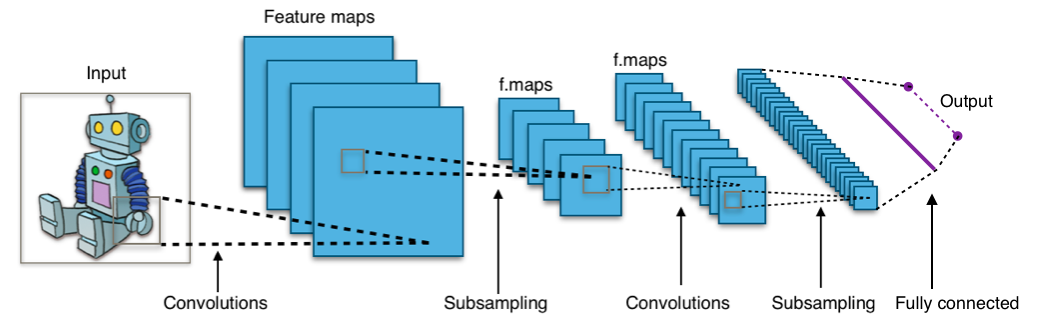
\includegraphics[keepaspectratio, width=.9\textwidth, height=5cm]{Figures/Ch0/cnn.png}
    \caption{Example of CNN architecture. From Wikipedia.}
    \label{fig:nn-architectures-cnn}
\end{figure}

The famous \textit{long short-term memory recurrent NN} (LSTM)~\cite{blstm:2005:graves} and \textit{gated recurrent unit NN} (GRU)~\cite{gru:2014:cho} are architectures of a family called \textit{recurrent NNs} (RNNs).
This family of models handles sequences of inputs of variable length, and are designed to learn dependencies within the input sequence.
By transmitting and updating a vector called \textit{hidden state} from one step of the sequence to the following one, each output depends on the current input as well as the previous ones.
A variant of the LSTM, called \textit{bi-directional LSTM} (BLSTM)~\cite{blstm:2005:graves}, uses a second LSTM to process the input sequence in the reverse direction. It can thus handle both forward and backward dependencies in the sequence.
A major flaw of all RNNs is their inability to model long-range dependencies, with various variants like LSTM and GRU trying to solve this \textit{memory} issue to some extent.
A block diagram representing how RNN handle sequences is shown in \cref{fig:nn-architectures-rnn-unfolded}, and the inner workings of a a GRU and an LSTM are shown respectively in \cref{fig:nn-architectures-gru}, and \cref{fig:nn-architectures-lstm}.

\begin{figure}
    \centering
    \subcaptionbox{RNN\label{fig:nn-architectures-rnn-unfolded}}{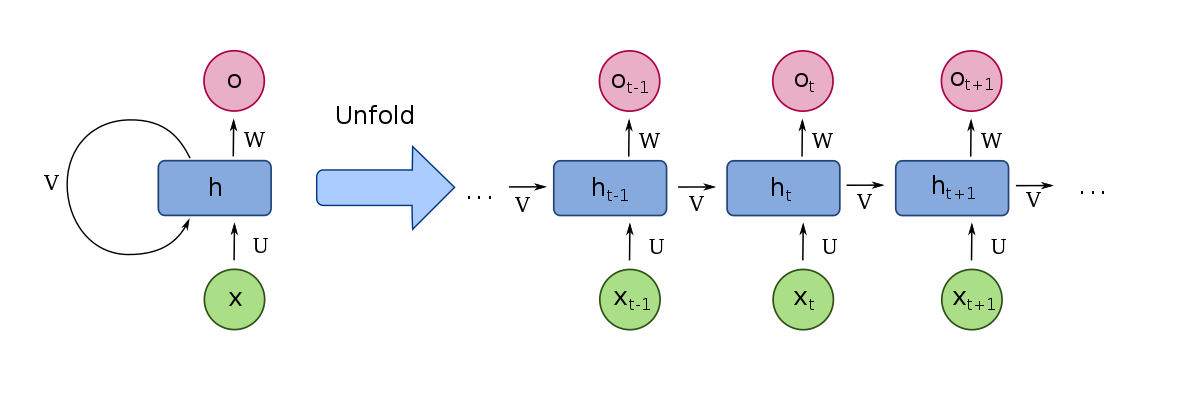
\includegraphics[keepaspectratio, width=.9\textwidth, height=4cm]{Figures/Ch0/rnn.png}}
    \subcaptionbox{GRU cell\label{fig:nn-architectures-gru}}{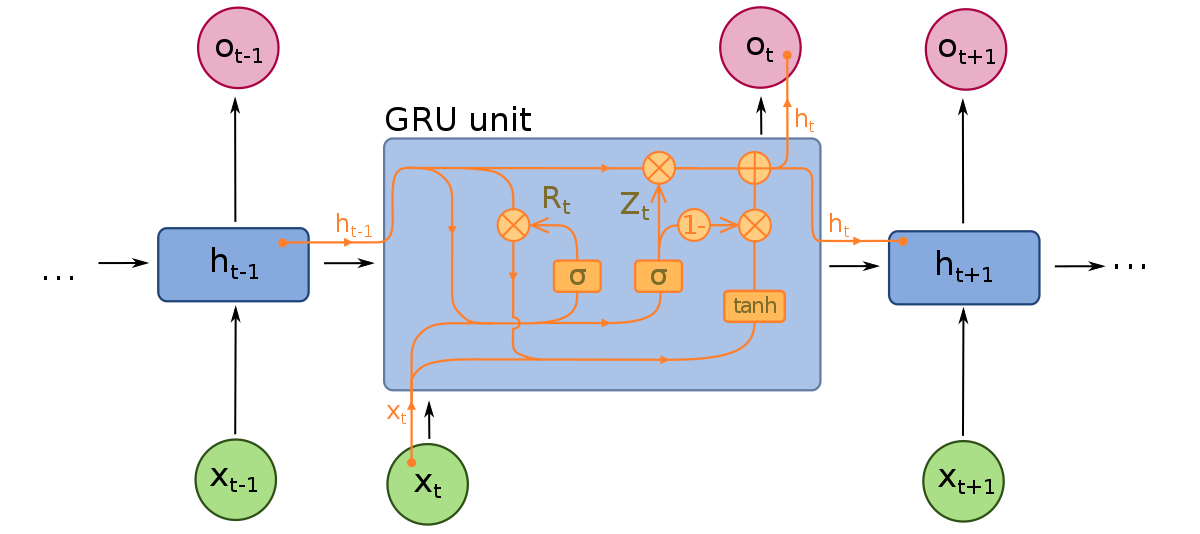
\includegraphics[keepaspectratio, width=.48\textwidth, height=5cm]{Figures/Ch0/gru_cell.png}}
    \subcaptionbox{LSTM cell\label{fig:nn-architectures-lstm}}{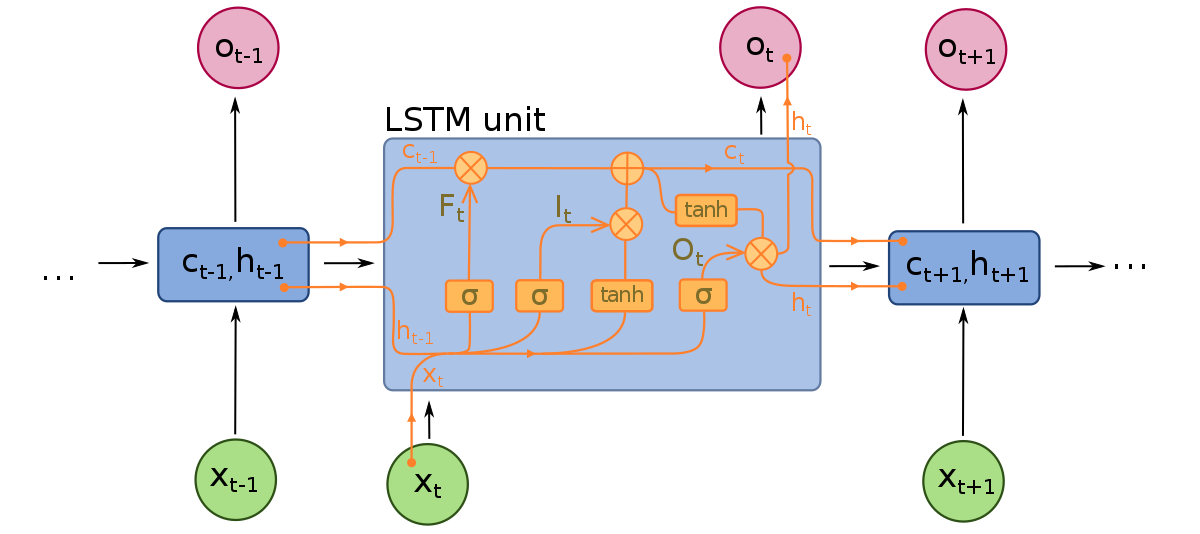
\includegraphics[keepaspectratio, width=.48\textwidth, height=5cm]{Figures/Ch0/lstm_cell.png}}
    \label{fig:nn-architectures-rnns}
    \caption{Structure of the major RNN architectures, the input at step $t$ is $x_t$, the hidden state $h_t$, and the output $o_t$. From Wikipedia.}
\end{figure}

\textit{Attention} mechanisms~\cite{attention:2015:bahdanau}, which have been developed to handle this issue, consider a full sequence and attribute \textit{attention weights} to each element. The attention weights are usually computed with a \textit{dot product} between a \textit{query} and the elements in the sequence, though there are numerous variants of attention. The attention weights are usually used to weight the sequence directly or to compute a weighted average of the sequence.
The summaries produced by the attention mechanisms are called \textit{context}.
Attention is cheap to compute (usually), and the analysis of the attention weights allows to determine the implication of each element in the final result.
Due to this property, attention can be used to make an RNN's result interpretable.
Attention is powerful enough to be used alone, like the \textit{transformer network}~\cite{transformer:2017:vaswani} and more recently the \textit{reformer network}~\cite{reformer:2020:kitaev}.
An example of attention for neural machine translation is shown in \cref{fig:nn-architectures-attention}.

\begin{figure}
    \centering
    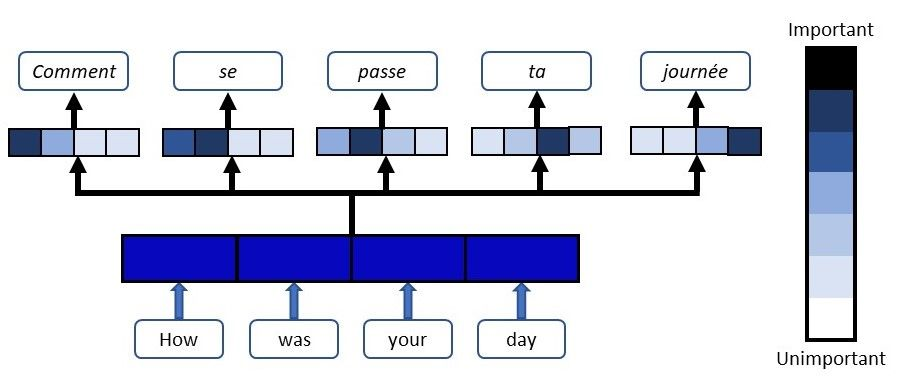
\includegraphics[keepaspectratio, width=.9\textwidth, height=5cm]{Figures/Ch0/attention.jpg}
    \caption{Example of attention mechanism for translation from English to French. From \footnotesize{\url{https://blog.floydhub.com/attention-mechanism/}}}
    \label{fig:nn-architectures-attention}
\end{figure}

We call \textit{unordered composition functions} operations that do not take into account the order of the input elements and can accommodate any number of input elements. Typical examples for vectors are the element-wise min, max, and average (also respectively called min-, max-, and average-pooling).
Unordered composition-based models combining an unordered composition of the inputs with an MLP are called \textit{deep averaging networks} (DANs).
They have proven their effectiveness in a variety of tasks, for instance, sentence embedding~\cite{dan:2015:iyyer}, sentiment classification~\cite{adan:2016:chen}, and feature classification~\cite{cdan:2017:gardner}.
On the one hand, this family of architectures allows for varying sizes of input to be processed at a relatively low computational cost, by opposition to recurrent models like LSTM.
On the other hand, the information related to the order of the input elements is lost.
The DAN for sentence embedding from~\cite{dan:2015:iyyer} is shown in \cref{fig:nn-architectures-dan}.

\begin{figure}
    \centering
    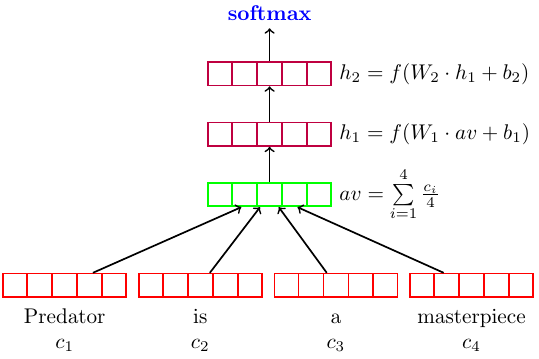
\includegraphics[keepaspectratio, width=.9\textwidth, height=5cm]{Figures/Ch0/dan.png}
    \caption{Example of DAN, Figure 1 from~\cite{dan:2015:iyyer}.}
    \label{fig:nn-architectures-dan}
\end{figure}

To summarize, CNNs, RNNs, attention mechanisms, and DANs are various architectures able to handle inputs of varying sizes, each with their advantages and drawbacks.

\subsection{Auto-Encoders and Embeddings\label{sec:vae}}
\textit{Auto-encoders} are a class of deep learning models composed of:
\textit{(i)} an encoder, taking some $x$ as an input and producing a latent representation $z$;
\textit{(ii)} a decoder, taking $z$ as an input and reconstructing $\hat{x}$ a prediction of $x$.
%The model learns to reresent $x$ into $z$ with a the training objective
By training the model to match $x$ and $\hat{x}$, the model learns to compress $x$ into $z$. We call the training objective matching $x$ and $\hat{x}$ the \textit{reconstruction loss}.
Auto-encoders are one of the methods to generate representations of data as vectors. In that case, $z$ is called the \textit{embedding} of $x$, and the real-valued space in which $z$ is defined is called the \textit{embedding space}.

%\subsubsection{Variational Auto-Encoders}
Unlike traditional auto-encoders, \textit{variational auto-encoders} (VAEs)~\cite{vae:2013:kingma} encode a distribution for each value of $z$ instead of the value itself.
In practice, for each element of $z$, the encoder produces two values: a mean $\mu$ and standard deviation $\sigma$.
When training the model, $z$ is sampled from the normal distribution defined by $\mu$ and $\sigma$.
Finally, the distribution defined by $\mu$ and $\sigma$ is normalized by using an additional loss term called \textit{Kullback–Leibler divergence} (KL divergence).
To make this process differentiable and be able to train the model, a method called \textit{reparametrization}~\cite{vae:2013:kingma} is used.

VAEs are known to provide better generalization capabilities and are easier to use to decode arbitrary embeddings, compared to classic auto-encoders.
This property is useful for generation, as we can train a model generating embeddings then decode them with a pre-trained VAE.
A typical example of VAE, is one trained on basic geometric shapes (circles, triangles, rectangles, \etc), allows us to decode arbitrary embeddings:
the average of the embedding of a triangle and a rectangle would give us a trapezoid (a coherent mix of a triangle and a rectangle) even if none were seen during training.
Thus, VAEs have been used in a wide variety of applications to improve the quality of embedding spaces: image~\cite{vae:2013:kingma}, speech~\cite{deep-metric-multispeaker:2020:kulkarni}, and graph generation~\cite{graph-vae:2016:kipf} for example.
%However, using a VAE instead of a classical auto-encoder can decrease the performance for some tasks.\todo{add citation}
%To use a VAE as an encoder once it is trained, we do not sample $z$ from the distribution and use $\mu$ .
% \begin{figure}
%     \centering
%     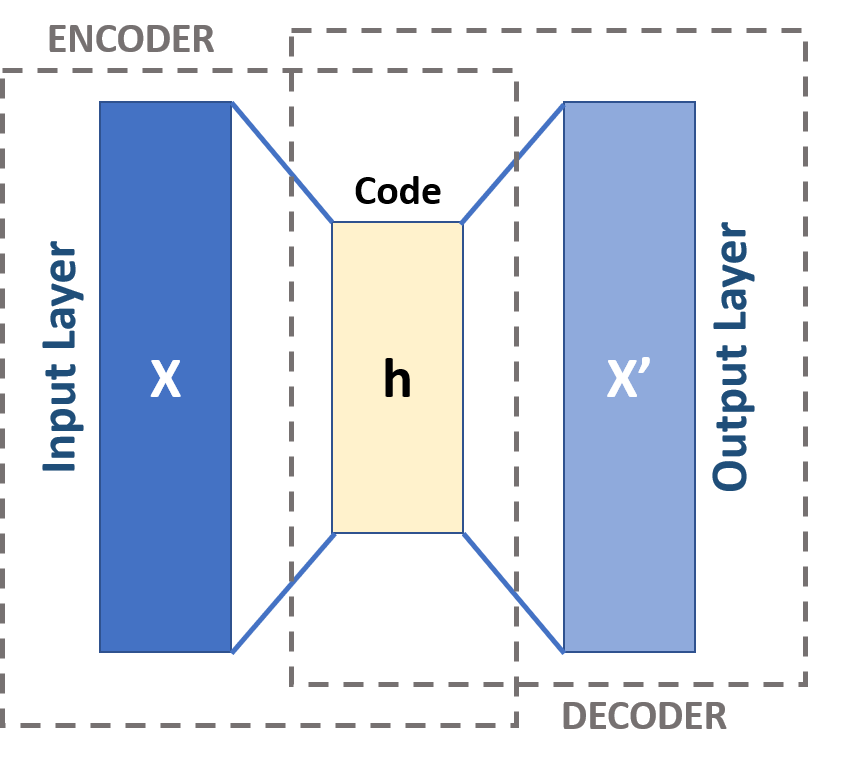
\includegraphics[keepaspectratio, width=.9\textwidth, height=5cm]{autoencoder_wiki}
%     \caption{Diagram of a basic auto-encoder. From \url{https://en.wikipedia.org/wiki/Autoencoder}.}
%     \label{fig:my_label}
% \end{figure}


A constrained VAE is a kind of VAE that feeds a \textit{constraint} vector (or \textit{condition}) to the decoder in addition to the embedding.
Because the condition already contains part of the information, the model will learn to encode the rest in the embedding.
This architecture allows to voluntarily exclude part of the information form the embedding or to constrain the decoding process.
An example of constrained VAE is~\cite{deep-metric-multispeaker:2020:kulkarni}, which uses the condition to specify the speaker in emotional speech.
The embedding contains ``anonymized'' speech information, and it becomes possible to transfer emotional speech from one speaker to another by changing the condition.

\subsection{Metric Learning}
\textit{Metric learning}~\cite{vae-metric-learning:2018:xudong} is a process used to train embedding models, by making their embedding space have properties of a metric.
To achieve this, a loss is used to reduce the distance between the embeddings of equal elements and increase the distance between embeddings of different elements.
Multiple losses can achieve this, such as \textit{pairwise loss} and \textit{triplet loss}. 
Those losses consider the embeddings of three elements: an input $x$, some $x'$ judged equal to $x$, and some $y$ different from $x$.
They are used to minimize the distance between equal elements and maximize the distance between different elements.
In some approaches~\cite{deep-metric-multispeaker:2020:kulkarni}, a predictor (typically an MLP) is used to predict a distance between the embeddings, instead of applying a standard distance directly on the embeddings.

It is possible to learn metrics on different aspects of the elements, by splitting the embedding into different segments and learn a different metric on each segment~\cite{deep-metric-multispeaker:2020:kulkarni}.

Metric learning is usually used to approximate actual metrics.
However, its process can be applied to learn other kinds of measures not fitting the definition of a metric.
The current paper falls in this case.
\section{Problem Statement\label{sec:problem}}
Our main objective for this project is to provide a grounded proof of concept, demonstrating the feasibility of concept lattice generation using NNs.
We focus on providing a fully working and general framework, able to handle unseen FCs with no technical constraint on the size.
The generation performance and the explainability are also taken into account, but they are secondary. Indeed, extensive training of the model can easily boost the performance once the framework is designed. Additionally, we orient our design choices to facilitate the integration of explainable methods in future work.
Finally, we do not consider the computational optimization of the methods as a major concern.

In the previous section, we saw that a formal concept lattice is defined by a set of concepts and a partial order relation between the concepts.
Given the relations between the order relation $\leq$, $<$, and $\prec$, a single one of them is enough to describe the partial order between the concepts.
Also, the set of concepts can be completely described using either the set of intents or the set of extents.
%
From those two aspects, we can apply the principle of ``divide and conquer'' to split the difficult task of lattice generation into simpler tasks:
on the one hand, generating the order between the concepts, and on the other hand, defining the concepts themselves.
Additionally, the order relation can be described by graphs (\eg, the graphs of $<$ and $\prec$), with the concepts being the nodes of the graph, so \soa{}, methods in graph generation can be used.

Two approaches can be devised to solve the tasks of generating the concepts and the order between them: (\textit{i}) generating the order between the concepts first and then defining the concepts, and (\textit{ii}) generating the concepts, then computing the order relation between them. Each of these approaches focuses on a different aspect of the formal concept lattice.
We explore the first approach in \cref{ch:graph} by adapting \soa{} methods to generate the graphs of lattices.
In \cref{ch:intents}, we focus on generating the intents using the information from the FC, thank to the BoA embedding model for FCs described in \cref{ch:boa}.

Our choice of working with the intents to define the concepts comes from the assumption that $|A| \leq |O|$ in most datasets, so focusing on intents should be less costly than with the extents as fewer elements are involved.
In cases where this assumption is not verified ($|A| > |O|$), we can exchange the objects and the attributes.
Indeed, if we exchange them the resulting lattice is the same, except $\leq$ and $\prec$ which respectively become $\geq$ and $\succ$, and the intents and extents which are swapped with one another.
In practice, this exchange of $A$ and $O$ corresponds to using the transposed $C$ instead of $C$ itself.
It is easy to swap back the intents and extents in the output and to reverse the order and cover relations to get the expected lattice.
In simple words, whether we design our method by focusing on intents or extents, we can adapt it to the other case with simple transformations.

% For both approaches, our main objective is to provide a grounded proof of concept, demonstrating the feasibility of concept lattice generation using NNs.
% Our main goal is to provide a fully working and general framework, able to handle unseen FCs with no technical constraint on the size.
% The generation performance and the explainability are secondary goals, and we do not consider the computational optimisation of the methods as a major concern.
%To achieve our goals, we first study the existing methods and decide on the representation to use for the FCs and the lattices.
%We then design the NN architecture to use and perfrorm qualitative or quantitative experiments on a dataset of FCs and the corresponding lattices.
%We iterate between the designa and the experimental steps, untill
 

\chapter{Initial Approach: Graph Generation\label{ch:graph}}
In this chapter we explore the reconstruction of the lattice as a relation between formal concepts.
As a relation corresponds to a graph, we can use the \soa{} graph-generation methods described in \cref{sec:graph-soa} to generate the lattice.

Our goal which is to learning a single model to generate all the lattices leads us to focus on models able to generate families of graphs. In particular, we selected GraphRNN~\cite{graphrnn:2018:jiaxuan}, for the reasons explained in \cref{sec:graphrnn-choice}, and adapted it into a constrained VAE presented in \cref{sec:graph-model}. We also adapted their graph encoding method to represent lattices as we describe in \cref{sec:data-format}.

We performed preliminary experiments with this method as described in \cref{sec:graph-expe}.
However, the challenge of how to use the FC as a condition for the VAE, together with the relatively poor generation performance, led us to put aside the graph generation approach and focus on generating the concepts first, as described in \cref{ch:intents}.
The BoA embedding framework, described in \cref{ch:boa}, is the result of our tentative to make the FC usable as a condition for the VAE.
As we did not finalize the approach, the corresponding code is not present in our GitLab repository.%\todo{jump to ch4}


\section{State of the Art of Graph Modeling\label{sec:graph-soa}}

%\todo[inline]{This whole section uses ``generation'', ``modeling'', ``handle'' etc. It is necessary to check the use of the terms and find better suited terms if necessary. > generative model}


In recent years, there has been an explosion of approaches to model graphs with NNs. Typical applications are knowledge graph processing and community graph detection.
There exist a variety of approaches to graph modeling in the literature. In this section, we describe the main approaches of graph representation and generation, and their principal characteristics.
For further details see, \eg, \cite{graph-nets:2019:many-authors} or the repository \url{https://github.com/dsgiitr/graph_nets}.

%The various approaches for graph modeling using NNs vary along 2 major aspects. the data representation method and algorithm on one side, and what the model is capable of modeling on the other side.
The various approaches for graph modeling using NNs vary along 2 major aspects: the data representation method and the kind of objects that the framework is capable of modeling, \eg, individual nodes or whole graphs.
%
Firstly, the representation and processing of the graph differ in how the two major aspects of the graph are represented.
On the one hand, the structure of the graph is the adjacency between the nodes. It can be represented as an adjacency list, an adjacency matrix, a graph spectrum (see \cref{sec:soa-graph}), or implicitly by considering the neighborhood of a node.
On the other hand, nodes can be represented either implicitly by only considering the structure of the graph, by an arbitrary identifier like a random value, or by a set of features or labels.
As a reminder, \textit{features} of nodes in a graph are a set of properties contained in nodes, \eg, the name, age, and email address in a social network.
\textit{Labels} are textual or numerical denominations of the nodes and edges, and can be seen as a specific kind of features.
%
%A graph NN can represent either nodes within graphs or whole graphs of a specific family.
%A \textit{family} of graphs is a set of graphs sharing some specific structural properties, \eg, community graphs and ontologies.
%Representing a node within a particular graph allows to manipulate node representation, \eg{} generating entity embeddings for knowledge graphs, where entities are nodes.
%Graph NNs representing whole graphs are used to represent a specific class of graphs. In other words, they are trained to handle graphs sharing some specific structural properties, \eg{} community graphs.
Secondly, graph NN can represent either nodes or whole graphs.
We detail those two kinds of graph NNs respectively in \cref{sec:soa-node} and \cref{sec:soa-graph}, along with major graph NNs approaches.
We explain why we chose to focus on GraphRNN in \cref{sec:graphrnn-choice}.

%%%%%%%%%%%%%%%%%%%%%%%%%%%%%%%%%%%%
\subsection{Node-Centered Approaches\label{sec:soa-node}}
The first group of graph NNs focuses on representing nodes.% within a single graph.
This kind of NN can be trained on a specific graph to provide representations for this graph's nodes~\cite{word2vec:2013:mikolov,deepwalk:2014:perozzi}.
It is used to generate local representations in particular for large and complex graphs, \eg{}, generating entity embeddings for knowledge graphs or node embeddings for community graphs.
Graphs NNs representing nodes can also be used to represent whole graphs, by combining the representation of the nodes.
However, it is also possible to learn a more general model to represent nodes by training on multiple graphs~\cite{gcn:2016:kipf}.

A first method, proposed in DeepWalk~\cite{deepwalk:2014:perozzi}, is to mimic natural language processing (NLP) methods for learning sentences.
The neighborhood of a node is \textit{linearized}, by taking a sequence of nodes obtained by randomly walking through the graph.
The sequences of nodes are then processed as if they were sentences, with SkipGram~\cite{word2vec:2013:mikolov} in the case of DeepWalk.

A second approach is \textit{message passing}, in which a node representation is built iteratively.
The nodes' initial representation can be the features of the nodes (represented as vectors), or randomly generated values if there are no given features for the nodes.
GraphSAGE~\cite{graph-sage:2017:hamilton} and Graphite~\cite{graphite:2018:grover} are examples of message passing neural algorithms, with~\cite{graphite:2018:grover} including a variational version of the Graphite.

A third framework is \textit{graph convolution}, an adaptation of CNNs from grid-like structures like images to the more irregular structure of graphs.
In practice, the kernel is applied to the neighborhood of a node as defined in graphs, instead of the spatial neighborhood of a cell in a matrix.
Graph Convolutional Network (GCN)~\cite{gcn:2016:kipf} is the basic architecture implementing this approach, and Hypergraph Neural Network~\cite{hypergraph-nn:2018:feng} is an adaptation of GCNs to hypergraphs.
Graph Attention Network (GAT)~\cite{gat:2017:velickovic}, Masked GCN~\cite{masked-gcn:2019:yang}, SPAGAN~\cite{spagan:2019:yang}, Hierarchical GAN~\cite{hierarchical-gan:2019:kim} are improvements of GCNs with attention mechanisms and other similar techniques. Those improvements allow the NN to select neighboring nodes based on the current node and the content of the neighbors.

%spatial convolution (neighborhood): Graph Convolutional Network (GCN)~\cite{gcn:2016:kipf}, Hypergraph Neural Network~\cite{hypergraph-nn:2018:feng}
%attention (giving different weights to different neighbors, depending on some features of the nodes):
%Graph Attentional Network \todo[inline]{check name} (GAT)~\cite{gat:2017:velickovic}, Masked GCN~\cite{masked-gcn:2019:yang}, SPAGAN~\cite{spagan:2019:yang}, Hierarchical GAN~\cite{hierarchical-gan:2019:kim}.

%%%
\subsection{Whole Graph Approaches\label{sec:soa-graph}}
Graph NNs representing whole graphs are used to represent graphs from a specific \textit{family} (or class) of graphs. In other words, they are trained to handle graphs sharing some specific structural properties, \eg, community graphs.
This kind of graph NNs are used to perform tasks on a whole graph at once, \eg, classification of a graph and generating graphs of a specific family.

A first method is \textit{spectral convolution}, introduced in~\cite{spectral-nn:2014:bruna} and with a more recent implementation called ChebNet~\cite{chebnet:2019:tang}.
Spectral convolution is based on spectral graph theory, which represents a graph's adjacency using a spectrum.
The spectrum of a graph provides a complete view of the graph's adjacency.
A detailed introduction to spectral graph theory can be found, \eg, in~\cite{spectral-graph-lectures:1996:chung}.
Spectral convolution is an application of CNNs on this spectrum of the graph.

A second framework is \textit{hierarchical graph pooling}, presented in~\cite{hierarchical-graph-pooling:2018:ying}.
This method is an iterative simplification of the graph by grouping strongly related nodes using clustering and pooling methods.
Once a single group remains, the graph is fully simplified.

A third approach is to use a VAE directly on the adjacency matrix of a graph, as implemented in GraphVAE~\cite{graph-vae:2016:kipf} and Constrained GraphVAE~\cite{constrained-graph-vae:2018:ma}.
By flattening the adjacency matrix to a vector, it becomes possible to apply a VAE directly on the adjacency.
This method performs well at generating graphs of specific families, despite being less involved than the other methods presented in this section.
Indeed, it doesn't rely on specific properties of graphs to establish its architecture.

A fourth method is to use recurrent models on a linearization of the graph, as done in GraphRNN~\cite{graphrnn:2018:jiaxuan}.
In this approach, the graph is first transformed into a sequence of nodes, and the nodes are then processed iteratively.
GraphRNN processes each node of the sequence by computing its edges with the previous nodes in the sequence.
They rely on a breadth-first search to linearize the graph to make connected nodes close in the sequence.

\subsection{Advantages of GraphRNN for Lattice Generation\label{sec:graphrnn-choice}}
As a reminder, our goal is to learn a single neural model to generate lattices in general. We want the model to produce a whole lattice for each FC presented.
From those constraints, we focus on graph NNs able to handle whole graphs at once.
The architecture should also be able to generate graphs, and only GraphVAE, Constrained GraphVAE, and GraphRNN fit our criterion.

A drawback of GraphVAE and Constrained GraphVAE is that they are limited in the size of the graph they can handle.
Indeed, VAE has a fixed-sized input and output, so the two approaches are unable to handle graphs larger than the graphs they are trained on.
Conversely, the recurrent nature of GraphRNN makes it very flexible with regard to the size of the generated graphs.

A final argument in favor of GraphRNN is that it is easily extendable with node features.
In our case, node features are the intent and extent of the concepts, and they are very important for our goal because they define the concept.
In practice, when generating a new node, we would add a network to generate the intent or the extent to the link generation network of GraphRNN, as we explain in \cref{sec:graph-model-full}.

GraphRNN shows \soa{} performance when generating graphs of various families, and can handle any size of graphs.
However, it is not designed to generate specific graphs on request, as we would like to do to generate lattices based on the FCs.
Conversely, constrained VAEs (such as Constrained GraphVAE~\cite{constrained-graph-vae:2018:ma}) are generative models that can be constrained.
Using such a model would allow us to generate lattices under the constraint of the FCs.
To compensate for the limitations of GraphRNN with regards to our goal, we decided to adapt GraphRNN into such a constrained VAE.
As described in \cref{sec:graph-model}, we first adapt GraphRNN into an auto-encoder, which is later adapted into a VAE and then further modified as a constrained VAE.


\section{Transforming Lattices into Matrices\label{sec:data-format}}
When training a NN on non purely numerical data, lattices in our case, it is necessary to first represent the data in a numerical form.
The choice of the data, as well as the quality of the representation, noticeably affect the quality of the resulting model.
Typically, a bad representation makes learning hard if not impossible, while a well-thought representation of the data is already half the job done.
Also, the model will perform better and be better at generalizing when trained on more and more varied data.
%The choice of the data representation and of the model architecture are dependent on each other. 

We decide to learn on randomly generated FCs and the corresponding lattices.
The main reason is that gathering and preparing large amounts of usable real-world FC is costly, while generating random data is cheap.
We can afford to use randomly generated FCs because we want to learn the general process of FCA, which should behave the same no matter the source of the data.

In this section, we describe the lattice data we used for our experiments and how we encode it as matrices.
First, we explain our generation process in \cref{sec:data-generation}.
We then explain how we adapted the breadth-first search ordering method of GraphRNN in \cref{sec:level-order}.
We then discuss the encoding of the adjacency in \cref{sec:enc-adjacency} and the intents and extents in \cref{sec:enc-intents-extents}.

\subsection{Data Generation and Dataset\label{sec:data-generation}}
The dataset used for training the GraphRNN models is composed of 4000 randomly generated FCs and the corresponding lattices computed using the Coron system\footnote{\url{http://coron.loria.fr/site/index.php}}.
To generate a context of $|O|$ objects and $|A|$ attributes we sample $|O|\times|A|$ values from a Poisson distribution and apply a threshold of $0.3$.
The values under this threshold correspond to $1$ in the context, which leads to a density (the portion of entries equal to $1$) around $0.3$.
Note that the random generation process may result in empty rows and columns, which will be dropped by Coron if they are at the extremities of the context.
For this reason, the actual size of the generated context may be smaller than the requested one.
For the training phase, a development set of 10\% of the training set is randomly sampled from the training set. 
We generate different sizes of contexts: 2000 of $5 \times 5$, 1000 of $10 \times 10$, 500 of $10 \times 20$, and 500 of $20 \times 10$ ($|O|\times|A|$).
The statistics of the generated dataset are reported in \cref{tab:rand-dataset-1}.
The dataset itself and the generation process are available in a GitLab repository\footnote{\url{https://gitlab.inria.fr/emarquer/random-lattice-dataset}}.

%We also use a smaller dataset of 6 FCs and lattices of less than 5 objects and attributes for basic qualitative experiments.

\begin{table}[t]
\centering
\begin{tabularx}{\textwidth}{rr>{\raggedleft\arraybackslash}X>{\raggedleft\arraybackslash}X>{\raggedleft\arraybackslash}X}
\toprule
 &  &  & \multicolumn{2}{r}{Density of the triangular adjacency} \\
 & Size & \# Concept & Graph of $\prec$ & Graph of $\leq$ \\
\midrule
\multirow{5}{*}{Mean $\pm$~std.}
& All            & $27.35 \pm 24.76$ & $0.12 \pm 0.07$ & $0.22 \pm 0.09$ \\
& $5 \times 5$   & $7.28 \pm 1.88$ & $0.18 \pm 0.02$ & $0.30 \pm 0.03$ \\
& $10 \times 10$ & $29.49 \pm 6.30$ & $0.07 \pm 0.01$ & $0.17 \pm 0.02$ \\
& $10 \times 20$ & $66.00 \pm 11.55$ & $0.038 \pm 0.005$ & $0.11 \pm 0.01$ \\
& $20 \times 10$ & $64.68 \pm 13.05$ & $0.039 \pm 0.006$ & $0.11 \pm 0.01$ \\
\midrule
\multirow{5}{*}{Range}
& All & 1 to 117 & 0 to 0.25 & 0 to 0.39 \\
& $5 \times 5$   & 1 to 15 & 0 to 0.25 & 0 to 0.39 \\
& $10 \times 10$ & 15 to 64 & 0.04 to 0.11 & 0.12 to 0.29 \\
& $10 \times 20$ & 38 to 114 & 0.025 to 0.054 & 0.08 to 0.15 \\
& $20 \times 10$ & 37 to 117 & 0.024 to 0.058 & 0.08 to 0.16 \\
\bottomrule
\end{tabularx}
\caption{Descriptive statistics on the dataset of randomly generated contexts.}\label{tab:rand-dataset-1}
\end{table}

\subsection{From Breath-First Search to Level Ordering\label{sec:level-order}}
In GraphRNN~\cite{graphrnn:2018:jiaxuan}, a graph is represented by its adjacency.
The graph is flattened into a sequence with a \textit{breadth-first search} (BFS), each element of the sequence describing a node by defining its adjacency with the previous nodes in the sequence.
In practice, we have a sequence $S^\pi = (S^\pi_1, \dots, S^\pi_n)$ for a graph of $n$ nodes ordered by $\pi$, with $S^\pi_i \in \{0, 1\}^{i-1}$ an adjacency vector for the node $i$ with the nodes $1$ to  $i-1$.
The breadth-first search order $\pi$ ensures that the distance between the two adjacent nodes in the sequence is small, as demonstrated in~\cite{graphrnn:2018:jiaxuan}.
This method is designed for undirected graphs but also works for directed graphs, under the condition of using $S^\pi_i \in \{-1, 0, 1\}^{i-1}$ to represent both incoming and outgoing edges.

We adapt the methodology of~\cite{graphrnn:2018:jiaxuan} to lattices by defining an ordering of concepts based on what we call \textit{levels}.
First, we define levels in \cref{def:level}.
\begin{definition}\label{def:level}
We iteratively define $L$, the indexed set of levels and a partition of $C$, such as %$L\in\mathcal{L}$ $L\in 2^C$
%We designate levels by an index in $\mathds{N}$.
a concept $c_1 \in C$ belongs to the \textit{level} $l_i\in L$ if and only if the highest level of every other concept $c_2 \in C, c_2 \prec c_1$
belongs to  is $i-1$.
\end{definition}
For a given lattice, $L$ can be demonstrated to be unique.
Due to the way levels are defined, two concepts within the same level are not comparable with the partial order $\leq$.
Additionally, if a concept $c_1$ belongs to a lower level than a concept $c_2$, either $c_1$ and $c_2$ are not comparable or $c_2 \leq c_1$.
Finally, $\bot$ is the only concept in level $0$ and $\top$ is the only concept in the highest level.
%
We can now define the \textit{level-based order} $\mathcal{O}^L = (c_0, \dots, c_n)$ an ordering of $C$ based on $L$.
%$\mathcal{O}^L_i$ the such as
This order is constructed by concatenating the levels from $l_0$ to $l_{|L|}$.
The order of the concepts within each level does not matter and is thus arbitrarily chosen.
The levels of the example from \cref{fig:hasse} and the corresponding level-based order are shown in \cref{fig:level-order}.

\begin{figure}
    \centering
    %\includegraphics{}
    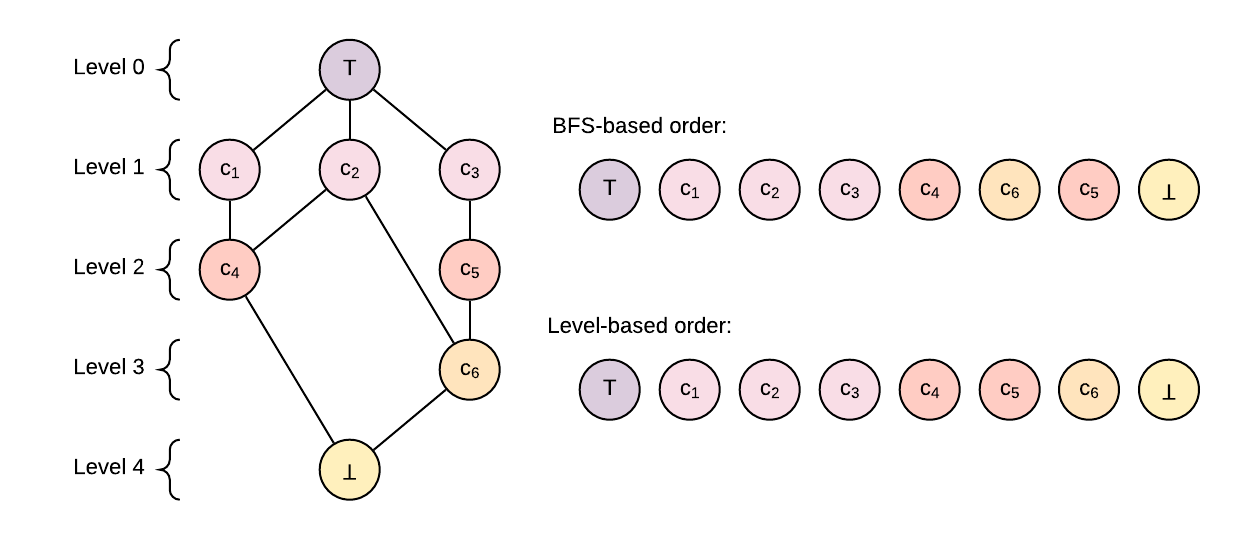
\includegraphics[keepaspectratio, width=.9\textwidth, height=5cm]{Figures/Ch1/example_order.png}
    \caption{Lattice from \cref{fig:hasse} organized in levels and the corresponding level-based and BFS-based orders.}
    \label{fig:level-order}
\end{figure}

Using this new order $\mathcal{O}^L$ with the method of~\cite{graphrnn:2018:jiaxuan} maintains most of the properties demonstrated in~\cite{graphrnn:2018:jiaxuan}.
However, the distance between related nodes (concepts in our case) is less constrained, as concepts of the last layers can be related by $\prec$ with concepts of first layers.
%In practice, this distance between related nodes does not
Conversely, using level-based ordering instead of BFS allows the adjacency vectors to contain only outgoing edges and no incoming ones.
Indeed, for all $c_1, c_2 \in C$ such that $c_1 \prec c_2$, if $c_1 \in l_i$ then $c_2 \in l_j$ with $i < j$.
In other words, a concept is only related to previous elements in the order.

In our example, BFS and level-based ordering produce different results.
Indeed, $c_6$ appears before $c_5$ with BFS, so we need to represent the relation of $c_6$ and $c_5$ with an incoming edge from $c_6$ in the adjacency list of $c_5$.
However, in the level-based ordering $c_6$ appears after $c_5$ and there is no need for incoming edges.

\subsection{Encoding the Lattice Adjacency\label{sec:enc-adjacency}}
%\todo[inline]{The whole subsection is a work in progress}
The lattice adjacency can be encoded in multiple ways.
A first method is to directly consider the sequence of adjacency vectors of different sizes as in~\cite{graphrnn:2018:jiaxuan}.
A second method consists in concatenating the adjacency vectors, and a third method is to use the adjacency matrix as described in the following paragraph.
For practical purposes, we tend to represent the data as vectors or matrices, so we focus on the last two representations.
The concatenation of the adjacency vectors is the most optimal in terms of used space, while the adjacency matrix separates the adjacency of each node across one of the dimensions. The adjacency matrix provides additional benefits, like an easier visualization and simpler manipulation of the adjacency. However, the adjacency matrix requires twice the space of the concatenated adjacency vectors, as the upper triangular matrix is not used.

\subsubsection{Basic Adjacency Matrix}
We define a matrix $\mathbf{L}$ such that the entry at row $i$ and column $j$, $\mathbf{L}_{i,j} = S^{\mathcal{O}L}_{i,j}$, with $S^{\mathcal{O}L}_{i,j}$ the element at position $j$ in $S^{\mathcal{O}L}_i$.
Where $S^{\mathcal{O}L}_{i,j}$ is not defined ($i \leq j$), $\mathbf{L}_{i,j} = 0$.
In other words, we fill a lower triangular matrix with the adjacency vectors.
The resulting lower triangular matrix is the adjacency matrix in the case of $\prec$ and $<$.
For $\leq$, the diagonal ($i = j$) of the matrix of $<$ must be set to 1.

When using a model to predict this matrix, we are in a binary classification problem between two classes: NO EDGE ($0$) and EDGE ($1$).
The model can thus be trained using BCE.

\subsubsection{Adjacency Matrix \emph{à la} Sequence Modeling}
GraphRNN is an architecture designed to process a sequence of nodes, each represented by a sequence of edges.
Traditionally when using RNNs to process sequences we use special values to mark boundaries in the sequence, \eg, the start and end of the sequence.
A special value is also dedicated to padding the sequence. This padding value is used to make the sequence of a batch have the same size.

We also propose to make use of the empty space in the upper triangular matrix.
The transpose of the adjacency matrices of $\prec$, $<$, and $\leq$ are respectively the adjacency matrices of $\succ$, $>$, and $\geq$.
For our triangular matrix containing only outgoing edges from the nodes, the transposed matrix represents the incoming edges.
This transposed matrix is upper triangular, and we use it to fill the unused space of the lower triangular matrix.
Using this construction, we have redundancy between the lower and upper triangular matrices.
This redundancy can prove beneficial for our task, as we can use the upper triangular matrix to check the results of the lower one.

For each node of the graph, we have a sequence of values as follows:
\begin{enumerate}
    \item a \textit{start of sequence} (SOS) value;
    \item the sequence of outgoing edges, either $1$ if there is an edge or $0$ otherwise;
    \item a \textit{middle of sequence} (MOS) value;
    \item the sequence of incoming edges, either $1$ if there is an edge or $0$ otherwise;
    \item an \textit{end of sequence} (EOS) value;
    \item as many \textit{padding} (PAD) values as necessary to reach the size of the largest element in the batch.
\end{enumerate}
We also add sequences full of PAD in the sequence of nodes to reach the size of the largest element in the batch.
The resulting data takes the form of a matrix containing one of 6 values in each entry: NO EDGE ($0$), EDGE ($1$), SOS, MOS, EOS, and PAD.
An example of a batch encoded using this process is shown in \cref{fig:data-pad}.

\begin{figure}
    \centering
    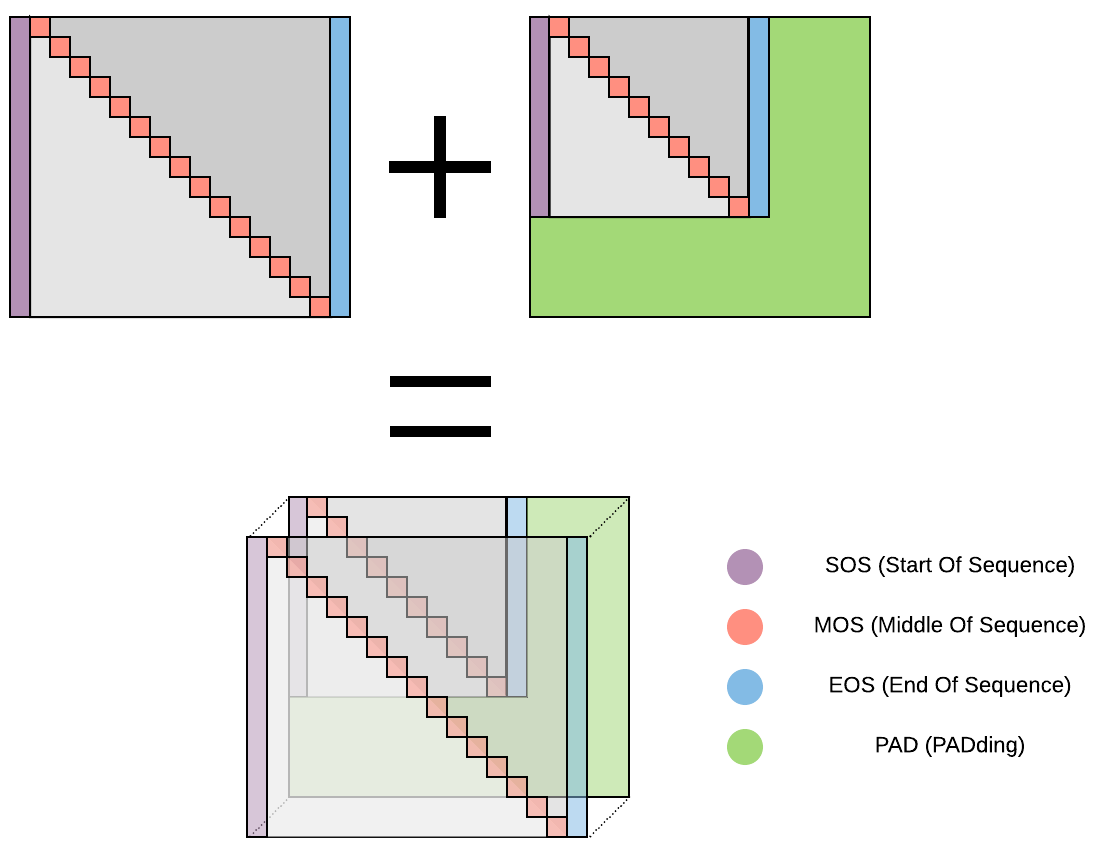
\includegraphics[keepaspectratio, width=.9\textwidth, height=10cm]{Figures/Ch1/pad.png}
    \caption{Diagram of a batch of 2 samples encoded using the 6 values NO EDGE ($0$) and EDGE ($1$) for the adjacency, SOS, MOS, EOS, and PAD.}
    \label{fig:data-pad}
\end{figure}

When using a model to predict this matrix, we are in a multi-label classification problem between 6 classes corresponding to the possible values.
The model can thus be trained using cross-entropy.

\subsection{Encoding the Concepts\label{sec:enc-intents-extents}}
Concepts can be represented using either their intents, their extents, or both.
In FCA, there are two ways to encode the intents and the extents: the \textit{full encoding} and the \textit{narrow encoding}.
Using the full encoding, all the attributes (or objects) of the intent (respectively extent) are used to represent a concept.
The narrow encoding however only use the attributes (or object) that ``appear'' in the concept, in other words, the attributes (respectively objects) that are present in the concept's intent (respectively extent) but not in the ones lower (respectively higher) according to the partial order $\leq$.
To reconstruct the full intent (respectively extent) of a concept from the narrow encoding, we take the set of all the attributes (respectively objects) in the narrow encoding of the concept and the ones of concepts lower (respectively higher) according to $\leq$.
An interesting property of this narrow representation is that each attribute (and object) appear only once in the lattice.
\cref{fig:encoding} shows the narrow encoding of the example lattice from \cref{fig:hasse}.

\begin{figure}
    \centering
    %\includegraphics{}
    %\subcaptionbox{Full encoding ()}{
    %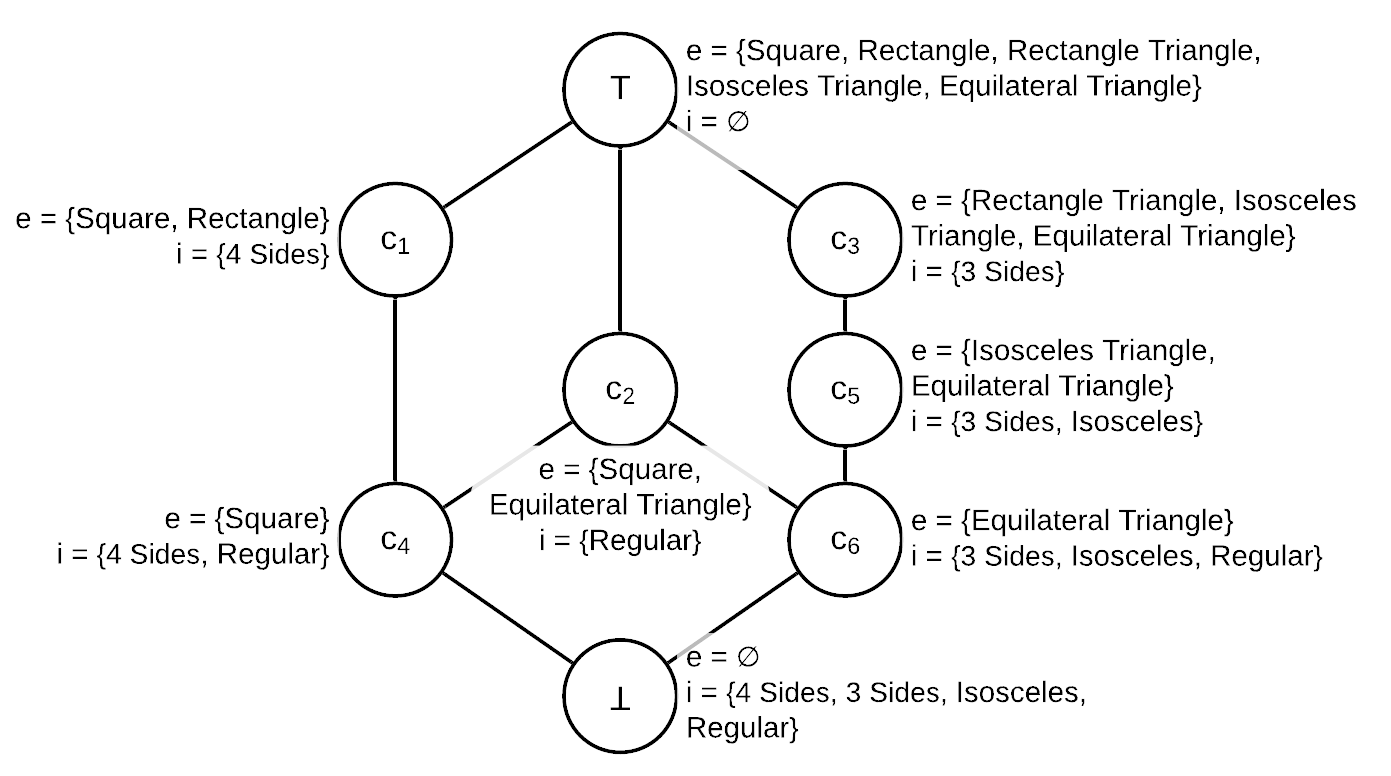
\includegraphics[keepaspectratio, height=8cm, width=.56\textwidth]{Figures/Ch0/example_full.png}}
    %\subcaptionbox{Narrow encoding}{
    %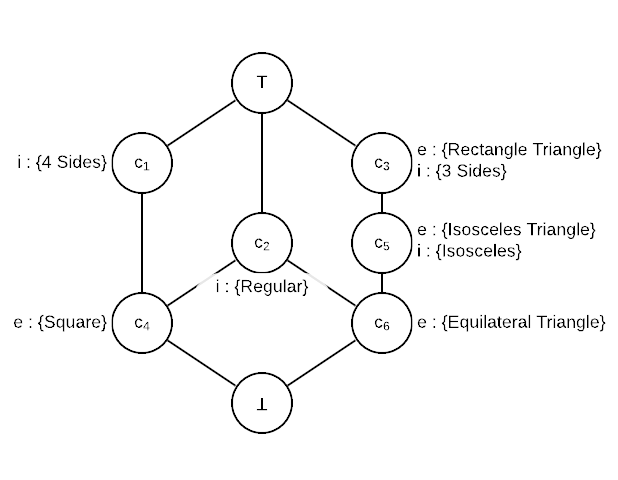
\includegraphics[keepaspectratio, height=8cm, width=.42\textwidth]{Figures/Ch0/example_narrow.png}}
    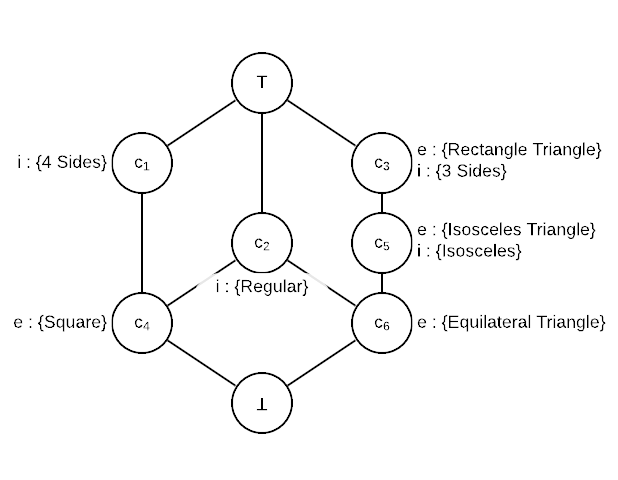
\includegraphics[keepaspectratio, height=7cm, width=.9\textwidth]{Figures/Ch0/example_narrow.png}
    \caption{Narrow encoding of the example lattice of \cref{fig:hasse}.}
    \label{fig:encoding}
\end{figure}

We design two numerical representations for the concepts.
The first one is a matrix based on the full encoding.
The entry at row $i$ and column $j$ is $1$ if the attribute $a_j$ (or object $o_j$) is present in the intent (respectively extent) of the concept indexed $i$ in $\mathcal{O}^L$, and $0$ otherwise.
The second representation is based on the narrow encoding. It takes the form of a vector, with each entry corresponding to an attribute (or object).
The value of an entry is the index in $\mathcal{O}^L$ in which the corresponding attribute (respectively object) ``appears''.



\section{Using GraphRNN for Lattices Modeling\label{sec:graph-model}}

The architecture we propose to model lattices as graphs is an implementation of GraphRNN as a constrained VAE.
We first detail the workings of the original GraphRNN in \cref{sec:graph-model-graphrnn} and then present our adapted architecture in \cref{sec:graph-model-full}. 

\subsection{GraphRNN\label{sec:graph-model-graphrnn}}
This subsection is a quick overview of the inner workings of GraphRNN. For a detailed explanation, see~\cite{graphrnn:2018:jiaxuan}.

GraphRNN is a model for graph modeling composed of 2 components:
a \textit{graph-level} GRU to generate nodes, and a \textit{node-level} GRU to generate edges.
For each step of the graph-level model, the node-level model generates the edges with the previous nodes in the sequence.
In other words, the node-level model predicts the adjacency vector $S^\pi_i$ described in \cref{sec:level-order}.
The adjacency vector predicted by the node-level model is taken into account for the next step of the graph-level model.
The model can be considered in two phases: training and inference. They respectively correspond to training the model and using the model to generate new graphs.

In practice, the graph-level model generates a representation of a node's adjacency at each step, as a fixed-sized vector serving to initialize the node-level model.
This node representation is used as the first hidden state of the node-level RNN.
At each step, the node-level model predicts the probability of an edge existing between the currently processed node and one of the previous nodes.
During inference, this probability is used to randomly sample the edge, which is then used as the input of the next step of the node-level model.
During training the true previously edge is used instead.
\cref{fig:graphrnn} is an example of how the model unfolds when during inference.

The TensorFlow (an alternative to PyTorch) implementation of GraphRNN is available in the Snap Stanford repository\footnote{\url{https://github.com/snap-stanford/GraphRNN}}.

\begin{figure}
    \centering
    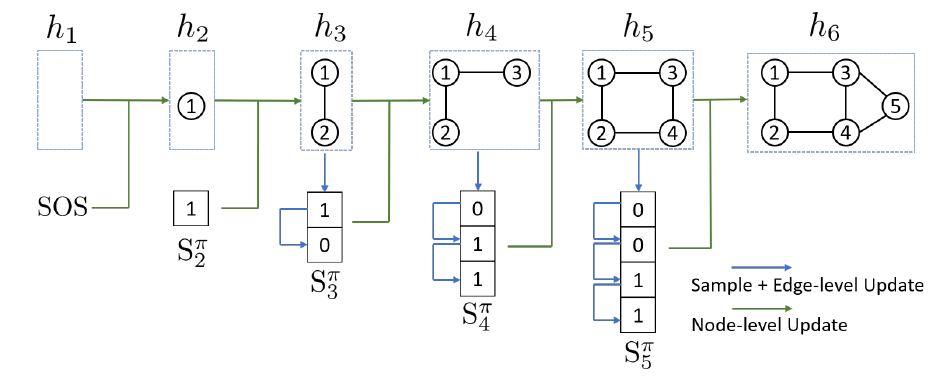
\includegraphics[keepaspectratio, width=.9\textwidth, height=4cm]{Figures/Ch1/graphrnn.png}
    \caption{GraphRNN at inference time. Figure 1 from~\cite{graphrnn:2018:jiaxuan}.}
    \label{fig:graphrnn}
\end{figure}

\subsection{GraphRNN Constrained VAE\label{sec:graph-model-full}}
%\todo[inline]{the planned setup, with intent/extent modeling}

To have a model able to generate lattices from FC based on the graph structure of the lattice, we decide to split the problem.
The first half of the problem is to learn a way to accurately represent lattices in a way that can be used to decode them.
For that, we use an auto-encoder architecture to learn an embedding of lattices, and in particular a VAE.
Indeed, as mentioned in \cref{sec:vae}, VAEs are more suited to generation problems like ours than traditional auto-encoders because of the properties of the embedding space.
Once we have a representation of lattices, we can tackle the second half of the problem: to use an FC together with the decoder half of the VAE to generate the lattice corresponding to the FC.
In practice, we have 2 main methods to achieve this.
On the one hand, we can use an additional model to generate an embedding of the FC in the same embedding space as the lattices.
On the other hand, we can use a constrained VAE with the FC as the condition.
With this second option, the condition can contain other information in addition to the one from the FC, and the FC embedding is not necessarily in the lattices' embedding space, making it a more favorable option. However, the core of the problem stays the same: we need an embedding of the FC.
The whole pipeline is schematized in \cref{fig:graphrnn-cvae}.

\begin{figure}
    \centering
    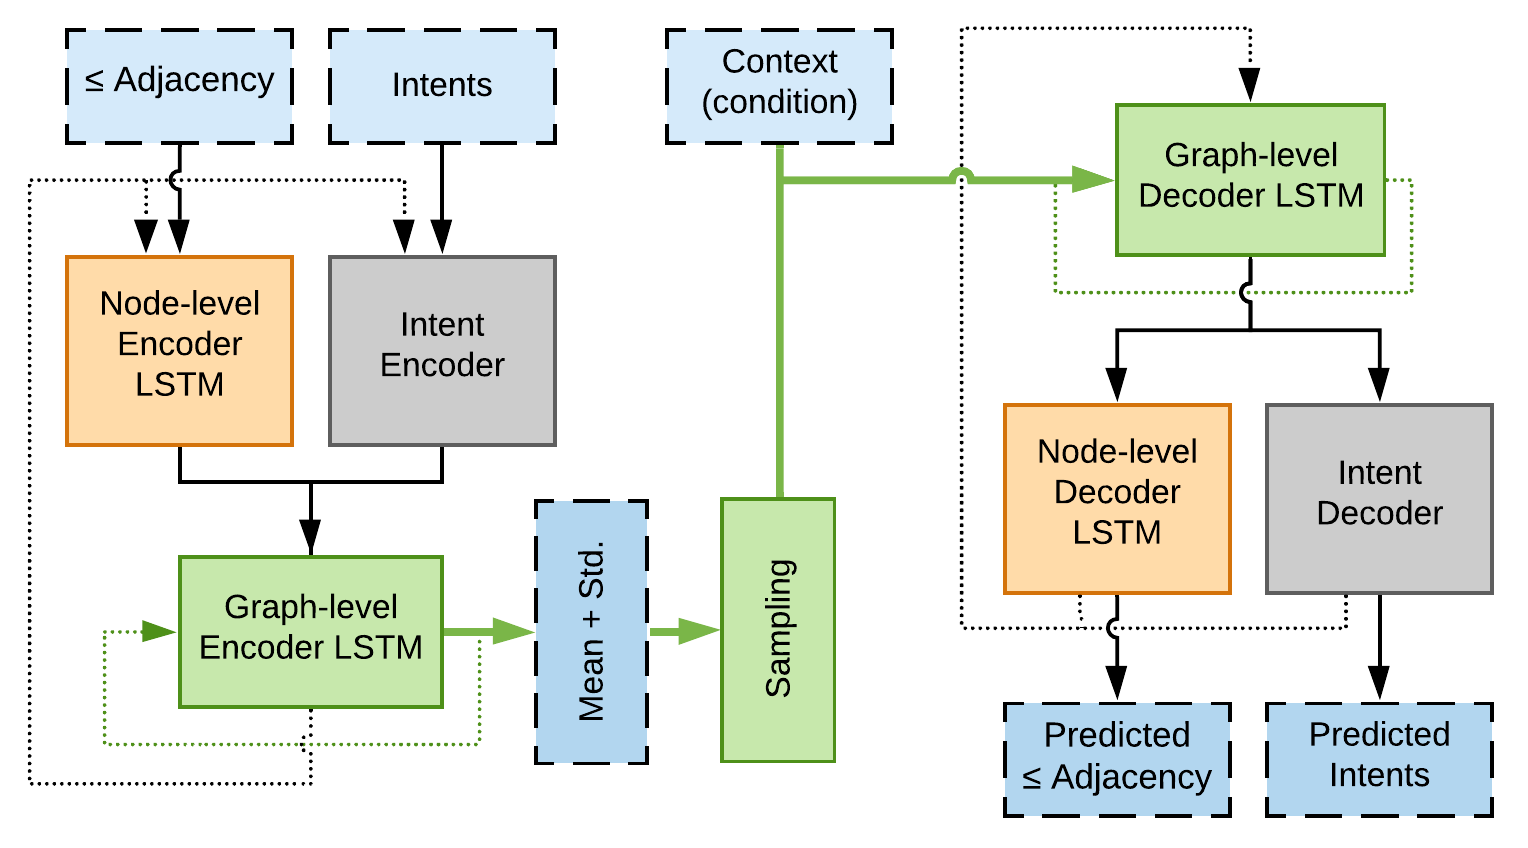
\includegraphics[keepaspectratio, width=.9\textwidth]{Figures/Ch1/grnn_full_.png}
    \caption{Adapted GraphRNN Constrained VAE.}
    \label{fig:graphrnn-cvae}
\end{figure}

The development plan is in 3 steps: \textit{(i)} building a VAE for lattices using the original GraphRNN design, \textit{(ii)} integrating the intent generation to the VAE, by extending the original GraphRNN design and \textit{(iii)} integrate the condition system.
The first two steps of the approach allow our model to first learn the representation of lattices in an auto-supervised manner, thanks to the auto-encoding principle.
At the issue of those two steps, the model should have learned ``what is a lattice''.
The third step is for developing the embedding of the FC.
This development process allows us to adapt the approach if one of the steps do not provide acceptable results.
Indeed, if the model does not manage to capture the basic structural properties of lattices (without the intents), it is unlikely that it will be able to handle the full complexity of the structure of lattices with the intents.
Similarly, if the model has trouble handling the full complexity of lattices, we won't be able to use it to generate lattices from FCs.


Our auto-encoder is composed of two GraphRNNs, one for the encoder and the other for the decoder.
The encoder GraphRNN reads the graph, and the last hidden state of the graph-level RNN is used to build the embedding.
The decoder GraphRNN is initialized with the embedding as the first hidden state of the graph-level RNN and generates.
To handle the concept intents, an intent model is added alongside the node-level model.
Similarly to the node-level, this second model takes the output of the graph-level model as its input.
Block diagrams of the folded encoder and decoder are shown in \cref{fig:graphrnn-autoencoder}.

%For the auto-encoder, we decided to share the parameters of the node-level RNN\todo{why?}

\begin{figure}
    \centering
    \subcaptionbox{Encoder\label{fig:graphrnn-encoder}}{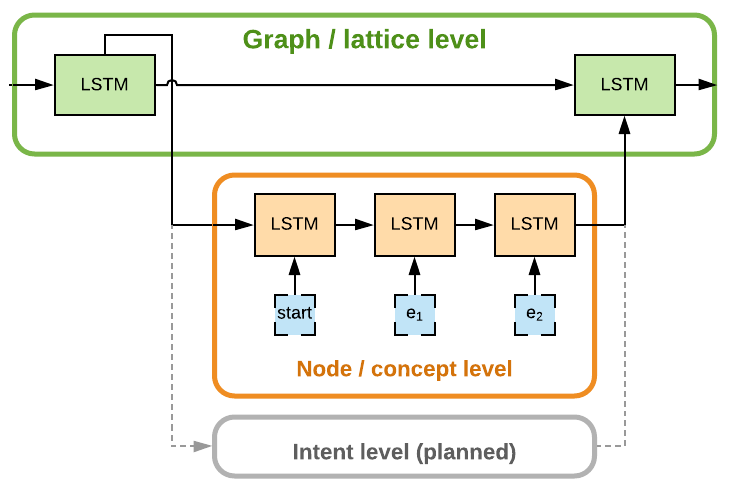
\includegraphics[keepaspectratio, width=.48\textwidth]{Figures/Ch1/grnn_encoder.png}}
    \subcaptionbox{Decoder\label{fig:graphrnn-decoder}}{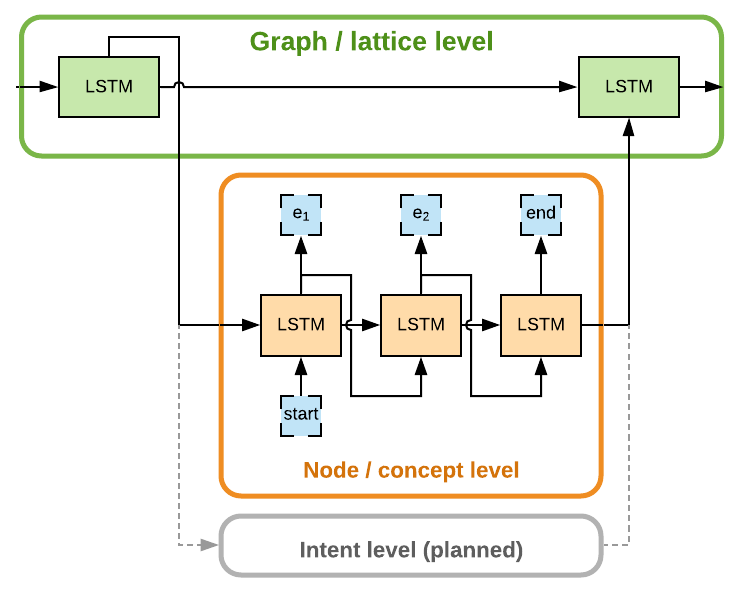
\includegraphics[keepaspectratio, width=.48\textwidth]{Figures/Ch1/grnn_decoder.png}}
    \caption{Details of the adapted GraphRNN, with edge and intent generation.}
    \label{fig:graphrnn-autoencoder}
\end{figure}

\section{Preliminary Experiments and Change of Approach\label{sec:graph-expe}}
To determine the feasibility of the proposed architecture, we first experimented with the reconstruction performance of our VAE without node features, in other words without intent.

\subsection{Reconstruction Performance Without Features}
On a few samples of small size, the reconstruction performance of the VAE was satisfying. 
Examples of reconstructions an early stage proof of concept model are shown in \cref{fig:graph-reconstruction}. This proof of concept model was trained on less than 20 samples smaller than 5 objects and attributes.
However, the prediction performance on our larger dataset described in \cref{sec:data-generation} is not as good.
We experimented with various variants of the model, but without major improvement in the performance.
Those changes include, but are not limitted to, predicting $\leq$ or $\prec$, completely sharing the parameters of the decoder and the encoder, and pretraining.
The performance on the development set of our best model, detailed in \cref{tab:graphrnn-perf}, stays relatively low, with an average F1 score of $0.13$ at best when reconstructing the graph of $\prec$.

\begin{figure}
    \centering
    \subcaptionbox{Prediction}{$\begin{bmatrix}
2 & 3 & 1 & 1 & 0 & 0 & 0 & 0 & 4\\
2 & 1 & 3 & 0 & 1 & 0 & 1 & 0 & 4\\
2 & 1 & 0 & 3 & 0 & 1 & 0 & 0 & 4\\
2 & 0 & 0 & 1 & 3 & 1 & 0 & 0 & 4\\
2 & 0 & 0 & 1 & 0 & 3 & 0 & 1 & 4\\
2 & 0 & 1 & 0 & 1 & 0 & 3 & 1 & 4\\
2 & 0 & 0 & 0 & 0 & 1 & 1 & 3 & 4
    \end{bmatrix}$}
    \subcaptionbox{Gold (expected output)}{$\begin{bmatrix}
2 & 3 & 1 & 1 & 0 & 0 & 0 & 0 & 4\\
2 & 1 & 3 & 0 & 0 & 0 & 1 & 0 & 4\\
2 & 1 & 0 & 3 & 1 & 1 & 0 & 0 & 4\\
2 & 0 & 0 & 1 & 3 & 0 & 1 & 0 & 4\\
2 & 0 & 0 & 1 & 0 & 3 & 0 & 1 & 4\\
2 & 0 & 1 & 0 & 1 & 0 & 3 & 1 & 4\\
2 & 0 & 0 & 0 & 0 & 1 & 1 & 3 & 4
    \end{bmatrix}$}
    \subcaptionbox{Legend}{~~$
    \begin{matrix}
        0:& \text{NO EDGE}\\
        1:& \text{EDGE}\\
        2:& \text{SOS}\\
        3:& \text{MOS}\\
        4:& \text{EOS}\\
        5:& \text{PAD}
    \end{matrix}
    $}
    \caption{Example of lattice reconstruction in the early stages.}%Legend: $0$: NO EDGE; $1$: EDGE; $2$: SOS; $3$ MOS; $4$: EOS; $5$: PAD.
    \label{fig:graph-reconstruction}
\end{figure}

It is hard to compare those results with those presented in~\cite{graphrnn:2018:jiaxuan} as we do not use the same evaluation tools.
Indeed, GraphRNN is evaluated in~\cite{graphrnn:2018:jiaxuan} by comparing structural statistics of predicted graphs with those of true graphs of the modeled family.
Conversely, because our goal is to correctly reconstruct a specific lattice and not any lattice-like graph, we use measures of prediction performance, \eg, the F1 score.
However, given the performance of GraphRNN demonstrated in~\cite{graphrnn:2018:jiaxuan}, we expected higher reconstruction performance, with an F1 score above $0.7$ at least.

\begin{table}
\centering
\begin{tabular}{lrrrr}
\toprule
Relation & Accuracy & Precision &   Recall &       F1\\
       \midrule
$\prec$ & 0.80 $\pm$ 0.05 &  0.50 $\pm$ 0.55 & 0.078 $\pm$ 0.089 & 0.13 $\pm$ 0.15\\
$\leq$  & 0.72 $\pm$ 0.03 &  0.50 $\pm$ 0.55 & 0.046 $\pm$ 0.055 & 0.084 $\pm$ 0.100\\
\bottomrule
\end{tabular}
\caption[Prediction performance of the GraphRNN VAE on the development set, for the adjacency matrices of the graphs of $\prec$ and $\leq$.]{Prediction performance of the GraphRNN auto-encoder, for adjacency matrices of the graphs of $\prec$ and $\leq$. The prediction performance for entries is reported (mean $\pm$ std.).}
\label{tab:graphrnn-perf}
\end{table}

\subsection{Formal Concept Representation and Change of Approach}
To generate the lattice from the FC we decided to add a condition to our VAE.
Ideally, this condition should be the FC in some form. Because the usual constrained VAE architecture requires fixed-sized condition vectors, the representation of the FC has to be of fixed size for any FC.
We could then generate the concept lattice using exclusively the FC as the input, by using some default embedding instead of the output of the encoder.
This process can be seen as being able to generate any lattice, and using the condition to specify which lattice we want: the one corresponding to our FC.
Another option would have been to generate lattice embedding from the FC, in the embedding space defined by our GraphRNN VAE.

Obtaining a detailed enough representation of the complexity of the FC is challenging, because the information defining the lattice is not directly accessible.
Additionally, we have constraints on the size of the representation due to our needs.
Focusing on this problem led us to design BoA presented in \cref{ch:boa}.
The results of the BoA model together with the poor performance of the basic auto-encoder led us to modify our lattice approach.
The new approach is detailed in \cref{ch:intents}.


\chapter{Bag of Attributes: Embeddings for Formal Contexts\label{ch:boa}}


It is essential to represent FCs, to reproduce FCA using neural networks.
Ideally, we want to have a general embedding framework for FCs capable of handling data of arbitrary dimensions while encoding much of the contextual information.

FCA2VEC~\cite{fca2vec:2019:durrschnabel} is, to our knowledge, the only framework to generate embeddings of objects and attributes from an FC. This approach, which we explain in \cref{sec:fca2vec}, has several limitations.
Firstly, the embeddings for objects and attributes are not defined in the same embedding space, which can be problematic when processing objects and attributes together. Secondly, the embedding models need to be trained separately on every processed FC, which is costly. Thirdly, there is no guaranty that the resulting embeddings can be used to generalize across FCs, which is blocking for our goal of developing a single model able to handle FCs.

To overcome these limitations, we propose an embedding framework for FCs.
As mentioned in \cref{sec:problem}, we focus on attributes and intents.
To design this framework, we asked ourselves what attributes are, and in particular, which aspects of the attributes should interest us to reproduce FCA.
We decided to focus on how attributes interact with each other, and more precisely, which attributes appear together and how often.
This answer is based on the following observation: attributes that always appear together in the same dataset appear in the same intents, in the same concepts.
%Our answer is based on the observation that attributes that always appear together in the same dataset appear in the same intents, in the same concepts.
%We are interested in how attributes interact with each other, and more precisely, which attributes appear together and how often.
However, we are not interested in the order of the attributes, because changing said order in an FC will not change the resulting lattice.

We detail the resulting architecture, \textit{Bag of Attributes} (BoA), in \cref{sec:boa}, and present experimental results in \cref{sec:boa-expe}.
BoA is the object of an article~\cite{boa:2020:marquer} published in the 8th FCA4AI (``What can FCA do for Artificial Intelligence?'') workshop\footnote{\url{https://fca4ai.hse.ru/2020/}}. A significant portion of the content of this section is a reformulation of the article~\cite{boa:2020:marquer}.

\section{State of the Art: FCA2VEC\label{sec:fca2vec}}

Binary FCs are binary tables. There exist a wide variety of \textit{rank lowering} methods to represent such tables, like \textit{latent semantic analysis} in NLP.
The resulting representation is usually a pair of sets of vectors, one for the rows and one for the columns of the table.
However, such methods do not take into account the properties manipulated by FCA, such as the closure operator or the formal concepts.

To our knowledge, the only embedding framework specialized for FCs and based on FCA is FCA2VEC~\cite{fca2vec:2019:durrschnabel} by  Dürrschnabel \etal{}.
We explain the major aspects of their approach in this section. For further detail, see the original article.
In \cref{sec:fca2vec-o2v} and \cref{sec:fca2vec-c2v}, we describe the embedding architectures based on FCA's closure operator proposed in~\cite{fca2vec:2019:durrschnabel}, namely \textit{object2vec}, \textit{attribute2vec}, and \textit{closure2vec}.
Finally, we describe in \cref{sec:fca2vec-evaluation} the methods used in the article to evaluate {object2vec} and {attribute2vec}.
Note that all FCA2VEC models are designed to build embeddings of small dimensions (2 or 3 elements only).

\subsection{{Object2vec} and {Attribute2vec}}\label{sec:fca2vec-o2v}
\textit{Object2vec} and \textit{attribute2vec} are proposed in FCA2VEC to provide embeddings of objects and attributes using respectively the extents and the intents.
They are based on the idea \blockcquote{fca2vec:2019:durrschnabel}{to interpret two objects to be more close to each other if they are included in more concept extents together.}

Based on this principle, the authors adapt the \textit{word2vec}~\cite{word2vec:2013:mikolov} distributional word embedding framework.
{Word2vec} learns to associate a word with the words it appears with often, by learning to predict either the context of a word given the word (\textit{skip-gram} variant) or a word based on its context (\textit{CBoW} variant). This principle is schematized in \cref{fig:w2v}.
By interpreting the objects as words and the extents as sentences and applying {word2vec}, an object will be associated with objects often appearing in the same extent. The resulting model is called {object2vec}.
Similarly, {attribute2vec} is obtained by using attributes as words and intents as sentences. 

\begin{figure}
    \centering
    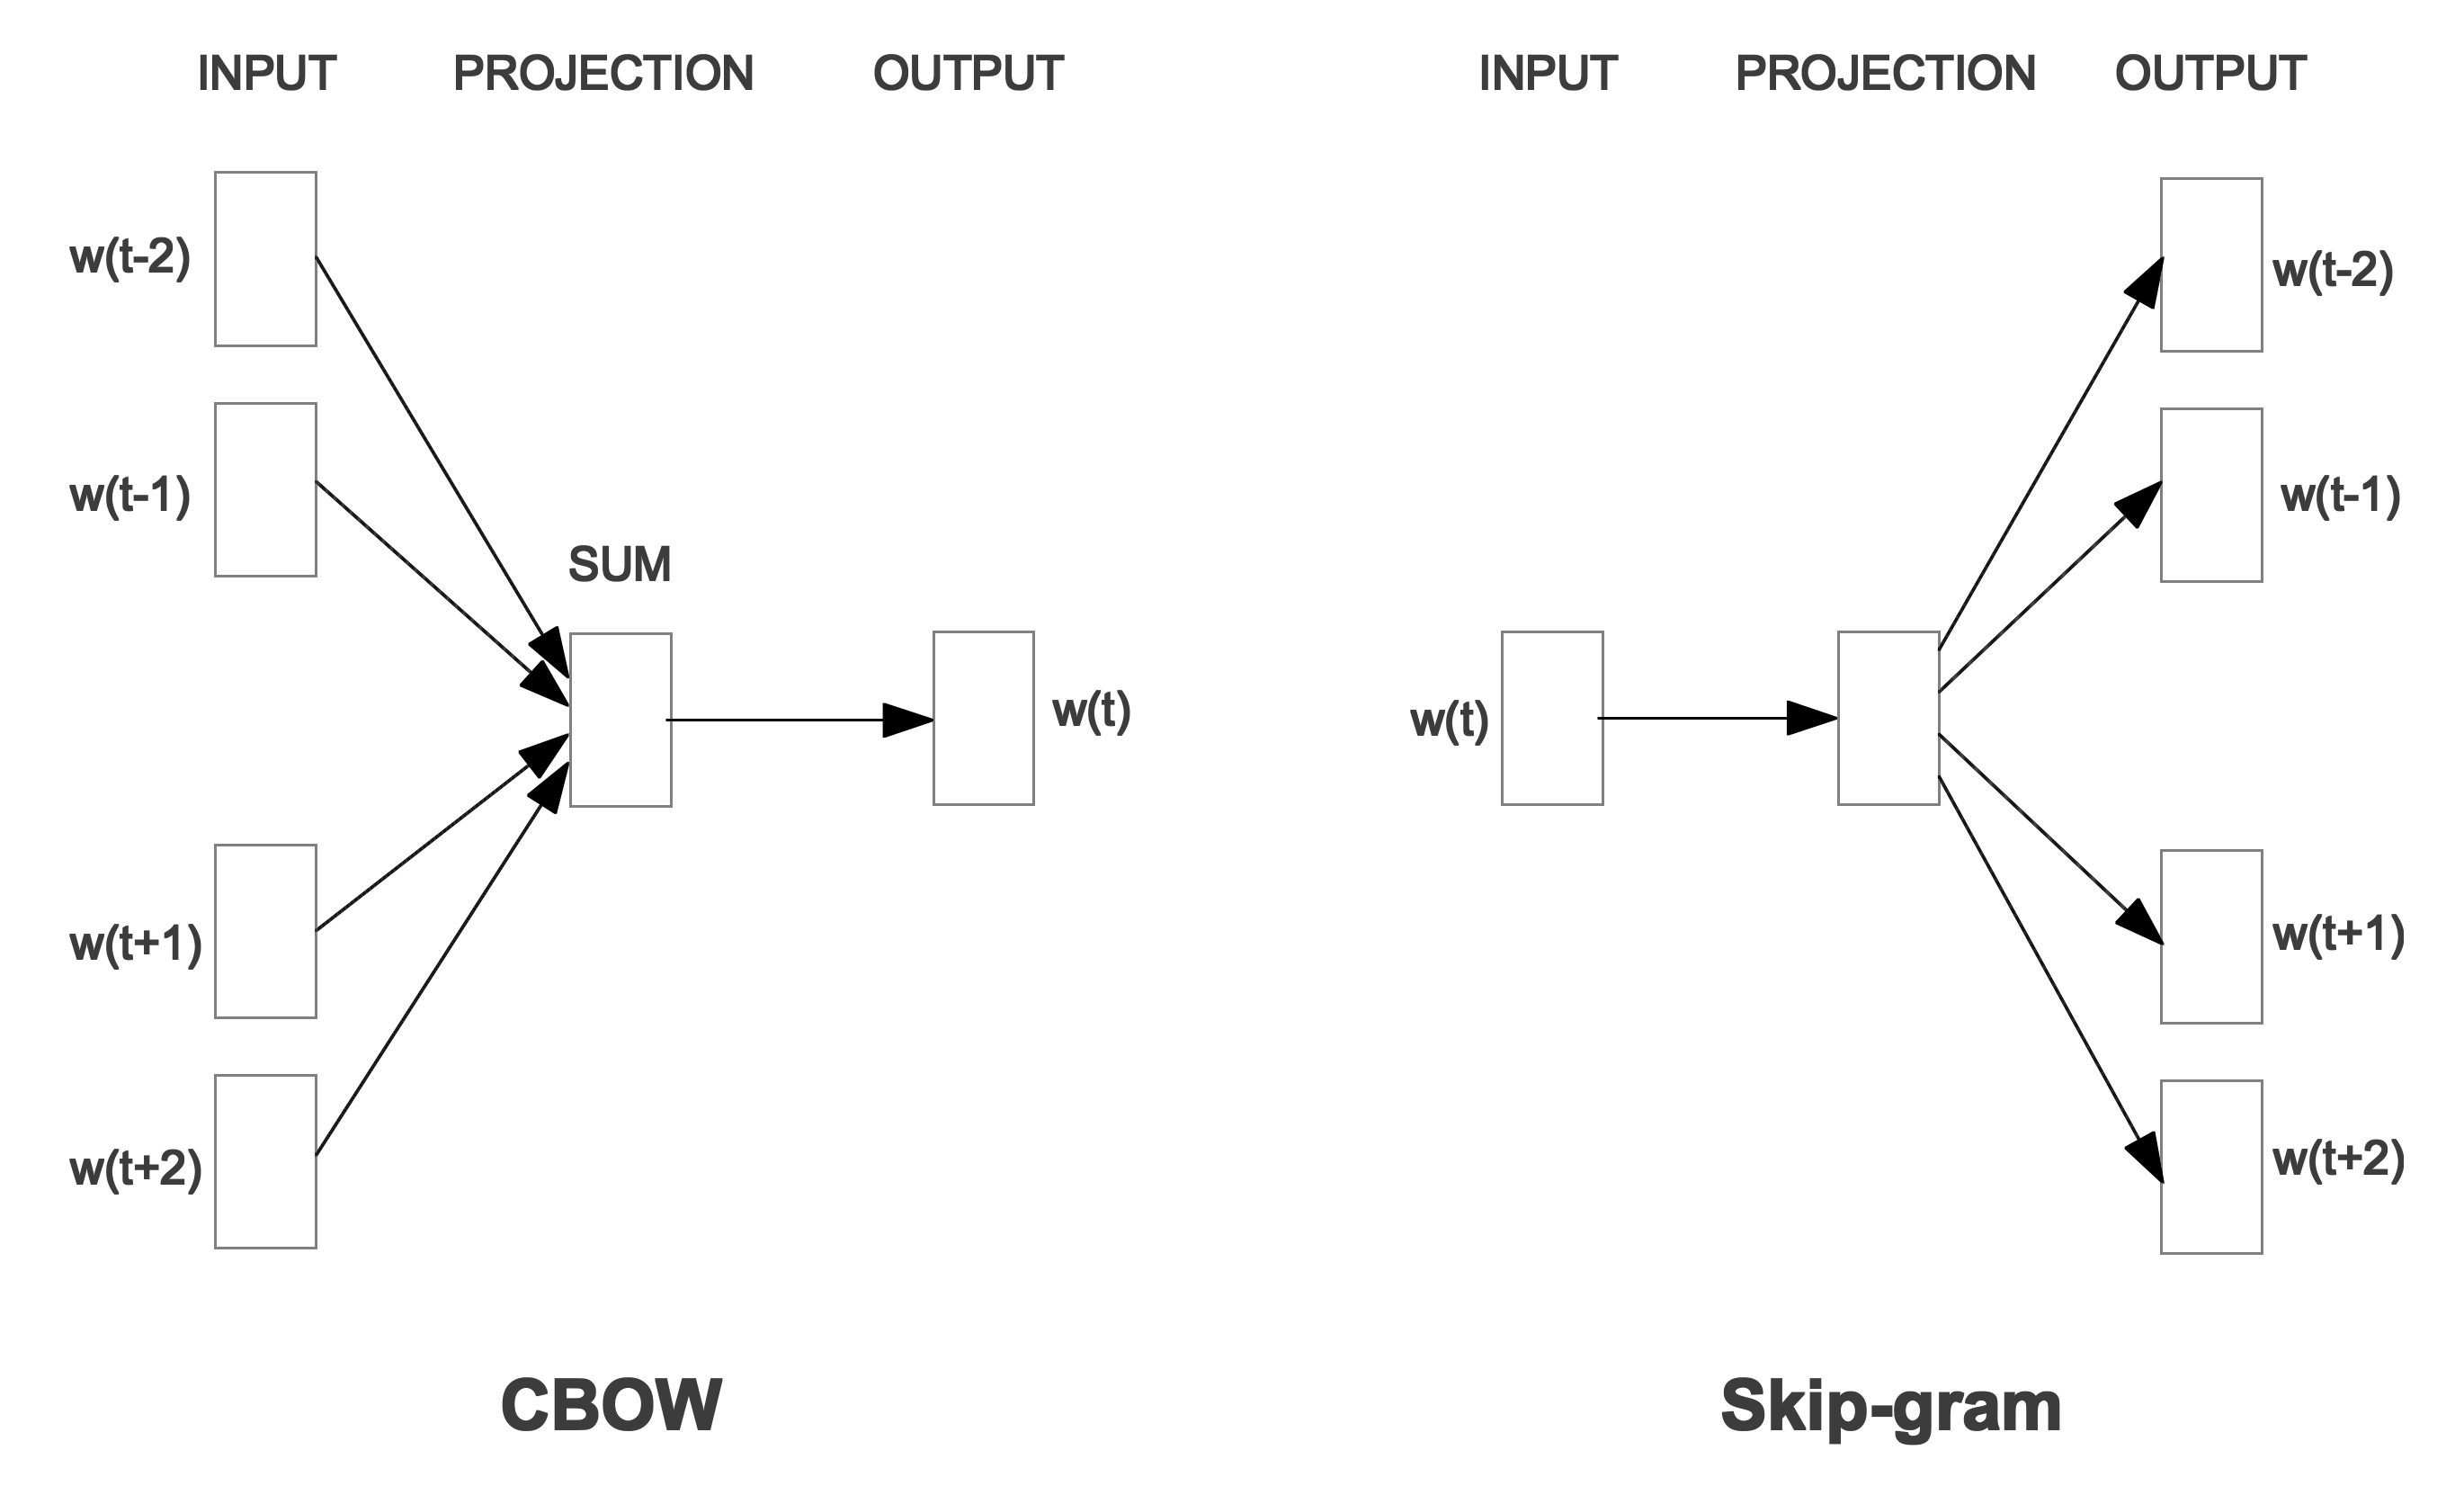
\includegraphics[width=.9\textwidth, height=5cm, keepaspectratio]{Figures/Ch2/word2vec.png}
    \caption{Continuous Bag of Words (CBoW) and skip-gram architectures from word2vec. Figure 1 from \cite{word2vec:2013:mikolov}.}
    \label{fig:w2v}
\end{figure}

The samples used to train {object2vec} are generated by taking, for each extent $e$, for each object $o_1\in e$, either:
\begin{itemize}
    \item all the pairs $\langle o_1, o_2 \rangle$ for all the other objects $o_2$ in the extent ($o_2 \in e/o_1$\footnote{As a reminder, $e/o_1$ stands for the set $e$ without the element $o_1$.\label{fn:e-less-o}}), for the {skip-gram} variant;
    \item the pair $\langle e/o_1, o_1 \rangle$, for the {CBoW} variant.
\end{itemize}
In practice, $o_1$ and $o_2$ are represented by their respective one-hot encoding, and $e/o_1$ is represented by the element-wise average vector of the one-hot encoding of its elements.

It is interesting to note that for an extent of size $|e| = 5$, 5 samples are generated for {CBoW}, while for {skip-gram} $5\times 4$ (2 among 5) samples are generated. For FCs with large amounts of objects and concepts, the number of samples used to train the {skip-gram} variant is explosively large using this method.

\subsection{Closure2vec}\label{sec:fca2vec-c2v}
\textit{Closure2vec} is proposed in FCA2VEC based on the result of~\cite{encoding:2007:rudolph}.
Rudolph demonstrates that for any closure operator on two sets $X$ and $Y$, there exists an MLP able to perfectly encode said closure operator.
The MLP of the closure operator from $X$ to $X$ has an input size of $|X|$, a first layer with $|Y|$ neurons and a second one with $|X|$ neurons.
This general result is applicable to FCA's closure operator, \eg, $\cdot''$ on the set of attributes can be encoded with a 2 layer MLP with an input size of $|A|$, a first layer with $|O|$ neurons and a second one with $|A|$ neurons.
Such a model, once defined, can be learned using deep learning algorithms.

{Closure2vec} is designed to take two sets of attributes (for example, two objects) and compute an embedding for each of them.
It is then trained to match the \textit{closure Hamming distance} (see \cref{def:chd}) between the two sets of attributes to the distance between the corresponding embeddings. The distance between the embeddings is computed using either the Euclidian or the cosine distance.
In practice, {closure2vec} uses a 2 layer MLP as defined in~\cite{encoding:2007:rudolph}, with an additional feed-forward layer that computes a 2- or 3-dimensional embedding vector.

\begin{definition}\label{def:chd}
The \emph{closure Hamming distance} (CHD) between two sets of attributes is the \emph{Hamming distance} between the binary representation of respective closures of the two sets of attributes. In other words, it is the number of modifications necessary to go from one closure to the other.
Two attribute sets are called \emph{equivalent} if they have the same closure, so if their CHD is 0.
\end{definition}

{Closure2vec} is trained on randomly sampled pairs of sets of attributes, with the sets in a pair differing by exactly one attribute.

\subsection{Evaluation}\label{sec:fca2vec-evaluation}
In this subsection, we describe the evaluation processes used to evaluate {attribute2vec} and {object2vec}.
For the evaluation, the authors use real-world datasets and tasks using the embeddings.

%For \textit{closure2vec}, the authors evaluate the CHD between the intents of the concepts of the wiki44k and the Mushroom datasets.

\begin{table}
    \centering
    \begin{tabular}{lllll}
    \toprule
    Dataset & \# Objects & \# Attributes & Density & \# Concepts\\
    \midrule
    ICFCA$^\star$ & 263 & 8442 & 0.005 & 680 \\
    Wiki44k & 45021 & 101 & 0.04 & 21923\\
    \bottomrule
    \end{tabular}
    \caption{Descriptive statistics on ICFCA$^\star$ and wiki44k, the datasets used to evaluate {object2vec} and {attribute2vec}. Table 1 from~\cite{fca2vec:2019:durrschnabel}.}
    \label{tab:fca2vec-datasets}
\end{table}

\subsubsection{Attribute Clustering for Attribute2vec\label{sec:fca2vec-clustering}}
The performance of \textit{attribute2vec} is evaluated through an attribute clustering task.
The \textit{wiki44k} dataset\footnote{Available at \url{http://people.mpi-inf.mpg.de/~gadelrab/RuLES/}.} is used for this experiment. 
Wiki44k is a knowledge graph (KG) where \textit{entities} (the nodes) are put in relation using \textit{statements} (directed labeled edges) labeled with \textit{properties} (edge labels).
The corresponding FC uses the entities as objects and property names as attributes. An object $o_i$ and an attribute $a_j$ are related by the incidence relation if entity $o_i$ appears in a statement labeled with property $a_j$.
As the authors of~\cite{fca2vec:2019:durrschnabel} mention, wiki44k is sparse for an FC, with a density of 0.04.

The canonical base of wiki44k is used for the attribute clustering task of~\cite{fca2vec:2019:durrschnabel}.
A canonical base can be seen as a minimal set of implications (of the form $X\rightarrow Y$, with $X, Y\in A$) which is sufficient to describe all the valid implications of a lattice.
An implication $X\rightarrow Y$ is valid if $Y$ appears every time $X$ does, \ie, if we have $X$, we always have $Y$.
Hanika, one of the authors of~\cite{fca2vec:2019:durrschnabel}, explains in~\cite{wiki44k-tr:2019:hanika} the interest of studying the canonical base of the FC of wiki44k. For further detail on the canonical base see, \eg, \cite{canonical:2016:karell,wiki44k-tr:2019:hanika}.

The attribute clustering task consists in clustering attribute embeddings using a simple clustering algorithm (k-means).
The performance is measured by taking the rate of \textit{intra-cluster} implications, \ie, implications from the canonical base which are \blockcquote{fca2vec:2019:durrschnabel}{completely contained in one cluster}. An implication $X \rightarrow Y$ is called \textit{intra-cluster} if there is a cluster $K$ such that $X \cup Y \in K$.
Two baselines are used: \textit{(i)} a random clustering, obtained by generating random clusters with similar sizes as ones obtained by {attribute2vec}, and \textit{(ii)} a naive clustering, obtained by clustering a naive representation of the attributes. For an attribute $a$, this naive representation is the binary encoding of $a'$, the set of objects having the attribute $a$.

The performance reported in~\cite{fca2vec:2019:durrschnabel} is shown in \cref{tab:fca2vec-a2v-perf}.
The performance of {attribute2vec}'s CBow variant is lower than the random baseline, so the corresponding results are not reported by~\cite{fca2vec:2019:durrschnabel}. 
{Attribute2vec} skip-gram outperforms the two baselines, which could be expected given the training objective of attribute2vec.
Indeed, attribute2vec is trained to bring together attributes often appearing in the same intents, and implications describe sets of attributes appearing together in the dataset.

\begin{table}
    \centering
    \begin{tabular}{rllll}
    \toprule
    Emb. size & Model & $k = 2$ & $k = 5$ & $k = 10$ \\
    \midrule
    & Naive & $0.0158\pm0.0000$ & $0.0055\pm0.0042$ & $0.0035\pm0.0002$\\
    \midrule
    \multirow{2}{*}{2} & Random & $0.0534\pm0.0412$ & $0.0084\pm0.0088$ & $0.0010\pm0.0007$ \\
    & a2v-SG & $0.1608\pm0.0031$ & $0.0703\pm0.0122$ & $0.0069\pm0.0004$ \\
    \midrule
    \multirow{2}{*}{3} & Random  & $0.0219\pm0.0107$ & $0.0036\pm0.0027$ & $0.0007\pm0.0004$ \\
    & a2v-SG & $0.3217\pm0.0005$ & $0.1038\pm0.0218$ & $0.0080\pm0.0001$ \\
    \bottomrule
    \end{tabular}
    \caption{Rate of intra-cluster implication with the {attribute2vec} skip-gram variant (\textit{a2v-SG}) and the {naive} and {random} baselines, for embeddings of size 2 and 3, for $k=2$, $5$ and $10$ clusters, for 20 repetitions of the evaluation experiment (mean $\pm$ std.). Table 3 from~\cite{fca2vec:2019:durrschnabel}.}
    \label{tab:fca2vec-a2v-perf}
\end{table}

% Dataset:
% - wiki44k (http://people.mpi-inf.mpg.de/~gadelrab/RuLES/), from "rule learning from knowledge graphs guided by embedding models", adapted by "Discovering Implicational Knowledge in Wikidata"
% - wiki44k cannonical base for score computation

% > For comparison, we have also included the data set wiki44k as provided by [15], a small subset of simple statements extracted from a Wikidata dump from December 2014. Meanwhile, though, the usage of some properties on Wiki-data has changed, and, in particular, eight properties usedin this data set have since been deleted on Wikidata. Hence, we have also generated wiki44k-tr,where these properties have been replaced by their modern equivalents:
% - P7(“brother”), P9 (“sister”): replaced by P3373 (“sibling”)
% - P45 (“grandparent”): replaced by P1038 (“relative”) with a P1039 (“type of kinship”) qualifier with value Q167918 (“grandparent”)
% - P70 (“order”): replaced by P171 (“parent taxon”), where the object gets an additional P105 (“taxon rank”) statementwith value Q36602 (“order”),
% - P71 (“family”): replaced by P171 (“parent taxon”);where the object gets an additional P105 (“taxon rank”) statement with valueQ35409 (“family”),
% - P107 (“main type GND”), P132 (“administrative entity”):replaced by P31 (“instance of”), and
% - P133 (“language family”): replaced by P279 (“subclass of”).
% Both data sets were converted to JSON formatand then processed analogously to the other data sets. Data sets wiki44k-2018 and wiki44k-2018-tr are subsets of the 2018 dump obtained by dropping all items and properties (and statements connecting those) not appearing in wiki44k and wiki44k-tr, respectively.

% properties

% Their pipeline:
% 1. Applying attribute2vec on wiki44k (lr=1.0, ~5 epochs)
% 2. K-means clustering of embeddings (Sklearn, k-means++, the default), with k=2, k=5, k=10
% 3. Intra-cluster implications:
% %    > An implication drawn from the canonical base, i.e., A→B ∈ L, is called intra-cluster if there is some c∈C such that A∪B⊆c. The canonical base of wiki44k has the size 7040.For a clustering C we compute the ratio of intra-cluster implications.
% %    > Definition 11 (Canonical basis [30]). The canonical basis Σ_{cb} on S is defined by:
% %    Σ_{cb} = {B → φ(B) \ B : B ⊆ S is a pseudo-closed set of φ}
% %    where a subset B of S is pseudo-closed when B is not closed (i.e. B 6= φ(B)), and φ(B') ⊂ B for every pseudo-closed B' ⊂ B.

% 4. repeat 1/2/3 20 times
% 5. baseline:
%     - random clustering of attribute set
%     - "naive" clustering: attribute m represented by one-hot encoding of objects, then k-means

% Canonical basis from lattice:
% 1. before all: 
%     The canonical basis cannot be directly obtained with a lattice L as input.
% %    One needs to compute an IS Σ representing L before computing the canonical basis of Σ with the previous treatment.
% %    In [49], the following IS Σ defined on J_{L} is stated to characterize L:
% %        Σ = {J_{x} + j → J_{xVj} : x ∈ L, j ∈ JL , j 6≤ x and J_{x} + j not closed}
% %2. First, apply the right maximal transformation by replacing the conclusion of each rule X → Y by φ(X) \ X;
% 3.
% 4.



\subsubsection{Link Prediction for Object2vec\label{sec:fca2vec-link}}
A link prediction task is used to evaluate \textit{object2vec}.
The \textit{object2vec} model is applied on ICFCA$^\star$\footnote{ICFCA$^\star$ is available at the \textit{conexp-clj} repository: \url{https://github.com/tomhanika/conexp-clj}.}, a dataset of co-authorship in the FCA community. Descriptive statistics on the dataset are reported in \cref{tab:fca2vec-datasets}.
It is interesting to note that the dataset used is very sparse for an FC, with a density of 0.005, almost 10 times lower than the already sparse of wiki44k.
In the co-authorship graph, two authors have an edge between them if they are co-authors of an article.
The FC of this dataset uses authors as objects, papers as attributes, and the incidence relation is the authorship of a paper by an author.
The dataset is split in two: all the papers published strictly before 2016 are used to train the embedding model (training set), and all the papers from January 2016 to August 2019 are used to evaluate the performance of the model (evaluation set). Only the articles written by authors appearing in the training set are kept for the evaluation set.

To evaluate the performance, the author (or object) embeddings are generated on the whole dataset.
Co-authorship embeddings are then computed by taking the element-wise product of two randomly sampled author embeddings.
Half of the generated embeddings correspond to actual co-authorship in the dataset and are called positive samples.
The other half is made of negative samples, in other words, pairs of authors who are never co-authors in the dataset.
A basic classifier (logistic regression) is trained on the training set to predict if the co-authorship relation described by the corresponding embedding is true or not.
The performance of this classifier is then evaluated on the test set.
As a baseline, the authors of~\cite{fca2vec:2019:durrschnabel} use the node embeddings computed on the co-authorship graph by \textit{node2vec}~\cite{node2vec:2016:grover}, a graph embedding method similar to DeepWalk (see \cref{sec:soa-node}).

The performance reported in~\cite{fca2vec:2019:durrschnabel} is shown in \cref{tab:fca2vec-o2v-perf}.
For this task, {object2vec} outperforms {node2vec} by at least 5\% on each score, for both sizes of embedding.
The CBoW variant slightly outperforms the skip-gram one.

\begin{table}
    \centering
    \begin{tabular}{rllll}
    \toprule
    Emb. size & Model & Recall & Precision & F1\\
    \midrule
    \multirow{3}{*}{2} & node2vec & $0.56\pm0.14$ & $0.60\pm0.07$ & $0.57\pm0.09$ \\
    & o2v-SG & $0.66\pm0.08$ & $0.65\pm0.03$ & $0.65\pm0.05$ \\
    & o2v-CBoW & $0.68\pm0.09$ & $0.64\pm0.04$ & $0.66\pm0.06$ \\
    \midrule
    \multirow{3}{*}{3} & node2vec & $0.60\pm0.15$ & $0.56\pm0.08$ & $0.58\pm0.10$ \\
    & o2v-SG & $0.70\pm0.08$ & $0.62\pm0.04$ & $0.66\pm0.06$ \\
    & o2v-CBoW & $0.73\pm0.07$ & $0.65\pm0.06$ & $0.69\pm0.06$ \\
    \bottomrule
    \end{tabular}
    \caption{Performance of the two \textit{object2vec} variants and the \textit{node2vec} baseline, for embeddings of size 2 and 3, for 30 repetitions of the evaluation experiment (mean $\pm$ std.). \textit{o2v-SG} stands for the skip-gram and \textit{o2v-CBoW} for the CBoW variant. Table 2 from~\cite{fca2vec:2019:durrschnabel}.}
    \label{tab:fca2vec-o2v-perf}
\end{table}

% > Link Prediction using Object2Vec

% Dataset:
% - ICFCA
% - "object" is author
% - "attribute" is "all publications of these authors" (p13, last §)
% - "link" is co-authorship edge between authors
% - train on < 2016-01-01 ~> 1278 examples, 50% negative
%     positives are edges (or pairs of nodes) without an edge connecting them < 2016-01-01
%     negatives are two randomly picked nodes without an edge connecting them (regardless of the date)
% - predict links in [2016-01-01; 2019-08-01] ~> 84 examples, 50% negative
%     positives are edges (or pairs of nodes) without an edge connecting them [2016-01-01; 2019-08-01]
%     negatives are two randomly picked nodes without an edge connecting them (regardless of the date)

% Their pipeline:
% 1. Applying object2vec (lr=1.0, linear decrease, 200 epochs, repeat 30 times)
% 2. Apply node2vec
% 3. Edge vector generation, componentwise product of two node vectors
% 4. Classification (Logistic regression, Sklearn, C param determined by grid search in [1e-3, 1e-2, 1e-1, 1e0, 1e1, 1e2])








\section{Bag of Attributes Model\label{sec:boa}}
In this section, we define the proposed FC embedding architecture and the objectives used during training.

\subsection{Architecture}

\begin{figure}
\centering
\subcaptionbox{Self-other attribute encoder for an attribute.\label{fig:self-other}}{
    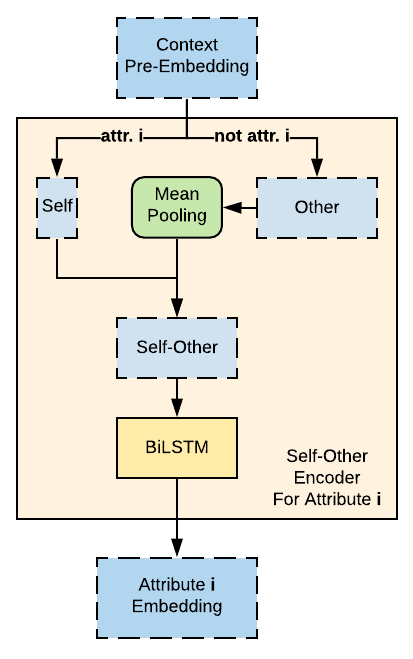
\includegraphics[height=12cm, width=.48\textwidth, keepaspectratio]{Figures/Ch2/boa_self_other_encoder.png}  }
\subcaptionbox{BoA encoder architecture.\label{fig:boa-encoder}}{
    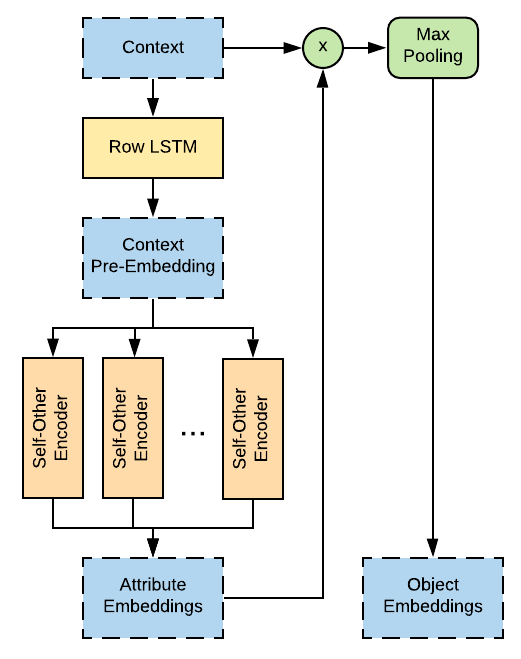
\includegraphics[height=12cm, width=.48\textwidth, keepaspectratio]{Figures/Ch2/boa_encoder.png}  }
\subcaptionbox{BoA decoder architecture.\label{fig:boa-decoder}}{
    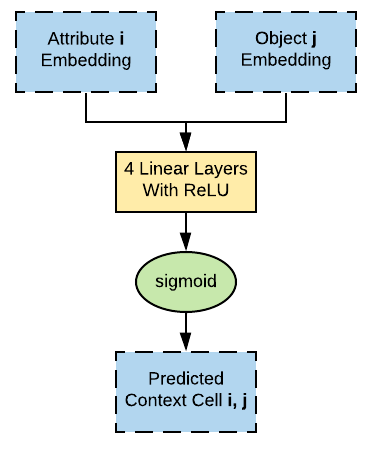
\includegraphics[height=12cm, width=.48\textwidth, keepaspectratio]{Figures/Ch2/boa_decoder.png}  }
\caption{Schematic representation of the BoA architecture. Blue blocks correspond to tensors, the orange to neural components and green blocks to non-neural computations. Arrows joining blocks represent concatenation of tensors.} \label{fig:boa-architecture}
\end{figure}

\textit{Bag of Attributes} (BoA) takes a formal context as input and produces embeddings for its attributes.
Then, object embeddings are computed using the embeddings of the attributes and the formal context.
BoA has four main components: a pre-embedding generator, an attribute encoder called \textit{self-other encoder} to compute the attribute embedding, an object encoder, and a decoder.
The order of the attributes in the FC does not matter for FCA, because intents are unordered sets of attributes.
Therefore, in BoA, the order of the attributes is ignored by design.
BoA considers the attributes as an unordered set to produce the object and attribute embeddings.
The name is an homage to \textit{Bag of Words} (BoW)~\cite{word2vec:2013:mikolov}, which consider sentences as unordered bags of words.

To capture the absence of order between the attributes, they are processed in a similar manner.
Each attribute is compared to all the other attributes, for each object of the FC.
In practice, the column of an attribute (\emph{self}) is compared to an unordered composition (average-pooling) of all the other attributes (\emph{other}).
\emph{Self} and \emph{other} are then concatenated and processed by a BLSTM, with the object dimension as the sequence dimension.
The last hidden state of the BLSTM is processed with a feed-forward layer into an embedding that represents the attribute.
The structure of the attribute encoder is presented in \cref{fig:self-other}.
A $\mu$ and a $\sigma$ vector are produced for each attribute because BoA is trained as a VAE, and the actual embeddings are samples from the normal distributions defined by $\mu$ and $\sigma$.
Finally, the object embeddings are computed by applying max-pooling on the embeddings of the attributes present in the object's intent.
The structure of the encoder is schematized in \cref{fig:boa-encoder}.

%\subsubsection{Pre-Embedding}
This encoder architecture successfully ignores the order of the attributes.
However, we are not able to differentiate between the attributes anymore either, which is a problem to model FCA.
Indeed, we still need to differentiate the attributes to know which ones belong in which intent, even if the order of the attribute does not matter.
Using unordered composition directly on the FC will prevent the model from differentiating, \eg, when an attribute $a_1$ is present and $a_2$ is not from when $a_2$ is present and not $a_1$:
the average of the list $(0, 1)$ is $0.5$, the same as the average of the list $(1, 0)$.
The same kind of problem arises with standard embedding methods using a learned vector to represent each possible value.
In our previous example, if we replace in $C$ every $1$ with the same embedding $emb_1$ and every $0$ by $emb_0$, the model is still unable to determine which one between $a_1$ and $a_2$ is present.
To avoid this issue, we apply an LSTM on each row of $C$ before the \textit{self-other encoder}.
This LSTM can produce different embeddings for each attribute despite the same input, so it allows the model to identify the attributes when the unordered composition is applied.
Indeed, RNNs produce different outputs from the same input if their hidden state is different.

The decoder is an MLP predicting if an object has an attribute or not ($1$ or $0$, respectively).
Its input is the concatenation of the object and the attribute embeddings.
A sigmoid function applied to the output ensures it is in $[0,1]$.
It is schematized in \cref{fig:boa-decoder}.


\subsection{Training Objective}\label{sec:boa-metric}
% We train our BoA model using four objectives.
% %
% The first two are the KL divergence and the reconstruction loss.
% In our case we predict between two classes ($1$ and $0$), so we use the \textit{binary cross entropy} loss for reconstruction.
% The KL divergence is applied on the attribute embeddings exclusively as the sampling happens before the computation of the object embeddings.
We train BoA using KL divergence on the attribute embeddings exclusively because the sampling happens before the computation of the object embeddings.
We use the BCE loss for reconstruction because the model predicts between two classes ($1$ and $0$).
To improve the quality of the embeddings, we use metric learning the \textit{co-intent similarity} (defined in the next paragraph) and the number of concepts~\cite{formal:1999:bernhard}, with \textit{mean square error} (MSE) as the loss function.
We use MLPs to predict the co-intent similarity and number of concepts.
The training setup is schematized in \cref{fig:boa-training}.

\begin{figure}
\centering
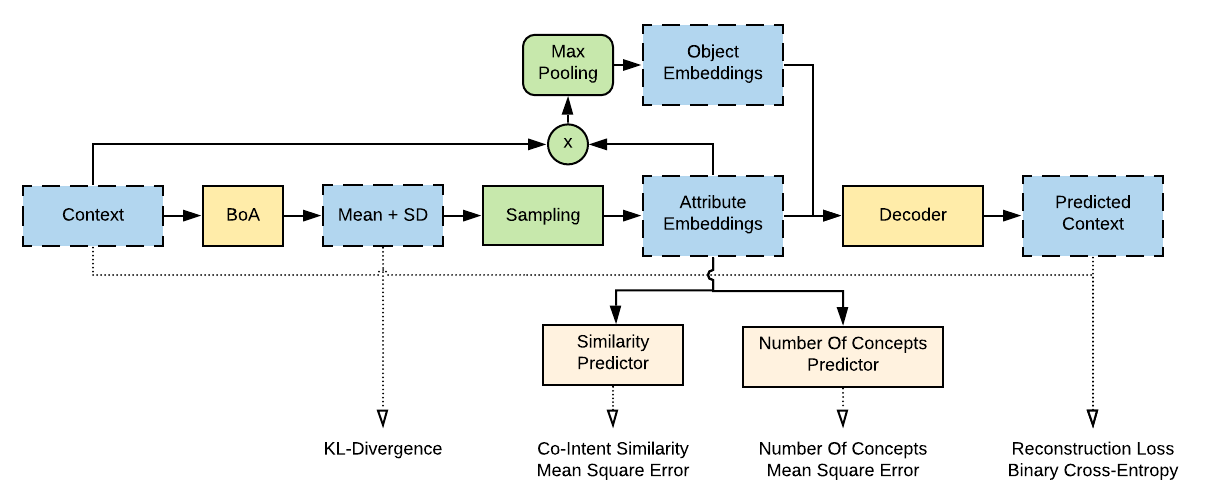
\includegraphics[height=12cm, width=\textwidth, keepaspectratio]{Figures/Ch2/training_flat.png}
\caption{Schematic representation of the BoA architecture training process.} \label{fig:boa-training}
\end{figure}

On the one hand, we need both ``equal'' and ``different'' attributes to use metric learning losses on attribute embeddings.
Nonetheless, even if we consider equivalent attributes (\textit{i.e.} with the same extent) as ``equal'', they are usually rare within a given context.
We define co-intent similarity to compare attributes and avoid this issue.
Given two attributes $a_1$ and $a_2$ we define their \emph{pairwise co-intent similarity} as:
\begin{equation}
\text{co-intent}(a_1, a_2) = 
%
\left\{
    \begin{array}{l}
        1 \text{~~~ if } |\{i\in I| a_1 \in i\}| + |\{i\in I| a_2 \in i\}| = 0 \\\\
        \dfrac{2 \times |\{i\in I| a_1 \in i, a_2 \in i\}|}{|\{i\in I| a_1 \in i\}| + |\{i\in I| a_2 \in i\}|} \text{ otherwise.}
    \end{array}
\right.
\label{equ:co-intent}
\end{equation}
In other words, it is the ratio of intents containing both attributes over the intents containing $a_1$ or $a_2$\footnote{Observe that this is essentially the Jaccard index on the set of intents.}.
In cases where no intent contains the attributes (both attributes are empty or padding columns), the similarity is set to $1$.
Co-intent similarity ranges from $0$, for attributes never appearing in the same intents, to $1$, for attributes always appearing together or for identical attributes.
To predict the co-intent similarity between two attributes $a_1$ and $a_2$, the input of the MLP predictor is the concatenated embeddings of $a_1$ and $a_2$, and a sigmoid output function is added to ensure the predicted similarity is in $[0,1]$.

On the other hand, predicting the number of concepts from the context without actually computing the intents, helps when generating the set of concepts using neural models.
Indeed, knowing how many elements to generate beforehand facilitates the generation process.
Note that counting the number of concepts of a context is \#P-complete (and so, is a ``hard'' task to achieve)~\cite{lattice-size:2001:kuznetsov}.
%\todo{Alain: As a remark, counting the number of concepts of a context is \#P-complete (and so, is a "hard" task to achieve)}
We apply a max-pooling over the attribute embeddings before predicting the number of concepts with the MLP predictor, which corresponds to a \textit{deep averaging network} (DAN)~\cite{dan:2015:iyyer}.



\section{Training\label{sec:boa-training}}
In this section, we explain how we train BoA.
We describe the training process in \cref{sec:boa-training-process} and the randomly generated dataset in \cref{sec:boa-training-data}. In \cref{sec:augment}, we define a data augmentation pipeline used to improve the generalization capacity of BoA and compensate for some of the biases of the random generation. Finally, we explain in \cref{sec:kl-problem} a problem we encountered with the variational aspect of BoA.

\subsection{Training Process}\label{sec:boa-training-process}
We train BoA in two phases of 5000 epochs each.
In the first phase, we apply the reconstruction loss and the KL divergence only.
Then, we gradually introduce the prediction of the co-intent similarity and the number of concepts.
%
When using metric learning with multiple distances, a common approach is to split the embedding space and to learn one distance per sub-part of the embedding space~\cite{deep-metric-multispeaker:2020:kulkarni}.
We apply the same principle and use 50\% of the embedding space to predict the co-intent similarity and 25\% for the number of concepts.
%
The exact embedding dimension of BoA is 128, with a pre-embedding size of 64.
The LSTM and the BLSTM have two layers each.
The decoder MLP has four layers, and the MLPs used for distance prediction both have two layers.
We use a ReLU activation function between all the layers of the model.

\subsection{Training Dataset}\label{sec:boa-training-data}
The dataset used for training BoA is composed of 6000 randomly generated formal contexts and the corresponding lattices split into training and validation.
We generate a training set of 5000 contexts and a test set of 1000 samples using the generation principle described in \cref{sec:data-generation}.
For the training phase, a development set of 10\% of the training set is randomly sampled from the training set. 
For each set, we generate different sizes of contexts, 20\% of each: $5 \times 5$, $10 \times 10$, $10 \times 20$, $20 \times 10$, and $20 \times 20$ contexts ($|O|\times|A|$).
We report statistics of the generated datasets in \cref{tab:rand-dataset}.

{%\smaller
\begin{table}[t]
\centering
\begin{tabularx}{\textwidth}{rr>{\raggedleft\arraybackslash}X>{\raggedleft\arraybackslash}X>{\raggedleft\arraybackslash}X>{\raggedleft\arraybackslash}X}
\toprule
 & Dataset\hspace{-0.5em} & \# Object & \# Attribute & \# Concept & Density of $C$ \\
\midrule
\multirow{2}{*}{Mean $\pm$~std.\hspace{-1em}}
& Train\hspace{-0.5em} & $12.83 \pm 6.11$ & $12.98 \pm 6.03$ & $77.93 \pm 78.39$ & $0.329 \pm 0.057$ \\
& Test\hspace{-0.5em}  & $12.83 \pm 6.13$ & $12.97 \pm 6.04$ & $78.12 \pm 77.27$ & $0.332 \pm 0.057$ \\
\midrule
\multirow{2}{*}{Range\hspace{-1em}}
& Train\hspace{-0.5em} & 1 to 20 & 2 to 20 & 1 to 401 & 0 to 0.56 \\
& Test\hspace{-0.5em}  & 2 to 20 & 3 to 20 & 2 to 401 & 0 to 0.49 \\
\bottomrule
\end{tabularx}
\caption{Descriptive statistics on the dataset of randomly generated contexts.}\label{tab:rand-dataset}
\end{table}
}

\subsection{Data Augmentation}\label{sec:augment}
We rely on plain random generation for the formal contexts, and not on more involved generation processes as discussed in~\cite{random-closure:2011:ganter,random-context-dirichlet:2019:felde}, so the random data is biased.
We introduce a simple way to compensate for some of those biases while improving the generalization capability of the model using \textit{data augmentation}.
In deep learning and machine learning in general, data augmentation is the process of artificially augmenting the amount of training data, typically by modifying existing training samples.
We implement the following data augmentation pipeline: \textit{(i)} duplicating of objects and attributes, \textit{(ii)} inverting (dropping) the value of entries, and \textit{(iii)} shuffling objects and attributes.
With this process, we simulate identical (duplication) and nearly identical (duplication + drop) objects or attributes that appear in real-world datasets.

Objects and attributes have a probability $p$ of being duplicated.
If duplicated, they have the same probability $p$ of being duplicated again.
From this definition, the number of copies of an object (or attribute) follows a geometric law with a probability of success $p$.
Consequently, the exact number of objects and attributes seen during training does not match the ones reported in \cref{tab:rand-dataset}.
Nonetheless, the duplication follows a geometric law so we can estimate the number amount of objects and attributes seen as $number/(1 - p)$.
Inverting some randomly selected values in the formal context is our adaptation of dropout, a common technique in deep learning.
The shuffling after duplication avoids the model's reliance on the order of the objects and the attributes.
We set the duplication probability to $p=0.1$ and the drop probability to $0.01$.
In this setting, the estimated average object and attribute numbers are respectively $14.25$ and $14.42$, for both the training and development sets.

When co-intent similarity is used, duplication and shuffling are reproduced on the intents.
However, drops in a formal context alter the corresponding lattice, so they are not applied when using the intents to compute co-intent similarity.
This precaution avoids making the model insensitive to small variations in the input.


\subsection{Issues With KL Divergence}\label{sec:kl-problem}
When adding the KL divergence to the prototype of BoA (initially a simple auto-encoder) the performance of the model was greatly impaired.
The analysis of the predictions revealed the model was going for ``low hanging fruits'' and ignored the embeddings themselves, as described in~\cite{annealing-kl:2015:bowman}.
To solve this issue we apply \textit{annealing}~\cite{annealing-kl:2015:bowman} and multiply the KL divergence by a lambda that we set to $10^{-3}$.
This reduces the impact of the KL divergence on the training and allows the model to learn some features before the KL divergence comes into effect.
However, it reduces the benefits we get from using a VAE.%\todo{Replace with "It reduces the benefits we get from using a VAE though."}



\section{Experiments}\label{sec:boa-expe}
In \cref{sec:boa-reconstruction} and \cref{sec:boa-metric-perf}, we explore the limits of BoA \textit{w.r.t.} input data.
In \cref{sec:boa-real-world-expe}, we reproduce the experiments from~\cite{fca2vec:2019:durrschnabel} on real-world data.
%In this section we explore the limits of our model with regards to the input data.
%We first examine the scalability of the approach, then we evaluate the sensitivity of the approach to perturbation of the data.
All the experiments described in \cref{sec:boa-reconstruction} and \cref{sec:boa-metric-perf} are performed on randomly generated data to control the of the evaluation process.
%(in terms of performance)

    
\subsection{Reconstruction Performance}\label{sec:boa-reconstruction}
To assess the reconstruction performance of the BoA auto-encoder, we use the \textit{area under the receiver operating characteristic curve} (AUC ROC).
It allows us to determine whether the BoA has a good predictive capacity and, similarly to the F1 measure, AUC ROC gives a general account of performance. %, as the receiver operating characteristics curve depends on precision and recall.
%AUC ROC goes from 0 to 1, with results close to $0.5$ corresponding to poor predictive performance and those closer to $1$ correspond to better models.
To determine if the results are significantly different, we use Student t-test on means.
The results are presented in \cref{fig:limits}.

\begin{figure}
\centering
\subcaptionbox{Impact of the density, from 0.1 to 0.9, 100 samples per density.\label{fig:limits_density}}
    {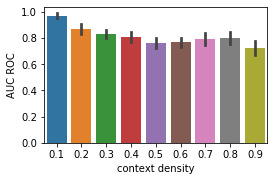
\includegraphics[width=.48\textwidth, height=4cm, keepaspectratio]{Figures/Ch2/limits_densities.png}  }
\subcaptionbox{Impact of the size, from 5 to 500 objects and attributes, 20 samples per size.\label{fig:limits_size}}
    {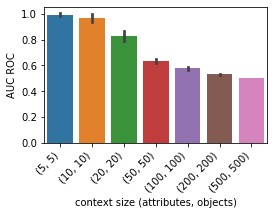
\includegraphics[width=.48\textwidth, height=4cm, keepaspectratio]{Figures/Ch2/limits_size.png}  }
\subcaptionbox{Impact of the concept number, for 200 sample with 20 objects and attributes. The blue line is the general tendency when rounding the concept number to 50.\label{fig:limits_concepts}}
    {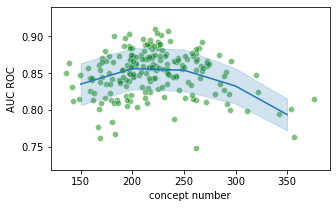
\includegraphics[width=.48\textwidth, height=4cm, keepaspectratio]{Figures/Ch2/limits_concepts.png}  }
\caption{Reconstruction performance on random contexts. The error bars and the shaded area correspond to the standard deviation.}\label{fig:limits}
\end{figure}

We first evaluate the impact of the density on the reconstruction by comparing the performance on random contexts with densities from 0.1 to 0.9.
% We first evaluate the impact of the density on the reconstruction AUC ROC.
% We compare the performance on random contexts with densities from 0.1 to 0.9, with a fixed size of 20 objects and 20 attributes.
We use 100 samples per density with a fixed size of 20 objects and attributes.
Student's t-test shows significant differences between the performance with the various densities: all the p-values are under 0.01 except between 0.4 and 0.8 (0.24), 0.5 and 0.6 (0.39), and 0.7 and 0.8 (0.19).
However, the model performance stays overall stable across the densities, while slightly better with smaller densities.
We suspect this tendency is due to the composition process of the object embeddings: the higher the density, the more attributes are present for an object, so more attribute embeddings are involved in the composition of the object embeddings, making it more complex to decode.

We also examine the effect of the size on the AUC ROC.
Square random contexts ($|O|=|A|$) of sizes in $\{5,10,20,50,100,200,500\}$ and a fixed density of 0.3 are used for this experiment,
with 20 samples per size.
The model performs very well for seen data sizes with a slight drop to $0.83$ for $20$ objects and attributes.
As expected, the performance drops when manipulating larger contexts. %When manipulating larger contexts the performance drops as we can expect.
For $50$ objects and attributes ($2.5$ times the maximum seen size), the AUC ROC is above $0.63$, but from $100$ objects and attributes onward, it drops under $0.6$.
Finally, with 500 objects and attributes (25 times the largest seen data size and 4 times the embedding size), the reconstruction AUC ROC falls to $0.50$ on average.
This is the limit of reconstruction performance with the current training process.

%\todo{Check this section with the FCA experts}
Finally, we examine the impact of the number of concepts on the performance of the model.
We use contexts of fixed size (20 objects and attributes) from the test set, totaling 200 contexts.
We consider the concept number as an indicator of the variety of attributes and objects in the context.
Indeed, if the concept number is high for a given size of context, we can expect the context to be close to the clarified context (context with no equivalent objects or attributes). This implies a lower amount of duplicate objects and attributes.
Besides, we can expect the model to have a harder time encoding and decoding irregular contexts than repetitive ones.
Consequently, the drop of the AUC ROC for higher concept numbers is not surprising.
However, we also observe a lower performance around $150$ concepts.
This second decrease requires further investigation.
%\todo{Find a plausible reason for the drop at $150$ concepts}
%Globally, the worst performance is still above 0.75, which is 

\subsection{Metric Learning Performance}\label{sec:boa-metric-perf}
We evaluate the performance of BoA for the co-intent similarity and number of concepts' prediction, by computing the attribute embeddings and applying the predictors trained together with the BoA model.
We use the 200 contexts of 20 objects and attributes from the test set.
The prediction results are reported in \cref{fig:metric}.

\begin{figure}
\centering
\subcaptionbox{Concept number.\label{fig:metric_concept}}{
    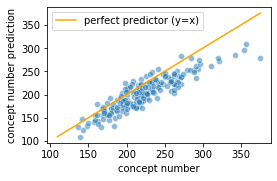
\includegraphics[height=3.5cm,width=.48\textwidth, keepaspectratio]{Figures/Ch2/metric_concept_number.png}  }
\subcaptionbox{Co-intent similarity.\label{fig:metric_cointent}}{
    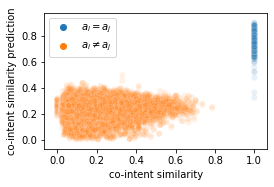
\includegraphics[height=3.5cm,width=.48\textwidth, keepaspectratio]{Figures/Ch2/metric_cointent.png}  }
\caption{Predicted metrics against the actual values, for the 200 samples with 20 objects and attributes from the test set.}\label{fig:metric}
\end{figure}

%\begin{figure}
%\centering
%\subcaptionbox{Number of concepts against size of the samples for square samples.}{\missingfigure[figcolor=white, figwidth=.48\textwidth]{Number of concepts against size of the samples?}}
%\subcaptionbox{Number of concepts upper bounds against size of the samples for non-square samples with 20 attributes.}{\missingfigure[figcolor=white, figwidth=.48\textwidth]{Number of concepts against size of the samples?}}
%\caption{Number of concepts and upper bounds against size of the FC, for a fixed density of $0.3$.}\label{fig:number-concepts}
%\end{figure}

The Pearson correlation coefficient is $0.9$ between the actual concept number and the prediction, indicating a strong correlation.
We can notice in \cref{fig:metric_concept} the tendency of the model to under-evaluate the concept number.
% and the p-value for testing non-correlation of $9.3 \times 10_{-74}$
We mention in \cref{sec:lattice-algo} a naive upper bound of the number of concept $2^{min(|O|,|A|)}$. In~\cite[p. 2]{lattice-size:2001:kuznetsov}, Kuznetsov mentions a more involved upper bound defined by Schütt:
$$3/2 \times 2^{\sqrt{|\mathbf{I}| + 1}} - 1$$
The density $d$ of the FC is such that $d = \frac{|\mathbf{I}|}{|O|\times|A|}$, so we can write $|\mathbf{I}| = d \times |O|\times|A|$.
%We show these two upper bounds compared to the actual number of concepts for the samples in our dataset and our predictions in \cref{fig:number-concepts}.
The predictions performed by our model are much smaller than the theoretical upper bounds of the number of concepts.
The prediction performance of the model is very helpful for our final goal, the generation of concepts, as mentioned in \cref{sec:boa-metric}.

When predicting the co-intent similarity, BoA manages to differentiate $a_i$ and $a_j$ when $a_i = a_j$.
However, the predictions in the other cases are not clear:
for similarities between $0$ and $0.8$, they seem randomly picked between $0$ and $0.4$.
%It appears the model has trouble learning the co-intent similarity.
The analysis of the training process reveals a small difference between the MSE of the first and the last training epochs: from $0.17$ to $0.05$.
Using MSE on values between 0 and 1 seems to cause the problem: an MSE of $0.05$ corresponds to an actual distance of around $0.22$, so 10\% of the interval of definition of co-intent similarity.
We envision several solutions, like changing the loss to \textit{mean absolute error} (MAE) or normalizing the similarity.
% In particular, normalizing and choosing a more appropriate loss could significantly improve the performance.
% We can expect that any improvement to the metric learning process would increase the quality of the embeddings.

%-> normalisation (log, exp,...) [0;1] ~> [0;inf[
%Suggestion mean-variance norm










\subsection{Experiments on Real-World Datasets}\label{sec:boa-real-world-expe}

To evaluate the performance of BoA on real-world datasets, we reproduce the link prediction and attribute clustering of~\cite{fca2vec:2019:durrschnabel}.
%
We use the same ICFCA dataset as~\cite{fca2vec:2019:durrschnabel} for link prediction.
However, for attribute clustering, we use SPECT heart\footnote{\url{https://archive.ics.uci.edu/ml/datasets/SPECT+Heart}} as it is smaller than {wiki44k}, with dimensions closer to the training data: 68 objects and 23 attributes.
Additionally, SPECT heart is much denser than wiki44k with a density of $0.23$.
Descriptive statistics on SPECT heart are reported in \cref{tab:spect}.

\begin{table}
    \centering
    \begin{tabular}{lllll}
    \toprule
    Dataset & \# Objects & \# Attributes & Density & \# Concepts\\
    \midrule
    SPECT heart & 68 & 23 & 0.23 & 911 \\
    \bottomrule
    \end{tabular}
    \caption{Descriptive statistics on SPECT heart.}
    \label{tab:spect}
\end{table}

We train the CBoW and SG variants of FCA2VEC models using the same settings as in~\cite{fca2vec:2019:durrschnabel}, with 20 random iterations of each model and an embedding size of 3.
To obtain comparable results, we reduce the embeddings produced by BoA to 3 dimensions by applying two standard dimensionality reduction techniques:
\textit{principal component analysis} (PCA) and \textit{t-distributed stochastic neighbor embedding} (TSNE).
We use Student's t-test on means to determine if the results are significant.

We report the link prediction performance in \autoref{tab:object}.
The three BoA variants show a significantly different performance from o2v SG, with all the p-values lower than $0.005$.
%
We found that the classifier based on BoA, the one with the best F1 score, systematically answers positive.
%Our TSNE variant seem performs normally however.
Additionally, we fail to reproduce the performance of~\cite{fca2vec:2019:durrschnabel} (F1 score of $0.69$ for o2v CBoW, $0.66$ for o2v SG)
Finally, the ICFCA context is very sparse: it has a density of $0.003$ on the train and $0.005$ on the test set.
Due to this, the task may not be representative of the performance of the object embeddings on most datasets.
%
These results hint that the task needs to be adapted to get proper insights into the object embedding performance.
%
%
The attribute clustering performance is reported in \autoref{tab:attribute}.
In this experiment, we find that the CBoW variant performs significantly better than the SG (all t-test p-values under $0.0005$).
This is the opposite of the result found by~\cite{fca2vec:2019:durrschnabel} for attribute clustering.
However, this result may be due to using a different dataset.
Interestingly, the BoA PCA variant performs equally to the full BoA.
The performance of BoA (and BoA PCA) is significantly better than a2v CBoW for 2 and 5 clusters (p-values under $10^{-14}$).
For 10 clusters however, a2v CBoW performs significantly better (p-value under $0.001$).
%
%Our model show a relative improment of 6\% for 2 clusters and 57\% for 5 clusters.
The model improves the performance of a2v CBoW by 4\% for 2 clusters and 8\% for 5 clusters.




\begin{table}[t]
\caption{Performance on the link prediction task (mean~$\pm$~std.).}\label{tab:object}
\centering
\begin{tabular}{lrrr}
\toprule
Model &  Precision & Recall & F1 \\
\midrule
o2v-CBoW    &  $0.63 \pm 0.05$ & ~$0.46 \pm 0.05$ & ~$0.53 \pm 0.05$ \\
o2v-SG      &  $0.70 \pm 0.04$ & $0.49 \pm 0.03$ & $0.57 \pm 0.02$ \\
\midrule
BoA PCA 3d  &  $0.65$ & $0.42$ & $0.51$ \\
BoA TSNE 3d &  $0.58$ & $0.67$ & ${0.62}$ \\
BoA         &  $0.50$ & $1.00$ & ${0.67}$ \\
\bottomrule
\end{tabular}
\end{table}


\begin{table}[t]
\caption{Performance on the attribute clustering task with 2, 5 and 10 clusters (mean~$\pm$~std.).} %(mean~$\pm$~std.)
\label{tab:attribute}
\centering
\begin{tabular}{lrrr}
\toprule
Model              & k = 2 & k = 5 & k = 10 \\
\midrule
a2v-SG             & $0.35 \pm 0.13$ &  $0.11 \pm 0.03$ & $0.042 \pm 0.010$ \\
a2v-CBoW           & $0.66 \pm 0.00$ &  ~$0.14 \pm 0.02$ & ~${0.063 \pm 0.013}$ \\
\midrule
BoA TSNE 3d & $0.30$ & $0.29$ & $0.044$ \\
BoA PCA 3d  & ${0.70}$ & ${0.22}$ & $0.051$ \\
BoA         & ${0.70}$ & ${0.22}$ & $0.051$ \\
\bottomrule
\end{tabular}
\end{table}



\chapter{Second Approach: Intents Generation\label{ch:intents}}
BoA allows us to generate embeddings of attributes and objects, and to reconstruct the FC from those embeddings.
As we have a representation of objects, which can be seen as sets of attributes, we can use this same representation for intents, which are also sets of attributes.
The reconstruction performance of BoA should allow us to generate intent embeddings and to decode them.

%\todo[inline]{\large Grammarly up to here}

Based on those results and the results of our preliminary experiments described in \cref{sec:prelim}, we designed a 4 phase approach to build an intent generation model:
\begin{enumerate}
    \item train a BoA auto-encoder;
    \item train a simple model to predict an upper bound of the number of concepts from the attribute embeddings, based on the predictor learned with BoA;
    \item design a model to predict the intents and the cover and order relations, using LSTM and the attention mechanisms tested in the preliminary experiments;
    \item as we expect the previous model to produce imperfect results given the performance of the preliminary models, an additional can be designed to ``refine'' the results.
\end{enumerate}
Once the whole system is finished, a final fine-tuning of the whole system should be performed.
%
This approach allows us to split the task into simpler problems.
Each phase produces a layer of the final model, and allows to train and evaluate them independently.
Consequently, it is easier to determine the weak-points of the architecture and improve the architecture accordingly.
Additionally, the first phase is already solved and the second one should be trivial.
This second approach is closer to the naive concept generation algorithm than the graph-based approach, because we first generate the set of intents and then compute the order between them.

%We at least have a lower bound for the results of the \nth{3} phase: the results of the exploratory process.
We successfully implemented this approach, with the BoA model, a DAN upper bound predictor, and an attention-based LSTM lattice generator, respectively described in \cref{ch:boa}, \cref{sec:upper-bound}, and \cref{sec:intent-generation}.
However, due to time constraints, we focused on improving the results of phase 3 instead of designing and training the ``refiner'' of phase 4.
Such modification of the approach do not prevent us form providing results for the rest of the architecture, which is one of the advantages of our modular approach.
We describe our training process and the performance of our current model in \cref{sec:fcat-expe}.





\section{Pilot Experiments}\label{sec:prelim}
In this section, we explain our preliminary experiments which led to the design of our intent generation model.
The goal of the pilot experiments presented in this section is to determine if a specific architecture could benefit our task, so we consider simple variants of major architecture families which could fit our goal. Also, the architectures are not trained to their maximum, and even if the results are not conclusive, it does not mean that an architecture in itself has no potential. However it hints a lower potential improvement of the performance for our task.
We consider 3 families of architectures for the task, each requiring some preliminary assumption on the size of the data:
\begin{itemize}
    \item the VAE architecture requires to have a fixed input and output size, so all the dimensions ($|O|$, $|A|$, and $|I|$) must be defined when creating a model; it is presented in \cref{sec:prelim-vae};
    \item the CNN architecture only requires to have a fixed $|I|$; it is presented in \cref{sec:prelim-cnn};
    \item the LSTM architectures only require to have a fixed $|A|$; it is presented in \cref{sec:prelim-lstm}.
\end{itemize}
We explain those limitations in the following subsections.
In each case, a model will be able to handle smaller inputs and outputs, but nothing larger than the values given creating the model.


%The results presented here all follow the same structure: first row is the output of the model (the prediction), and second row is the expected output. each column correspond to a sample of the data (one context/lattice pair).

\subsection{Variational Auto-Encoder Architecture}\label{sec:prelim-vae}
The VAE architecture is structurally the simplest of all the tested architecture.
It takes as an input a flattened FC at once and the output is reshaped into an intent matrix.
The encoder and the decoder are two MLPs. A block diagram of the architecture is shown in \cref{fig:prelim-vae-block}.

Using MLPs directly forces the input and output to always have the same size.
In this setup, we need to define $|O|$, $|A|$, and $|I|$ when we create the model.
Typically, those should be the maximal values in dataset of $|O|$, $|A|$, and $|I|$.
Using padding will allow us to process samples with smaller dimensions, but the model will be unable to process larger samples without loosing information.

This architecture is very simple and performs well, as shown in \cref{fig:prelim-vae}.
Indeed, the VAE seems to produce the expected shape and spread of the attributes across the contexts: few attributes for the intents close to $\top$, and more and more attributes until we reach $\bot$.
However, the fixed input and output size is a major drawback of this approach.

\subsection{Convolutional Neural Network Architecture}\label{sec:prelim-cnn}
The CNN architecture offers flexibility in the size of the input and output.
However, the size of the output of a CNN is proportional to the size of its input (due to the convolution principle).
In our case, it would mean that the number of predicted concepts would be directly proportional to the number of objects, which seems quite strange especially since that the theoretical upper bounds (see \cref{sec:boa-metric}) make the number of concept an exponential of the size of the FC.
With a standard CNN, the relation between the number of input objects and the number of output intents would have to be defined when designing the architecture, which seems unreasonable due to the explosive nature of the number of potential concepts.
 
To avoid the issue described above, we use one output \textit{channels} of the CNN for each concept, leading to the architecture schematized in \cref{fig:prelim-cnn-block}.
Consequently, we do not have a relation between the number of objects and the number of concepts nor any constraint on the number of objects, even if we still require the maximum $|I|$.
Interestingly, there is a full ``view'' on the data dedicated to each concept because each channel serves as a parallel and independent ``view'' on the FC.
The tested CNN requires a lot of parameters to compensate for removing the constraint on the object number. This large amount of parameters and its internal structure gives it a greater learning capability than the VAE. 

As shown in \cref{fig:prelim-cnn}, the shape of the output is close to the expected one and the spread of the attributes matches the expected output, similarly to the results of the VAE.
The results of the CNN look a little more random than the ones of the VAE, even if the ``texture'' (the sharpness of the result) of the predictions by the CNN is closer tho the expected output than the one produced by the VAE.
This approach seem to perform comparably to VAE, but with only a constraint on $|I|$.

\begin{figure}
    \centering
    \subcaptionbox{VAE\label{fig:prelim-vae-block}}{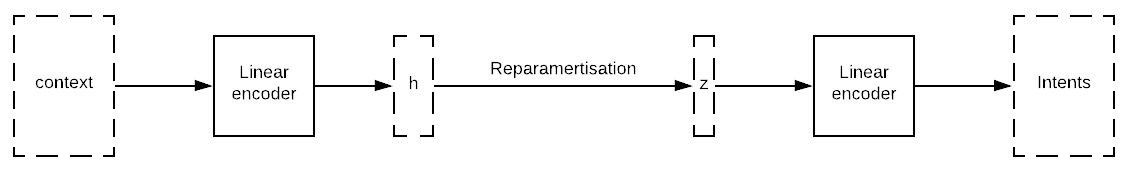
\includegraphics[width = .9\textwidth, height = 4cm, keepaspectratio]{Figures/Ch3/vae_block.png}}
    \subcaptionbox{CNN\label{fig:prelim-cnn-block}}{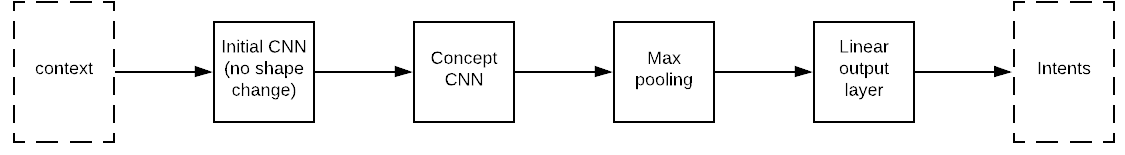
\includegraphics[width = .9\textwidth, height = 4cm, keepaspectratio]{Figures/Ch3/cnn_block.png}}
    \caption{Block diagrams of the VAE and CNN architectures.}
\end{figure}

\begin{figure}
    \centering
    \subcaptionbox{VAE\label{fig:prelim-vae}}{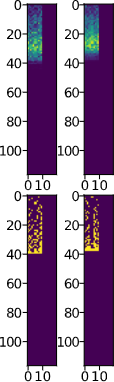
\includegraphics[width = .9\textwidth, height = 6cm, keepaspectratio]{Figures/Ch3/vae.png}}
    \subcaptionbox{CNN\label{fig:prelim-cnn}}{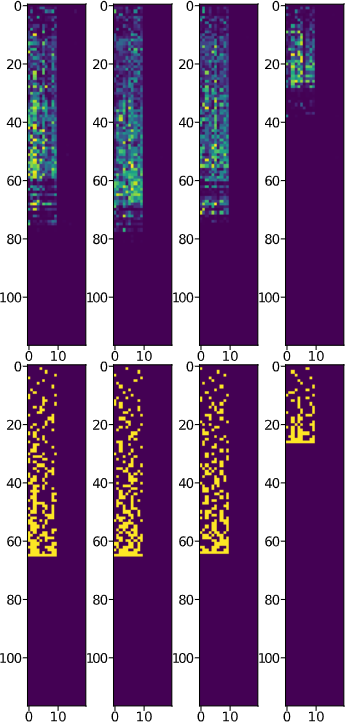
\includegraphics[width = .9\textwidth, height = 6cm, keepaspectratio]{Figures/Ch3/cnn.png}}
    \caption{Examples of results of the VAE and CNN architectures. In the images, a blue pixel corresponds to a $0$ and a yellow one to $1$. The first row correspond to the prediction by the model and the second row is the actual intent matrix. Each column correspond to a different sample in the same batch.}
\end{figure}

\subsection{Recurrent Neural Network Architecture and Attention Mechanisms} \label{sec:prelim-lstm}
\begin{figure}
    \centering
    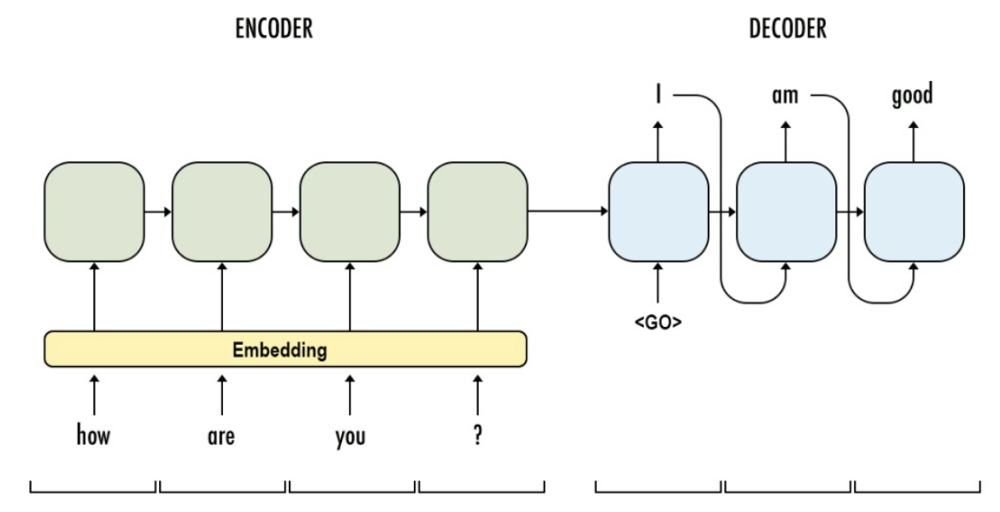
\includegraphics[width = .8\textwidth, height = .4\textwidth, keepaspectratio]{Figures/Ch3/seq2seq.png}
    \caption{Example of a sequence to sequence RNN, figure from~\cite{nlp:2018:aditya}.}
    \label{fig:seq2seq}
\end{figure}

We use LSTM as a sequence to sequence model (\textit{seq2seq}), a common way to use the RNN to produce an output which does not have the same size as the input, \eg, \cref{fig:seq2seq}. Indeed, in our case, the number of concepts is different from the number of objects.
We use the attribute dimension as the input and output size, and the object and concept dimension as the sequence dimension. Due to this, the model is constrained the maximum $|A|$.
We experiments with a few variants of attention mechanisms:
\begin{itemize}
    \item \textit{soft-attention}, which compute a summary of all the inputs with respect to the current output, and use this summary to improve the current output;
    \item \textit{self-attention}, which compute a summary of the previous outputs with respect to the current output, and use this summary to improve the current output;
    \item a variant for our case of self-attention: \textit{link-attention}, which compute the similarity of the previous outputs with respect to the current output, and this similarity (between 0 and 1) serves as a link prediction; more precisely, the similarity between previous output $i$ and current output $j$ represent the probability to have a link between concept $i$ and concept $j$.
\end{itemize}
We use a simple version of attention, with $\cdot$ the dot product, $q$ the \textit{query} (the current LSTM output in our case), $s$ the sequence. We first compute the attention weight for a value $v\in s$ as $w_{q, v} = q \cdot v$, and apply a softmax on all the weights. Because after the softmax the sum of the weights is 1, the attention context $a_{q,s} = \sum_{v\in s}{w_{q, v}}$ also corresponds to the weighted average of the input sequence.
The global structure of the recurrent architecture is presented in \cref{fig:lstm_block}, with the three attention mechanisms in different colors.
Because we want to check whether using a specific attention mechanism improves the output, we test 5 variants of the architecture listed bellow, and compare the results along the arrows on \cref{fig:rnn_variants}.

\begin{figure}
    \centering
    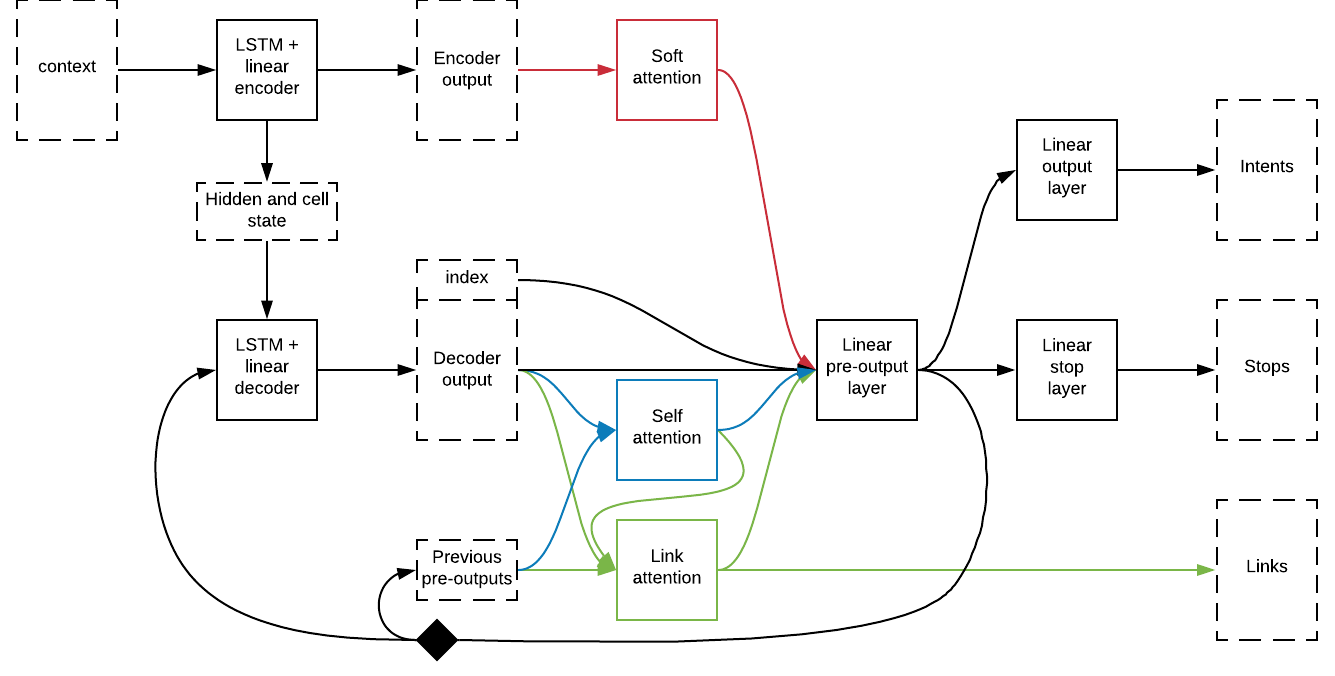
\includegraphics[width = .8\textwidth, height = .4\textwidth, keepaspectratio]{Figures/Ch3/lstm_block.png}
    \caption{Block diagram of the recurrent architectures.}
    \label{fig:lstm_block}
\end{figure}

The \textit{basic} model uses no attention, and takes the FC as a sequence of objects in input, and produces a sequence of intents in output.
Also, a second output is produced: the stop vector. It serves to determine when to stop generating intents during real-case usage.
In this specific implementation, the stop vector contains 1 if the corresponding row is a context intent, 0 if it is just padding.
%
The \textit{soft-attention} model extends the basic model with the soft-attention mechanism, which should improve the relevance of the output \textit{w.r.t.} the input because the model has a better access to the input information.
%
The \textit{self-attention} model extends the basic model with self-attention, which should improve the internal coherence of the output, as the model has a better access to the previously generated intents. We should obtain, \eg, a gradient from the empty set to the full set of attributes and a better prediction of the stop vector.
%
The two attention mechanisms are used in the \textit{bi-attention} model, so we can expect this model to bring the improvements of the self- and soft- attention together.
%
Finally, the \textit{tri-attention} model extends the bi-attention model with a link-attention as predicted above.
It generates an additional output: the links between the concepts, in other words the adjacency between the concepts. In our case we predict $\leq$, as we expect it to be easier to learn then $\prec$. Indeed, for $\leq$, a generic subset relation is enough, while for $\prec$ an additional step is required.

\begin{figure}
    \centering
    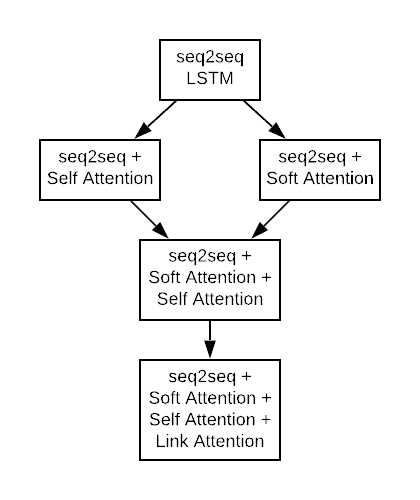
\includegraphics[width = .8\textwidth, height = .4\textwidth, keepaspectratio]{Figures/Ch3/rnn_attention.png}
    \caption{Hierarchy of the tested recurrent architecture variants}
    \label{fig:rnn_variants}
\end{figure}

The basic model performs quite bad (see \cref{fig:rnn}), which is to be expected given the complexity of the data and the relative simplicity of the model. All the produced intents look similar, and are most likely a sort of average of all the intents in the training set, and the stop vector is not at all predicted. Not much impact of the input can be seen, which is to be expected: it is too ``far'' from the output for a simple LSTM to handle. 
%
The soft-attention improves the model in a noticeable, and expected, manner: the output now has the same number of attributes as the input (see \cref{fig:soft}).
%
The self-attention also fulfills our expectations: the output has a nicer gradient (compared to the basic model) and the stop vector begins to be predicted correctly.
An unexpected improvement is that the output now also has the same number of attributes as the input.
In \cref{fig:self} display those improvement, and one can also notice an interesting ``bar'' around the end of the prediction, which seem to correspond to $\bot$, hinting a large potential improvement of the stop prediction in case of further training.
%
The bi-attention produces the expected results too: the output has the correct number of attributes, a the stop vector is closer to the expected one, and the length of the output matches quite well the expected one (as we can see on \cref{fig:bi}, with sample 2 being predicted slightly longer than sample 3, which matches the expected output).

However, the tri-attention produces both expected and unexpected effects. 
As expected, the links in  \cref{fig:tri2} look close to the expected output which hints that link attention is beneficial and can be used to predict the relations between concepts.
%
A first noteworthy point is that the performance of the model varies from good (see \cref{fig:tri2}) to bad, depending on the random initialization. We suppose that training all 3 outputs (intents, stops and links) at the same time from scratch, is too much for the model, and that training one aspect alone before introducing the others could avoid this type of issue. The negative impact of those training issues on the performance cannot be neglected.
%
The second interesting point is that the stops in \cref{fig:tri2} are close to the expected output, and the intents and links are clearly impacted by the stops.
%
Finally, we don't have too much of a degradation of the performance from the bi-attention model despite the training difficulties, even if the number of attributes is less well-predicted. 

\begin{figure}
    \centering
    \subcaptionbox{Extract of a result with the the recurrent model.
    \label{fig:rnn}}{
    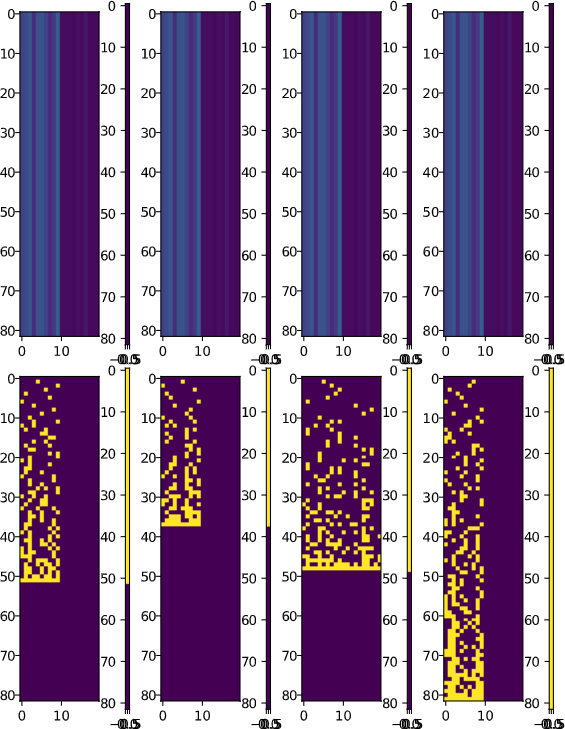
\includegraphics[width = .8\textwidth, height = .35\textwidth, keepaspectratio]{Figures/Ch3/rnn.png}}\hspace{2em}
    \subcaptionbox{Extract of a result with the soft-attention model.
    \label{fig:soft}}{
    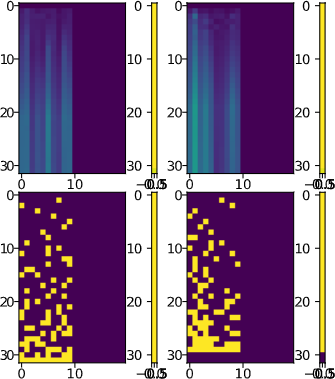
\includegraphics[width = .8\textwidth, height = .35\textwidth, keepaspectratio]{Figures/Ch3/soft.png}}\hspace{2em}
    \subcaptionbox{Extract of a result with the self-attention model.
    \label{fig:self}}{
    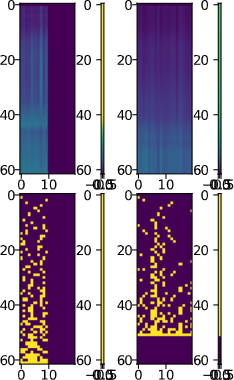
\includegraphics[width = .8\textwidth, height = .35\textwidth, keepaspectratio]{Figures/Ch3/self.png}}
    
    \subcaptionbox{Extract of a result with the bi-attention model.
    \label{fig:bi}}{
    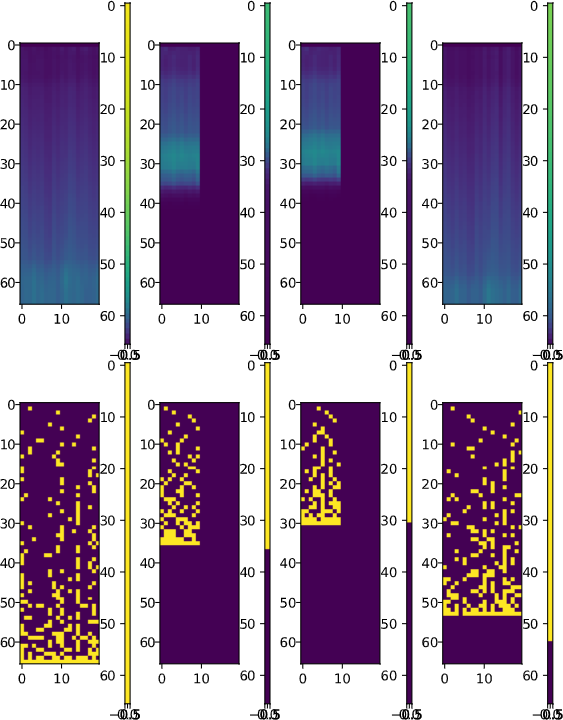
\includegraphics[width = .8\textwidth, height = .35\textwidth, keepaspectratio]{Figures/Ch3/bi.png}}\hspace{2em}
    \subcaptionbox{Extract of a result with the \nth{2} iteration of the tri-attention model.
    \label{fig:tri2}}{
    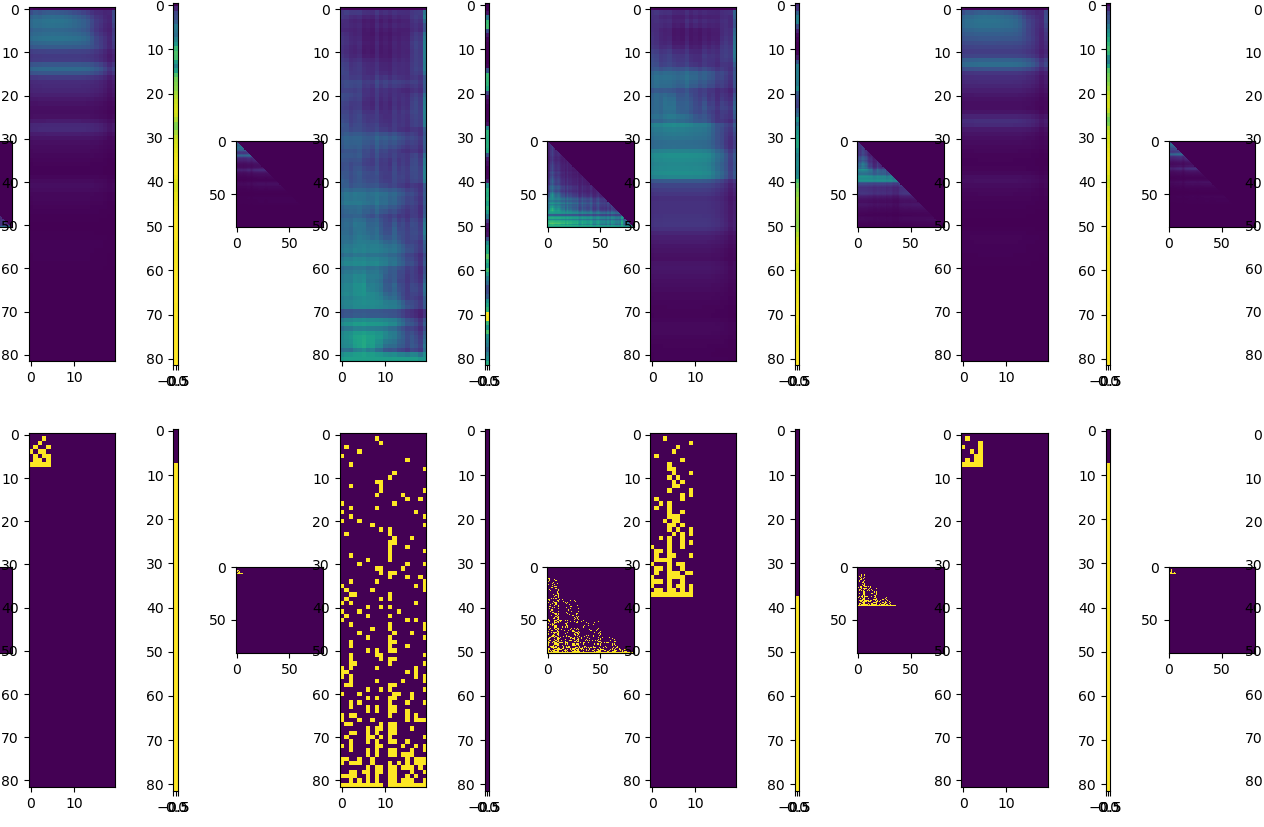
\includegraphics[width = .8\textwidth, height = .35\textwidth, keepaspectratio]{Figures/Ch3/tri2.png}}\hspace{2em}
    %\subcaptionbox{Extract of a result with the \nth{3} iteration of the tri-attention model.
    %\label{fig:tri3}}{
    %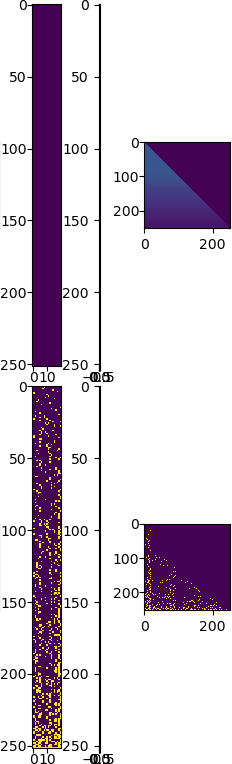
\includegraphics[width = .8\textwidth, height = .35\textwidth, keepaspectratio]{Figures/Ch3/tri3.png}}
    \caption{Extract of results on the test set with the various variants of the LSTM model. In the images, a blue pixel corresponds to a $0$ and a yellow one to $1$. The first row correspond to the prediction by the model and the second row is the actual intent matrix. Each column correspond to a different sample in the same batch.}
\end{figure}

\subsection{Conclusions on the Tested Architectures}
In conclusion, the VAE has heavy constraints on the dimension of the data which are not compatible with our goal, even if the architecture is simple, the training fast and the results among the best of all the studied architectures.
The CNN is not very accurate. However, it manages to capture the shape of the expected data, and thus could be used to reffine the more ``blurry'' output of the recurrent models.

The LSTM architectures are flexible enough for practical use, and the various attention mechanisms improve the performance by a notable margin in addition to providing with tools for the interpretability of the results of the model.
Also, the link attention process seem to have potential, but the way it interacts with the rest of the output and the training process both have to be revised.
%
Note that the LSTM architectures are applied directly on the FC.
Applying this approach on the embeddings generated by BoA should allow us to improve the performance.
More importantly, by replacing the attribute dimension by the embedding dimension, the resulting architecture can be applied in virtually any size of FC.

\section{Concept Number Upper Bound Prediction}\label{sec:upper-bound}
In sequence generation, there are two approaches on how to generate the correct number of elements.
The first option is to interrupt the generation based on a value generated at each step by the model, \eg, a stop value equal to 1 when generating the last element.
The alternative is to determine the number of elements beforehand and generate exactly this number of elements.
To generate the correct number of intents, we decided to use the second option, given the performance of the concept number predictor learned with BoA. Indeed, the number of intents is equal to the number of concepts in the lattice.

In our case, we have a margin of error in the predicted number of concepts $\hat{|I|}$.
Indeed, the generative model (phase 3 of the approach) will be able to compensate by filling the excess space with empty intents if $\hat{|I|}$ is higher than the actual number of concepts.
However, if $\hat{|I|}$ is too low, the generative model will not have enough space to generate the intents.
In short, we need an upper bound of the number of concept rather than the number of concept itself.
The additional freedom makes it easier to design a model fitting our needs.

We could use a theoretical upper bound, but those are rather large and increase exponentially with the size of the data (see \cref{sec:boa-metric-perf}).
Instead, we train a MLP to predict an upper bound of the concept number, from the prediction of the model learned with BoA and an average-pooling of the attribute embeddings. We train this model using an adapted MSE described in \cref{equ:upper-bound-loss}, with $p$ the target and $q$ the predicted number of concepts.
This new loss function first shifts the prediction target 10\% higher than the actual concept number, and penalizes predictions under the target by multiplying the squared error by 100 (an arbitrary number which provided good results).

We show in \cref{fig:concept-upper-bound} the upper bounds predicted on the validation set.
Of the 1000 samples tested, less than 1.2\% of the predictions are under the actual concept number.
The remaining prediction are close to the actual numbers, in average around 125\% of the true concept number.

\begin{figure}
    \centering
    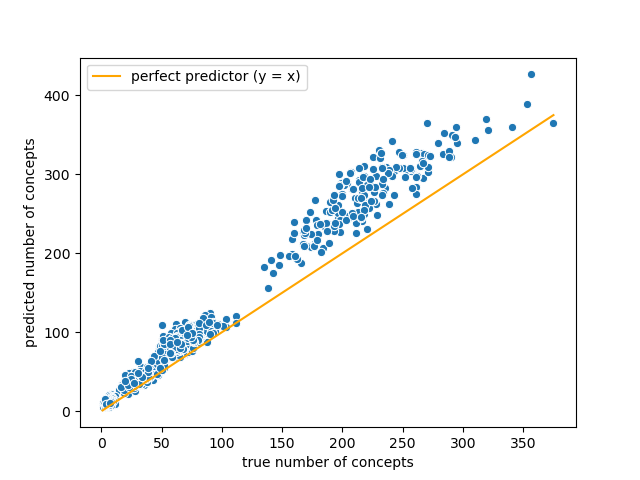
\includegraphics[keepaspectratio, width=.9\textwidth]{Figures/Ch3/concept_upper_bound.png}
    \caption{Upper bounds predicted by the model on all the samples of the evaluation set.}
    \label{fig:concept-upper-bound}
\end{figure}

\begin{equation}
    \begin{split}
        ShiftedError(p, q) &= q - (p \times 1.1)\\
        UpperBoundError(p, q) &= ShiftedError(p, q)^2 \;\text{~~if } ShiftedError(p, q) > 0\\
        &= 100 \times ShiftedError(p, q)^2 \;\text{~~otherwise}
        \label{equ:upper-bound-loss}
    \end{split}
\end{equation}
\section{Intents, Cover and Order Relation Generation}\label{sec:intent-generation}

Our initial design for the intent prediction was split into 3 modules:
\begin{enumerate}
    \item the first module would create a skeleton for the intents, from the concept number upper bound and the attribute embeddings;
    \item the second module would predict the intents, from the skeleton and the object and attribute embeddings;
    \item the last module would use the intents and the attribute embeddings to predict the links; this last module wouldn't share its gradient with the first two.
\end{enumerate}

Experimental results led us to simplify the model by merging the 3 modules into a simpler model described in \cref{fig:fcat}.
The resulting architecture relies on a DAN, an LSTM, and attention mechanisms described in the next paragraphs.
The DAN takes the attribute embeddings as input, and generates a single output per FC which is then used at every step of the generation process, as shown in \cref{fig:fcat}.
We expect it to learn general information about the FC similarly to how the number of concept prediction works.
In addition to the output of the DAN and the attention contexts, the LSTM is fed the number of concept upper bound and the index of the current intent.

\begin{figure}
    \centering
    \subcaptionbox{Concept generator at step $k$}{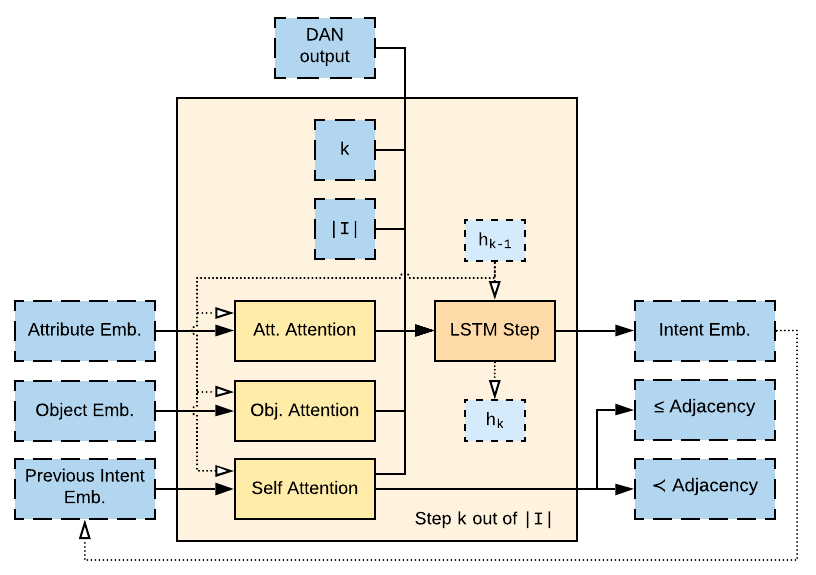
\includegraphics[keepaspectratio, height=5cm, width=.48\textwidth]{Figures/Ch3/fcat_cell.png}}
    \subcaptionbox{Full architecture}{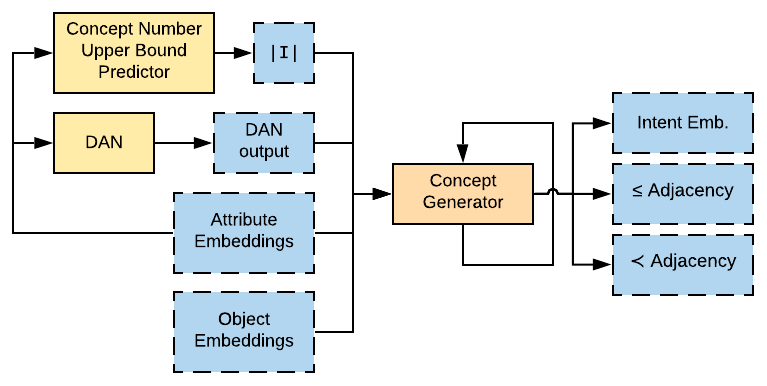
\includegraphics[keepaspectratio, height=5cm, width=.48\textwidth]{Figures/Ch3/fcat_full.png}}
    \caption{Schematic representation of the intent generation architecture. Blue blocks correspond to tensors and orange to neural components.}
    \label{fig:fcat}
\end{figure}

For intent generation we use a basic version of attention, equipped with multiple attention heads.
Attention heads can be seen as reading heads scanning the same sequence, but each head performing a different scan.
Our attention mechanism works by comparing a query $q$ with sequence $S$ of elements.
The query at step $k$ of the generation is obtained by flattening the hidden state generated at step $k-1$.

Let $\varphi$ be a feed-forward layer with input and output size $|s|$ for $s\in S$.
Let $\psi_i$ be a feed-forward layer associated with head $i$ with input size $|q|$ and output size $|s|$.
Finally, let $\cdot$ be the dot product.
The attention weight computed by head $i$ for element $s$ can be expressed as $weight_i(s,q) = \varphi(s) \cdot \psi_i(q)$.
A softmax is applied to all the weights of an head, which are then used to compute the attention summary $summary_i(S,q) = \sum_{s\in S} softmaxedWeight_i(s,q) \times \varphi(s)$.
We also use a sigmoid variant of our attention for which the weights are $weight_i(s,q) = sigmoid(\varphi(s) \cdot \psi_i(q))$.

In our model we use 3 attentions, each equipped with 4 heads, for a total of 12 attention heads:\begin{itemize}
    \item an \textit{object attention}, an attention applied on the set of object embeddings;
    \item an \textit{attribute attention}, an attention applied on the set of attribute embeddings;
    \item a \textit{self attention}, an attention applied on the previously generated intents.
\end{itemize}
Two of the self attention heads are of the sigmoid variant, and are used to predict the relations between the currently seen intent (or concept) and the attended intent (or concept). The sigmoid attention weight serve as a probability of there being an edge between the current concept and the previous one, \textit{à la} GraphRNN.
One of the heads is dedicated to $\leq$ and the other to $\prec$.

Compared to our preliminary experiments, the soft attention is split in two because there are two input sequences, and the link attention correspond to the two sigmoid attention heads of the self attention.



\section{Training and First Experiments}\label{sec:fcat-expe}
% training process
We use the training process schematized in \cref{fig:fcat-training} to train our intent generation model on the dataset used for BoA.
For details on the data, refer back to \cref{sec:boa-training-data}.
We train the intent model with BCE on the intent matrix and the cover and order relation.
We also use MSE between the generated intent embeddings and the expected intent embeddings, produced by applying the object embedding process of BoA on the intent matrix.
Using MSE on the expected intent embedding has proven, experimentally, to improve the performance and convergence speed compared to using only the BCE on the intent matrix.
We also confirmed that the intent prediction performance was not hindered by the BCE for the order and cover relations.
Finally, retraining the BoA decoder with the rest of the model converges faster but performs worse than training only the intent model.

\begin{figure}
\centering
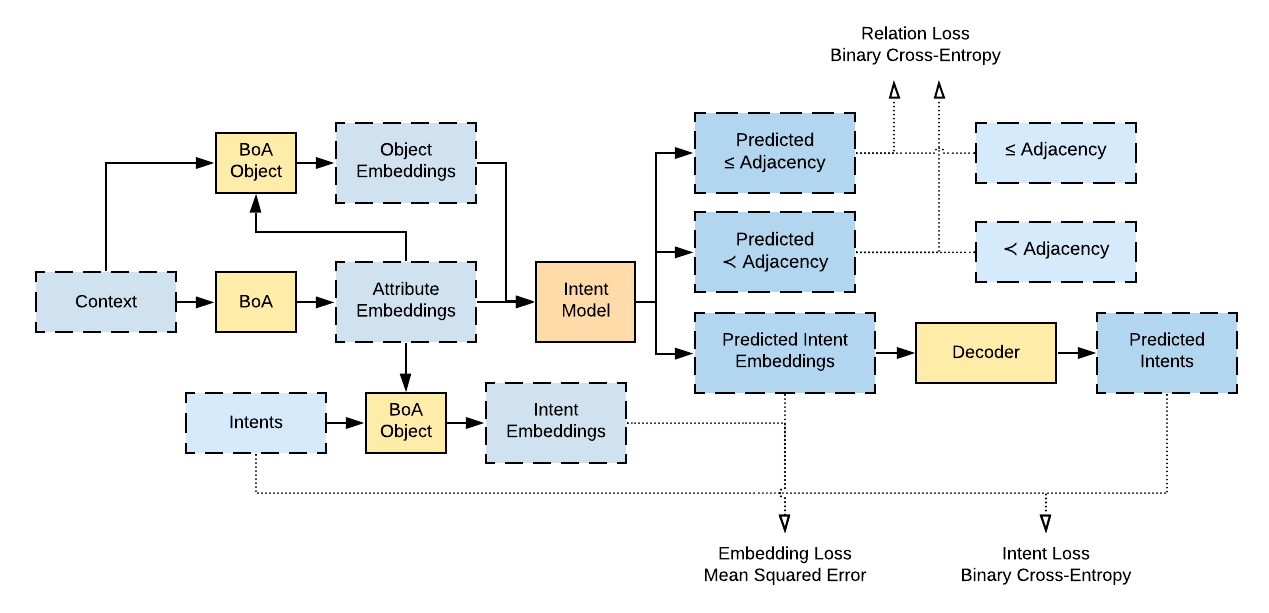
\includegraphics[height=12cm, width=\textwidth, keepaspectratio]{Figures/Ch3/fcat_training.png}
\caption{Schematic representation of the intent model training process.} \label{fig:fcat-training}
\end{figure}

We rely on two sets of measures to evaluate the performance of our model for intent generation.
First, we determine the predictive performance at the scale of each component of the intent matrix using AUC ROC.
%Then, we determine the best threshold using the ROC and apply it on the intent matrix.
Then, we apply a threshold of $0.5$ on the intent matrix.
We transform the resulting matrix into a set of predicted intents $\hat{I}$, so we remove all duplicate predicted intents.
After removing the duplicates from the set versions of the intents, we compute the intent precision as ${|\hat{I}\cap I|}/{|\hat{I}|}$ and the recall as ${|\hat{I}\cap I|}/{|I|}$. From the precision and recall we can compute the F1 score.
%
We also use the AUC ROC to measure the prediction performance on the relation prediction by the attention, for both $\leq$ and $\prec$.
We apply it on the adjacency vector of the relations, as described in \cref{sec:enc-adjacency}.

We report the performance on our evaluation set in \cref{tab:fcat-perf}, and show the prediction result for a few samples of the training set in \cref{fig:fcat-perf}.
The model presented was trained for 12h which corresponds to 50 epochs.
The AUC ROC for the two relations $\leq$ and $\prec$ is close to $0.85$ which is not perfect but not bad either.
However, the AUC ROC on the intent matrix is $0.72$, which is still above a random model but is not good enough for our application.
Indeed, the precision on the intents is under 25\% in average, and the recall and F1 are under 10\%.
The qualitative results displayed in \cref{fig:fcat-perf} are better than the ones obtained in the preliminary experiments.
It is interesting to note that for the first of the two samples, the first 50 predicted concepts look similar and are processed similarly by the attention generating the order relation, resulting in a slightly denser column between 0 and 50 in the adjacency of $\leq$ (\nth{6} column of the picture. This indicates that the intent and the relations are related within the model.


\begin{table}[t]
\centering
\begin{tabular}{rr}
\toprule
Measure & Mean $\pm$ std. \\
\midrule
Intent precision              & $ 0.217\pm 0.224 $ \\
Intent recall                 & $ 0.071\pm 0.092 $ \\
Intent F1                     & $ 0.046\pm 0.054 $ \\
%Intent miss rate              & $ 0.929\pm 0.092 $ \\
%Intent false discovery rate   & $ 0.783\pm 0.224 $ \\
\midrule
Intent matrix AUC ROC & $ 0.720\pm 0.062 $ \\
$\leq$ AUC ROC        & $ 0.852\pm 0.071 $ \\
$\prec$ AUC ROC       & $ 0.846\pm 0.072 $ \\
\bottomrule
\end{tabular}
\caption{Performance of the intent model on the evaluation set.}\label{tab:fcat-perf}
\end{table}

\begin{figure}
    \centering
    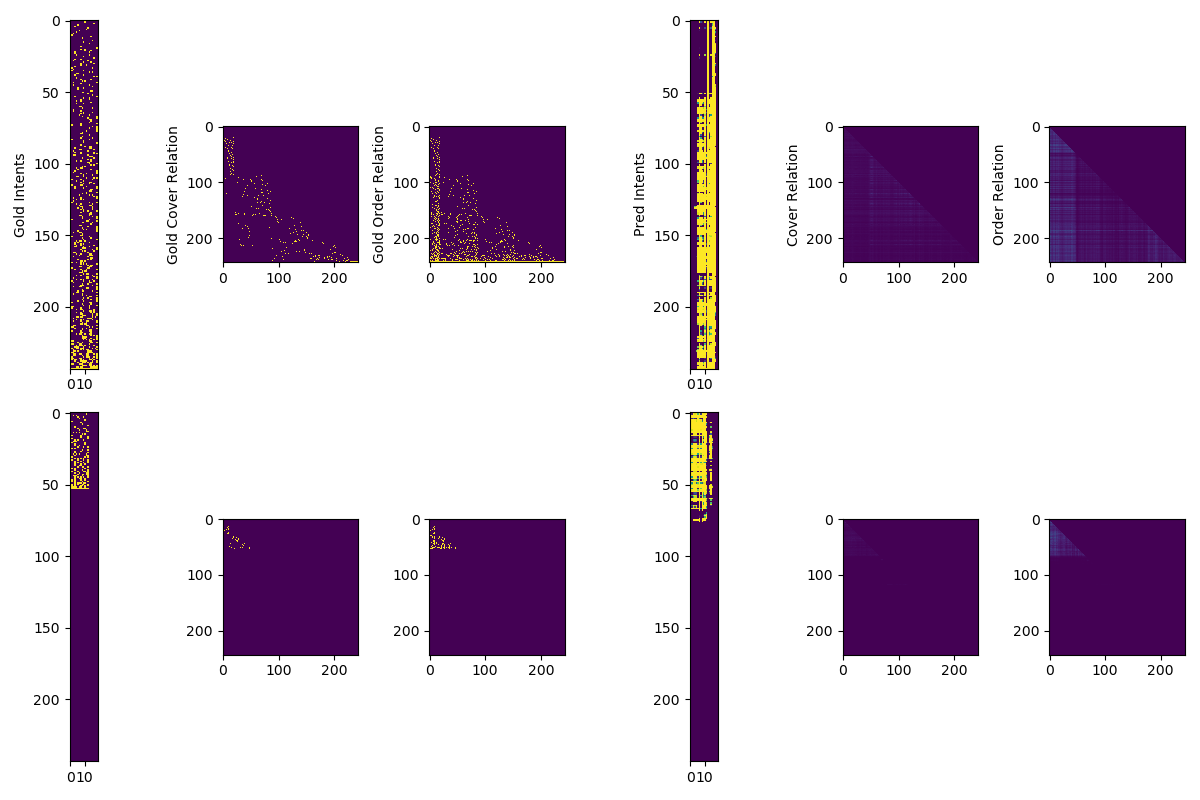
\includegraphics[keepaspectratio, width=.9\textwidth]{Figures/Ch3/concept_small.png}
    \caption{Batch of 2 samples (one per row) of the evaluation set and the predictions of our model. The first three columns correspond to the sample itself, and the last three to the model's prediction.}
    \label{fig:fcat-perf}
\end{figure}

\chapter{Conclusion and Discussion\label{ch:ccl}}
% Do not forget to position your work in the realm of cognitive science/NLP.
% Conclude with the successes you have gained at this internship, and possibly critiques. Specify what you may have missed in your university education, perhaps also what has particularly served you.

In this internship, we explored methods to reproduce FCA using NNs by focusing on the generation of concept lattices.
The task we tackled is not much documented. To bridge this gap in the literature, we conduct a very exploratory work.

Our initial approach relied on GraphRNN, and did not produce the intended results.
However, it allowed us to tackle multiple challenges.
First, we developed a data format to represent lattices in a way usable in deep learning.
To achieve this, we designed a concept ordering based on what we call levels, in replacement for the breadth-first search used in GraphRNN. %\todo{faire plus clair (comme si pas lu le rapport}
Then, handling GraphRNN led us to explore multiple methods to represent and manipulate adjacency matrices for $\leq$ and $\prec$.

Finally, we addressed the problem of the representation of FCs of any size.
%
To handle this challenging task, we developed BoA, an embedding architecture for FCs.
This embedding method is flexible and data agnostic, and is published in the workshop FCA4AI of the conference ECAI with the article~\cite{boa:2020:marquer}.
Most of the properties of BoA were designed towards intent generation.
For instance, to train BoA, we designed a similarity measure for attributes based on their co-appearance in the intents, the co-intent similarity. %\todo{faire plus soft}

%Motivated by the task of intent generation, 
We evolved our approach to make the most of the properties of the new BoA model by centering the architecture on intent generation.
%To profit from the properties of the new BoA model, we evolved our approach by centering it on intent prediction.
Along the way, we designed a simple and effective model to predict a reasonable upper bound of the number of concepts.
Our intent model uses a variety of attention mechanisms along with an LSTM to predict intent embeddings.
This design decision was led by preliminary tests on multiple common architectures.
It is interesting to note that we reproduce the inner process of GraphRNN with our self attention mechanism.
Indeed, we iteratively add intents and predict their relation with previous intents, similarly to how GraphRNN handles adjacency.

The performance of the intent model is heavily dependent on the quality of the BoA model.
As observed in~\cite{boa:2020:marquer}, the current BoA can be improved in several ways.
For instance, the co-intent similarity is not correctly predicted.
We expect that embeddings already containing this notion of intent would greatly improve the performance of the generative model.
%We have many tracks to improving BoA, that will be explored and published during the beginning of our Ph.D.
Due to time constraints, we were unable to finalize the approach.
However, we designed a first end-to-end intent model which provides baseline results for intent generation.
%We have many tracks to improving BoA, that will be explored and published during the beginning of our Ph.D.
%We have many tracks to improving BoA, but due to time constraints we preferred to finalize a first end-to-end intent model.
%That way, we would have a complete framework to test the impact of each improvement we will bring to the components.\todo{phrase courte: preparer d'autres features pour être soumis}
%\todo{due to time constraint, we were unable to finalize the approach..., (but continue to expore in the phd)}
%In the available time, we did not manage to implement the final ``refiner'' component of our intent model.
%However, we developed a complete intent model after exploring multiple variants, and provide baseline results for the intent generation task using NNs.
%
We have 3 main tracks to improve our current approach, that will be explored and published during the beginning of our Ph.D.
Firstly, improving BoA, the foundation of our approach, would positively impact the performance of the whole framework.
We are thinking of working on the variational aspect of the embedding model, in addition to rectifying the co-intent similarity prediction.
Secondly, adding the planned refiner and further training the full intent model would improve the performance.
Thirdly, we have plans to explore applications of BoA on other fields than FCA, \eg, pattern mining, sentiment analysis, and information retrieval.
%If those explorations are fruitfull, the intent generation architecture could be used 

%\todo{this last paragraph is ... meh}
Finally, we used a wide variety of models, from node and graph neural frameworks to complex generative models, passing by attention mechanism and embedding models based on FCA. Most of these models come from or are extensively developed in natural language processing (NLP). 
Firstly, recurrent architectures like LSTM are extensively used in language modeling.
Secondly, attention models first appeared for alignment automatic translation~\cite{attention:2015:bahdanau}. They were further developed in the transformer and reformer models~\cite{reformer:2020:kitaev,transformer:2017:vaswani}, both designed for translation too.
Thirdly, word2vec~\cite{word2vec:2013:mikolov} is one of the most famous word embedding architecture which was adapted in a wide variety of domains, including FCA with FCA2VEC~\cite{fca2vec:2019:durrschnabel} and node embedding with node2vec~\cite{node2vec:2016:grover}.
In a nutshell, a large portion of the work presented in this thesis relies on NNs used in NLP.
Additionally, FCA is well known to go from row data to knowledge and supports many semantic web tasks such as ontology building, \eg, extracting properties of pharmaceutical products from medical articles to build an ontology of pharmaceutical substances and their effects. The knowledge can then be fed back into NLP systems, \eg, a chatbot for medical monitoring.
%In conclusion, while FCA itself is a mathematical field of knowledge processing, it

%+ txt mining, info retrival
%+ sentiment analysis basée FCA

At the beginning of the internship, we lacked mathematical bases in lattice theory to make the most of the FCA process.
The fundamentals in FCA, ontologies and data mining that are taught in the NLP master of \textit{Université de Lorraine} greatly helped us to fill the blanks.
Furthermore, our accumulated expertise in a wide variety of models used in NLP helped us in manipulating the NN architectures we encountered.
It also helped us in developing a meaningful approach to FC embedding and intent generation.

%\appendix % Cue to tell LaTeX that the following "chapters" are Appendices
%\chapter{Modifications applied} % Main appendix title
\label{app:graphrnn-mods}

In this appendix we present some of the modifications we tested to improve the performance of the GraphRNN VAE.

\section{Sharing and Pre-Training the Node-Level Model}

\section{Stop Loss}
stop vector VS I/O vector
BCE on individual positions

\section{Pseudo-Transitive Closure Loss}
Pseudo-transitivity as a differential alternative to transitivity, instead of BCE
in practice, values are number of pathes between Top and this node

\section{Training the Decoder With or Without Gold Input}
provide expected sequence as a tensor, in a more standard seq2seq setting

%\input{Appendices/canonical_base}


\printbibliography[heading=bibintoc]




% The report should be send to the head of the second year and the University supervisor at least 8 days before the defense (strict) (digital copy and hard copy if it asked by the university supervisor). You must provide a hard copy for the head of the second year before the defense.
% M2 Defence: September 2-3th (report due on August 24th)
% M2 final jury: September 4th
%max 50p
